The systematics considered in the $HH$ analysis
is outlined in this section. For the same reason 
mentioned in section~\ref{sec:FTAG_systematics}, 
the systematic uncertainties can be broadly catergorised
into experimental and modelling systematic uncertainties. 
The former arise from experimental sources related to the detector 
response and the physics object reconstruction and identification,
while the modelling systematic uncertainties account for 
theoretical uncertainties related to the limited 
knowledge of the MC simulated processes 
and uncertainties on data-driven backgrounds. 
The experimental and modelling uncertainties are derived for 
all backgrounds and signals, manifesting the overall yields
or the shape of the final discriminant, or both together.
All uncertainties considered are propagated through the analysis,
and are included in the statistical analysis fit
discussed in section~\ref{} TODO: ref fit section.


\subsection{Experimental uncertainties}
\label{sec:systematics_experimental}

Uncertainty of measuring the luminosity 
arises from calirating it with the van der Meer method~\cite{DAPR-2013-01}.
The uncertainty on the full Run 2 data is $\pm$1.7\%, obtained using the
LUCID (LUminosity measurement using a Cherenkov Integrating Detector)
detector~\cite{ATLAS-Lumi2}.

A reweighting is applied on the MC simlulations to match 
the pile-up condition in each data-taking period during Run 2~\cite{STDM-2015-05}. 
The uncertainty associated with the reweighting
is estimated by varing the reweighting factors used in the MC simulation. 

The uncertainties in single lepton triggers ($e$ or $mu$), 
uncertainties due to leptons reconstruction, identification and
isolation are estimated by varying the selection used in the
tag-and-probe method. 
In the tag-and-probe approach, stringent selection criterias are applied on one lepton,
and the other lepton is used for the efficiency measurement. 
For electrons, $Z\rightarrow e^+e^-$ events 
are used~\cite{EGAM-2018-01} while for muons, 
both $Z\rightarrow \mu^+\mu^-$  and $J/\psi\rightarrow \mu^+\mu^-$ events
are used~\cite{CERN-EP-2020-199}. 


The uncertainty on electron energy resolution is estimated by smearing the
electron energies in MC simulations, while 
the momentum scale and energy resolution variations are derived in 
$Z\rightarrow \mu^+\mu^-$  and $J/\psi\rightarrow \mu^+\mu^-$ events. 

Similarly for the \tauhad\ lepton, the tag-and-probe method is used
to measure the reconstruction and identification efficiency scale factors,
using $Z\rightarrow \tau^+\tau^-$ events~\cite{ATLAS-CONF-2017-029}.  
Uncertainties are estimated in the efficiencies of the electron veto for
\tauhad, using $Z\rightarrow e^+e^-$ events. 


The systematic uncertainties associated to the jet energy scale
calibration~\cite{JETM-2018-05}, 
as described in section~\ref{sec:jet}, are grouped into
a reduced-size set of nuisance parameters.
The reduced set is referred to as `CategoryReduction', 
and is recommended set of uncertainties for analyses
aiming to perform combinations with other searches. 
Similarly, the jet energy resolution uncertainties~\cite{JETM-2018-05}
are grouped in to the `FullJER' scheme for this reason.
The jet energy resolution uncertainties therefore are 
comprised of 30 nuisance parameters 
and 13 nuisance parameters for the jer energy resolution uncertainties. 

The uncertainty associated with the JVT algorithm (see section~\ref{sec:jet}) 
is estimated by varying the reqirements on the algorithm output discriminant. 


As described in section~\ref{sec:FTAG}, scale factors are measured 
to correct the \btagging\ efficiency in MC simulations to match the one in data. 
Uncertainties in the \btagging\ efficiency are considered
as a function of \pt\ for b-jets and c-jets using \ttbar\ events~
\cite{FTAG-2018-01,FTAG-paper}, 
and as a function of pT and $\eta$ for
light-flavour jets using di-jet events~\cite{ATLAS-CONF-2018-006}.
The `medium reduction' scheme is used, which is
the preferred reduction scheme used for analyses aiming for combination. 
It contains 13 nuisance parameters, 3 for \bjets, 4 for \cjets, 
4 for light-jets and 2 for extrapolations.


The energy scale and resolution uncertainties mentioned above, 
in addition to an uncertainty in the tracks matched to the primary vertex 
but not associated to other reconstructed objects in the event, are
propagated to the \met calculation~\cite{PERF-2016-07}.




\begin{table}
    \centering
    \tiny
    \begin{tabular}{|c|c|}
    \hline
    NP Name & Description\\
    \hline
    \multicolumn{2}{|c|}{ Event } \\
    \hline
    ATLAS\textunderscore LUMI\textunderscore Run2 & Uncertainty on the total integrated luminosity (1.7\%)\\
    ATLAS\textunderscore PU\textunderscore PRW\textunderscore DATASF & Pile-up reweighting\\
    \hline
    \multicolumn{2}{|c|}{ electrons }\\
    \hline
    EL\textunderscore EFF\textunderscore TRIG\textunderscore TOTAL\textunderscore 1NPCOR\textunderscore PLUS\textunderscore UNCOR & electron-trigger \\
    EL\textunderscore EFF\textunderscore RECO\textunderscore TOTAL\textunderscore 1NPCOR\textunderscore PLUS\textunderscore UNCOR & electron-reconstruction\\
    EL\textunderscore EFF\textunderscore ID\textunderscore TOTAL\textunderscore 1NPCOR\textunderscore PLUS\textunderscore UNCOR & electron-identification\\
    EL\textunderscore EFF\textunderscore ISO\textunderscore TOTAL\textunderscore 1NPCOR\textunderscore PLUS\textunderscore UNCOR & electron-isolation\\
    \hline
    \multicolumn{2}{|c|}{ muons }\\
    \hline
    MUON\textunderscore EFF\textunderscore TrigStatUncertainty & mun-trigger\\
    MUON\textunderscore EFF\textunderscore TrigSystUncertainty & \\
    MUON\textunderscore EFF\textunderscore RECO\textunderscore STAT & muon-reconstruction\\
    MUON\textunderscore EFF\textunderscore RECO\textunderscore SYS & \\
    MUON\textunderscore EFF\textunderscore RECO\textunderscore STAT\textunderscore LOWPT & \\
    MUON\textunderscore EFF\textunderscore RECO\textunderscore SYS\textunderscore LOWPT & \\
    MUON\textunderscore EFF\textunderscore ISO\textunderscore STAT & muon-isolation\\
    MUON\textunderscore EFF\textunderscore ISO\textunderscore SYS & \\
    MUON\textunderscore EFF\textunderscore TTVA\textunderscore STAT & muon-TTVA\\
    MUON\textunderscore EFF\textunderscore TTVA\textunderscore SYS & \\
    MUON\textunderscore ID & muon-momentum calibration \\
    MUON\textunderscore MS & \\
    MUON\textunderscore SCALE & \\
    MUON\textunderscore SAGITTA\textunderscore RHO & \\
    MUON\textunderscore SAGITTA\textunderscore RESBIAS & \\
    \hline
    \multicolumn{2}{|c|}{ $\tau$-leptons }\\
    \hline
    TAUS\textunderscore TRUEHADTAU\textunderscore EFF\textunderscore TRIGGER\textunderscore STATDATA161718 & $\tau$-trigger\\
    TAUS\textunderscore TRUEHADTAU\textunderscore EFF\textunderscore TRIGGER\textunderscore STATDATA1718 & \\
    TAUS\textunderscore TRUEHADTAU\textunderscore EFF\textunderscore TRIGGER\textunderscore STATDATA2016 & \\
    TAUS\textunderscore TRUEHADTAU\textunderscore EFF\textunderscore TRIGGER\textunderscore STATDATA2018 & \\
    TAUS\textunderscore TRUEHADTAU\textunderscore EFF\textunderscore TRIGGER\textunderscore STATDATA2018AFTTS1 & \\
    TAUS\textunderscore TRUEHADTAU\textunderscore EFF\textunderscore TRIGGER\textunderscore STATMC161718 &\\
    TAUS\textunderscore TRUEHADTAU\textunderscore EFF\textunderscore TRIGGER\textunderscore STATMC1718 & \\
    TAUS\textunderscore TRUEHADTAU\textunderscore EFF\textunderscore TRIGGER\textunderscore STATMC2016 & \\
    TAUS\textunderscore TRUEHADTAU\textunderscore EFF\textunderscore TRIGGER\textunderscore STATMC2018 & \\
    TAUS\textunderscore TRUEHADTAU\textunderscore EFF\textunderscore TRIGGER\textunderscore STATMC2018AFTTS1 & \\
    TAUS\textunderscore TRUEHADTAU\textunderscore EFF\textunderscore TRIGGER\textunderscore SYST161718 & \\
    TAUS\textunderscore TRUEHADTAU\textunderscore EFF\textunderscore TRIGGER\textunderscore SYST1718 & \\
    TAUS\textunderscore TRUEHADTAU\textunderscore EFF\textunderscore TRIGGER\textunderscore SYST2016 & \\
    TAUS\textunderscore TRUEHADTAU\textunderscore EFF\textunderscore TRIGGER\textunderscore SYST2018 & \\
    TAUS\textunderscore TRUEHADTAU\textunderscore EFF\textunderscore TRIGGER\textunderscore SYST2018AFTTS1& \\
    TAUS\textunderscore TRUEHADTAU\textunderscore EFF\textunderscore TRIGGER\textunderscore SYSTMU161718 & \\
    TAUS\textunderscore TRUEHADTAU\textunderscore EFF\textunderscore TRIGGER\textunderscore SYSTMU1718 & \\
    TAUS\textunderscore TRUEHADTAU\textunderscore EFF\textunderscore TRIGGER\textunderscore SYSTMU2016 & \\
    TAUS\textunderscore TRUEHADTAU\textunderscore EFF\textunderscore TRIGGER\textunderscore SYSTMU2018 & \\
    TAUS\textunderscore TRUEHADTAU\textunderscore EFF\textunderscore TRIGGER\textunderscore SYSTMU2018AFTTS1& \\
    TAUS\textunderscore TRUEHADTAU\textunderscore EFF\textunderscore RECO\textunderscore HIGHPT & $\tau$-reconstruction\\
    TAUS\textunderscore TRUEHADTAU\textunderscore EFF\textunderscore RECO\textunderscore TOTAL & \\
    TAUS\textunderscore TRUEHADTAU\textunderscore EFF\textunderscore RNNID\textunderscore 1PRONGSTATSYSTPT2025 & $\tau$-odentification\\
    TAUS\textunderscore TRUEHADTAU\textunderscore EFF\textunderscore RNNID\textunderscore 1PRONGSTATSYSTPT2530 & \\
    TAUS\textunderscore TRUEHADTAU\textunderscore  EFF\textunderscore RNNID\textunderscore 1PRONGSTATSYSTPT3040 & \\
    TAUS\textunderscore TRUEHADTAU\textunderscore EFF\textunderscore RNNID\textunderscore 1PRONGSTATSYSTPTGE40 & \\
    TAUS\textunderscore TRUEHADTAU\textunderscore EFF\textunderscore RNNID\textunderscore 3PRONGSTATSYSTPT2025 & \\
    TAUS\textunderscore TRUEHADTAU\textunderscore EFF\textunderscore RNNID\textunderscore 3PRONGSTATSYSTPT2530 & \\
    TAUS\textunderscore TRUEHADTAU\textunderscore EFF\textunderscore RNNID\textunderscore 3PRONGSTATSYSTPT3040 & \\
    TAUS\textunderscore TRUEHADTAU\textunderscore EFF\textunderscore RNNID\textunderscore 3PRONGSTATSYSTPTGE40 & \\
    TAUS\textunderscore TRUEHADTAU\textunderscore EFF\textunderscore RNNID\textunderscore HIGHPT &\\
    TAUS\textunderscore TRUEHADTAU\textunderscore EFF\textunderscore RNNID\textunderscore SYST &\\
    TAUS\textunderscore TRUEHADTAU\textunderscore SME\textunderscore TES\textunderscore INSITUEXP & $\tau$-energy scale\\
    TAUS\textunderscore TRUEHADTAU\textunderscore SME\textunderscore TES\textunderscore INSITUFIT &\\
    TAUS\textunderscore TRUEHADTAU\textunderscore SME\textunderscore TES\textunderscore MODEL\textunderscore CLOSURE &\\
    TAUS\textunderscore TRUEHADTAU\textunderscore SME\textunderscore TES\textunderscore PHYSICSLIST &\\
    TAUS\textunderscore TRUEELECTRON\textunderscore EFF\textunderscore ELEBDT\textunderscore STAT & $\tau$-electron veto\\
    TAUS\textunderscore TRUEELECTRON\textunderscore EFF\textunderscore ELEBDT\textunderscore SYST &\\
    TAUS\textunderscore TRUEHADTAU\textunderscore EFF\textunderscore ELEOLR\textunderscore TOTAL &\\
    \hline
    \multicolumn{2}{|c|}{ egamma }\\
    \hline
    EG\textunderscore RESOLUTION\textunderscore ALL & egamma resolution\\
    EG\textunderscore SCALE\textunderscore ALL & egamma scale\\
    EG\textunderscore SCALE\textunderscore AF2 & \\
    \hline
    \multicolumn{2}{|c|}{ \MET }\\
    \hline
    MET\textunderscore SoftTrk\textunderscore ResoPar a & \\
    MET\textunderscore SoftTrk\textunderscore ResoPerp & \\
    MET\textunderscore SoftTrk\textunderscore ScaleDown & \\
    MET\textunderscore SoftTrk\textunderscore ScaleUp & \\
    \hline
    \end{tabular}
    \caption{List of experimental systematic uncertainties. Table reproduced from analysis internal notes. 
    }
    \label{tab:systematics_experimental_list}
    \end{table}
    
    \begin{table}
    \centering
    \tiny
    \begin{tabular}{|c|c|}
    \hline
    NP Name & Description\\
    \hline
    \multicolumn{2}{|c|}{ Jets }\\
    \hline
    JET\textunderscore EtaIntercalibration\textunderscore Modelling & Jet energy scale (CategoryReduction)\\
    JET\textunderscore EtaIntercalibration\textunderscore TotalStat & \\
    JET\textunderscore EtaIntercalibration\textunderscore NonClosure\textunderscore highE & \\
    JET\textunderscore EtaIntercalibration\textunderscore NonClosure\textunderscore negEta & \\
    JET\textunderscore EtaIntercalibration\textunderscore NonClosure\textunderscore posEta & \\
    JET\textunderscore Pileup\textunderscore OffsetMu & \\                
    JET\textunderscore Pileup\textunderscore OffsetNPV & \\
    JET\textunderscore Pileup\textunderscore PtTerm & \\            
    JET\textunderscore Pileup\textunderscore RhoTopology & \\             
    JET\textunderscore Flavor\textunderscore Composition & \\
    JET\textunderscore Flavor\textunderscore Response & \\            
    JET\textunderscore PunchThrough\textunderscore MC16 & \\             
    JET\textunderscore PunchThrough\textunderscore AFII & \\
    JET\textunderscore EffectiveNP\textunderscore Detector1 & \\
    JET\textunderscore EffectiveNP\textunderscore Detector2 & \\
    JET\textunderscore EffectiveNP\textunderscore Mixed1 & \\
    JET\textunderscore EffectiveNP\textunderscore Mixed2 & \\
    JET\textunderscore EffectiveNP\textunderscore Mixed3 & \\
    JET\textunderscore EffectiveNP\textunderscore Modelling1 & \\
    JET\textunderscore EffectiveNP\textunderscore Modelling2 & \\
    JET\textunderscore EffectiveNP\textunderscore Modelling3 & \\
    JET\textunderscore EffectiveNP\textunderscore Modelling4 & \\
    JET\textunderscore EffectiveNP\textunderscore Statistical1 & \\
    JET\textunderscore EffectiveNP\textunderscore Statistical2 & \\
    JET\textunderscore EffectiveNP\textunderscore Statistical3 & \\
    JET\textunderscore EffectiveNP\textunderscore Statistical4 & \\
    JET\textunderscore EffectiveNP\textunderscore Statistical5 & \\
    JET\textunderscore EffectiveNP\textunderscore Statistical6 & \\
    JET\textunderscore SingleParticle\textunderscore HighPt & \\          
    JET\textunderscore RelativeNonClosure\textunderscore AFII & \\
    JET\textunderscore BJES\textunderscore Response & \\             
    JET\textunderscore EtaIntercalibration\textunderscore NonClosure\textunderscore 2018data & \\
    JET\textunderscore JER\textunderscore DataVsMC\textunderscore MC16 & Jet energy resolution (FullJer) \\
    JET\textunderscore JER\textunderscore DataVsMC\textunderscore AFI & \\I 
    JET\textunderscore JER\textunderscore EffectiveNP\textunderscore 1 & \\
    JET\textunderscore JER\textunderscore EffectiveNP\textunderscore 2 & \\   
    JET\textunderscore JER\textunderscore EffectiveNP\textunderscore 3 & \\
    JET\textunderscore JER\textunderscore EffectiveNP\textunderscore 4 & \\   
    JET\textunderscore JER\textunderscore EffectiveNP\textunderscore 5 & \\
    JET\textunderscore JER\textunderscore EffectiveNP\textunderscore 6 & \\   
    JET\textunderscore JER\textunderscore EffectiveNP\textunderscore 7 & \\
    JET\textunderscore JER\textunderscore EffectiveNP\textunderscore 8 & \\   
    JET\textunderscore JER\textunderscore EffectiveNP\textunderscore 9 & \\
    JET\textunderscore JER\textunderscore EffectiveNP\textunderscore 10 & \\  
    JET\textunderscore JER\textunderscore EffectiveNP\textunderscore 11 & \\
    JET\textunderscore JER\textunderscore EffectiveNP\textunderscore 12restTerm & \\
    JET\textunderscore JVT\textunderscore EFF & Jet vertex tagging \\
    JET\textunderscore FJVT\textunderscore EFF & Forward jet vertex tagging \\
    \hline
    \multicolumn{2}{|c|}{ $b$-tagging }\\
    \hline
    FT\textunderscore EFF\textunderscore Eigen\textunderscore B\textunderscore 0& \\
    FT\textunderscore EFF\textunderscore Eigen\textunderscore B\textunderscore 1 & \\
    FT\textunderscore EFF\textunderscore Eigen\textunderscore B\textunderscore 2 & \\
    FT\textunderscore EFF\textunderscore Eigen\textunderscore C\textunderscore 0 & \\
    FT\textunderscore EFF\textunderscore Eigen\textunderscore C\textunderscore 1 & \\
    FT\textunderscore EFF\textunderscore Eigen\textunderscore C\textunderscore 2 & \\
    FT\textunderscore EFF\textunderscore Eigen\textunderscore C\textunderscore 3 & \\
    FT\textunderscore EFF\textunderscore Eigen\textunderscore Light\textunderscore 0 & \\
    FT\textunderscore EFF\textunderscore Eigen\textunderscore Light\textunderscore 1 & \\
    FT\textunderscore EFF\textunderscore Eigen\textunderscore Light\textunderscore 2 & \\
    FT\textunderscore EFF\textunderscore Eigen\textunderscore Light\textunderscore 3 & \\
    FT\textunderscore EFF\textunderscore extrapolation & \\
    FT\textunderscore EFF\textunderscore extrapolation\textunderscore from\textunderscore charm & \\
    \hline
    \end{tabular}
    \caption{List of experimental systematic uncertainties. Table reproduced from analysis internal notes. 
    }
    \label{tab:systematics_experimental_list_2}
    \end{table}




\subsection{Background modelling uncertainties for MC-based processes}
\label{sec:systematics_backgroundmodelling}

The background modelling uncertainties on
 MC-based processed include theoretical cross section and acceptance uncertainties. 

The list of all uncertainties applied to all MC-based backgrounds is reported in Table~\ref{sec:systs:tab:systematics_normalisations_list_Major} and Table~\ref{sec:systs:tab:systematics_normalisations_list_Minor}. 

Cross section uncertainties only affect normalisations and are applied to all backgrounds with normalisations estimated from MC (following the Physics Modelling Group recommendations).

Acceptance uncertainties can affect both normalisations and shapes. Their contribution is usually divided into a normalisation acceptance uncertainty, that affects the number of events predicted in the signal region, and a shape uncertainty affecting the shape of the final discriminant distribution. 

The acceptance uncertainties applied on minor backgrounds (Z+lf, W+jets, and Diboson) are taken from the SM Vhbb analysis~\cite{ATLAS-CONF-2020-006} as described in Section~\ref{subsec:uncertainties_minor_bkgs}. Acceptance uncertainties for $t\bar{t}$, Z+HF, single-top (Wt channel), ttH and ZH are estimated in the phase-space of signal and control regions of this analysis from comparisons between nominal and alternative MC simulated samples as described in the following dedicated Sections. 

The normalisation acceptance uncertainties are derived comparing the acceptance obtained for each alternative sample 'i' to the nominal acceptance, which corresponds to the comparison of the number of the expected events for each variation 'i' to the nominal expected events in the signal region when the samples are all normalised to the same cross section:

\begin{equation}
\sigma_{Acc}^{i}= \frac{Acc_{variation}^{i} - Acc_{nominal}}{Acc_{nominal}} = \frac{N_{variation}^{i}-N_{nominal}}{N_{nominal}}\,.
\label{eq:acceptance_unc}
\end{equation}

When several regions are included in the final fit and the normalisation of the process is derived from data (constrained mainly from one of the regions), a relative normalisation acceptance uncertainty can be estimated from the comparison of the relative amount of events predicted by the alternative model in one region “A” with respect to another region “B” and the same fraction in the nominal model:%, which can be calculated from the ratio of the acceptance uncertainties of the two regions:

%\begin{equation}
%\sigma_{Acc_{A}/Acc_{B}}= \frac{\frac{Acc_{variation, A}}{Acc_{variation, B}} - \frac{Acc_{nominal, A}}{Acc_{nominal, B}}} {\frac{Acc_{nominal, A}}{Acc_{nominal, B}}} = \frac{Acc_{variation, A}}{Acc_{nominal, A}} /  \frac{Acc_{variation, B}}{Acc_{nominal, B}} -1  = \frac{\sigma_{Acc, A}}{\sigma_{Acc, B}} -1 \,.
%\label{eq:relative_acceptance_unc}
%\end{equation}

\begin{equation}
\sigma_{Acc_{A}/Acc_{B}}= \frac{\frac{Acc_{variation, A}}{Acc_{variation, B}} - \frac{Acc_{nominal, A}}{Acc_{nominal, B}}} {\frac{Acc_{nominal, A}}{Acc_{nominal, B}}} = \frac{\frac{N_{variation, A}}{N_{variation, B}} - \frac{N_{nominal, A}}{N_{nominal, B}}} {\frac{N_{nominal, A}}{N_{nominal, B}}}\;.
\label{eq:relative_acceptance_unc}
\end{equation}

Acceptance uncertainties on the normalisation of the backgrounds are applied in all regions and treated as correlated across regions except for the $t\bar{t}$ and Z+HF backgrounds whose normalisations are left unconstrained (floated) in the global likelihood fit. For these two processes relative acceptance uncertainties between regions with a common underlying normalisation are applied. 

Acceptance effects on the shapes are treated separately as they do not change the amount of expected events (this is a technical choice done to disentangle the two effects and have the possibility to identify the effects that have a larger impact on the result). The shape uncertainties are derived comparing the distributions of several kinematical variables of the alternative samples to the ones of the nominal sample. The comparison is done by taking the normalised distributions (to exclude the normalisation effects that are considered separately) and calculating the ratio of the alternative and nominal number of events bin per bin. 

Details are described in the following dedicated sections where also shape uncertainties are described where applied.


\begin{table}
\centering
\tiny
\begin{tabular}{|c|c|c|c|c|c|}
\hline
Process & Name & HadHad SR & LepHad SLT SR & LepHad LTT SR & Comment\\
\hline
ttbar & THEO\textunderscore ACC \textunderscore TTBAR\textunderscore ME & N: +0.037, -0.037, S & N: +0.0026, -0.0026, S & N: -0.009, +0.009 & Matrix element acceptance \\
ttbar & THEO\textunderscore ACC \textunderscore TTBAR\textunderscore PS & N: -0.022, +0.022, S & N: -0.072, +0.072, S & N: -0.088, +0.088 & Parton shower acceptance\\
ttbar & THEO\textunderscore ACC \textunderscore TTBAR\textunderscore ISR & N: -0.0002, -0.003, S & N: +0.0005, -0.0081 & N:-0.0052, +0.013  & ISR acceptance \\
ttbar & THEO\textunderscore ACC \textunderscore TTBAR\textunderscore FSR & N: +0.019, -0.045, S & N: +0.014, -0.0097 & N: +0.0096, -0.032 & FSR acceptance \\
ttbar & THEO\textunderscore ACC \textunderscore TTBAR\textunderscore PDFalphas & N: -0.0011, +0.0011 & N: -0.006, +0.006 & N: -0.0011, +0.0011 & PDF+$\alpha_s$ acceptance \\
Z+hf & THEO\textunderscore ACC\textunderscore Zhf\textunderscore GENERATOR & N: -0.07, +0.07, S & N: +0.021, -0.021 & N: +0.10, -0.10 & Matrix element acceptance\\ 
Z+hf & THEO\textunderscore ACC\textunderscore Zhf\textunderscore SCALE & N: -0.096, +0.12, S & N: -0.029, +0.053, S & N: -0.054, +0.085, S & Scale acceptance\\
Z+hf & THEO\textunderscore ACC\textunderscore Zhf\textunderscore CKKW & N: +0.053, -0.053 & N: +0.07, -0.07 & N: +0.071, -0.071 & CKKW acceptance\\
Z+hf & THEO\textunderscore ACC\textunderscore Zhf\textunderscore QSF & N: +0.06, -0.06 & N: -0.016, +0.016 & N: -0.016 , +0.016 & QSF acceptance\\
Z+hf & THEO\textunderscore ACC\textunderscore Zhf\textunderscore PDFalphas & N: -0.0077, +0.0077 & N: -0.0026, +0.0026 & N: -0.0033 , +0.0033 & PDF+$\alpha_s$ acceptance\\
Z+hf & THEO\textunderscore ACC\textunderscore Zhf\textunderscore PDFChoice & N: -0.0098, +0.0098 & N: -0.0097, +0.0097 & N: -0.011, +0.011 & PDF choice acceptance\\
stopWt & THEO\textunderscore XS\textunderscore Stop & N: -0.054,+0.054 & N: -0.054, +0.054 & N: -0.054, +0.054 & cross section\\
stopWt & THEO\textunderscore ACC\textunderscore StopWt\textunderscore ME & N: +0.049, -0.049 & N: - 0.022, +0.022 & N: -0.15, 0.15 & Matrix element acceptance\\
stopWt & THEO\textunderscore ACC\textunderscore StopWt\textunderscore PS & N: -0.16, +0.16 & N: +0.077, -0.077 & N: -0.093, +0.093& Parton shower acceptance\\
stopWt & THEO\textunderscore ACC\textunderscore StopWt\textunderscore ISR & N:  -0.049, +0.066 & N: -0.047, +0.064 & N: -0.045, +0.062& ISR acceptance\\
stopWt & THEO\textunderscore ACC\textunderscore StopWt\textunderscore FSR & N: -0.094, +0.087 & N: -0.054, +0.043 & N: -0.069, +0.035 & FSR acceptance\\
stopWt & THEO\textunderscore ACC\textunderscore StopWt\textunderscore PDF & N: -0.032, +0.032 & N: -0.032, +0.032 & N: -0.032, +0.032 & PDF acceptance\\
stopWt & THEO\textunderscore ACC\textunderscore StopWt\textunderscore TopInterference & N: +0.27, -0.27 , S & N: +0.078, -0.078, S & N: +0.11, +0.11, S & top interference acceptance\\
ttH & THEO\textunderscore XS\textunderscore SCALE\textunderscore ttH & N: -0.092, +0.058 & N: -0.092, +0.058 & N: -0.092, +0.058 & Scale cross section\\
ttH & THEO\textunderscore XS\textunderscore PDFalphas\textunderscore ttH & N: -0.036, +0.036 & N: -0.036, +0.036 & N: -0.036, +0.036 & PDF+$\alpha_s$ cross section\\
ttH & THEO\textunderscore ACC\textunderscore GEN\textunderscore ttH & N: -0.033, +0.033 & - & N: -0.019, +0.019 & Matrix element acceptance\\
ttH & THEO\textunderscore ACC\textunderscore PS\textunderscore ttH & N: -0.011, +0.011  & N: -0.013, +0.013 & N: -0.067, +0.067 & Parton shower acceptance\\
ttH & THEO\textunderscore ACC\textunderscore SCALE\textunderscore ttH & N:-0.01, +0.01 & - & - & Scale acceptance\\
ttH & THEO\textunderscore ACC\textunderscore ISR\textunderscore ttH & - & - & N: -0.01, +0.01 & ISR acceptance\\
ttH & THEO\textunderscore ACC\textunderscore FSR\textunderscore ttH & N: -0.06, +0.037,  &  N: -0.051, +0.032, & N: -0.15 , +0.055 & FSR acceptance\\
ggFHtautau & THEO\textunderscore XS\textunderscore SCALE\textunderscore ggFH & N: -0.039, +0.039 & N: -0.039, +0.039 & N: -0.039, +0.039 & Scale cross section\\
ggFHtautau & THEO\textunderscore XS\textunderscore PDFalphas\textunderscore ggFH & N: -0.032, +0.032 & N: -0.032, +0.032 & N: -0.032, +0.032 & PDF+$\alpha_s$ section\\
ggF, ZH, WH, VBFH with Htautau & THEO\textunderscore BR\textunderscore Htautau & N: -0.02, +0.02 & N: -0.02, +0.02 & N: -0.02, +0.02 & Htautau BR\\
ggFHtautau & THEO\textunderscore ACC\textunderscore HF\textunderscore ggFH & N: -1.0, +1.0 & N: -1.0, +1.0 & N: -1.0, +1.0 & Higgs + HF mod unc\\
qqZHbb, qqZHtautau & THEO\textunderscore XS\textunderscore SCALE\textunderscore qqZH & N: -0.006,+0.005, & N: -0.006,+0.005, & -0.006, +0.005 & Scale cross section\\
qqZHbb, qqZHtautau & THEO\textunderscore XS\textunderscore PDFalphas\textunderscore qqZH & N: -0.019, +0.019 & N: -0.019, +0.019 &N:  -0.019, +0.019 & PDF+$\alpha_s$ cross section\\
ggZHbb, ggZHtautau & THEO\textunderscore XS\textunderscore SCALE\textunderscore ggZH & N: -0.19, +0.25, & N: -0.19 +0.25, & N: -0.19 , +0.25 & Scale cross section\\
ggZHbb, ggZHtautau & THEO\textunderscore XS\textunderscore PDFalphas\textunderscore qqZH & N: -0.024, +0.024 & N: -0.024, +0.024 & N: -0.024, +0.024 & PDF+$\alpha_s$ cross section\\
ZHbb, WHbb & THEO\textunderscore BR\textunderscore Hbb & N: -0.013, +0.013 & N: -0.013, +0.013 & N: -0.013, +0.013 & Hbb BR\\
ZHbb & THEO\textunderscore ACC\textunderscore PS\textunderscore ZHbb & N: -0.12, +0.12 &  N: -0.11, +0.11 & N: -0.037, +0.037 & Parton shower acceptance\\
ZHbb & THEO\textunderscore ACC\textunderscore SCALE\textunderscore ZHbb & N: -0.018, +0.018 & N: -0.030, +0.030 & N: -0.025, +0.025 & Scale acceptance\\
ZHtautau & THEO\textunderscore ACC\textunderscore PS\textunderscore ZHtautau & N: -0.056, +0.056 & N: -0.055, +0.055 & N: -0.15, +0.15  & Parton shower acceptance\\
ZHtautau & THEO\textunderscore ACC\textunderscore PDFalphas\textunderscore ZHtautau &  N: -0.01, +0.01 & - &  N: -0.012, +0.012 & PDF+$\alpha_s$ acceptance\\
ZHtautau & THEO\textunderscore ACC\textunderscore SCALE\textunderscore ZHtautau & N: -0.026, +0.026 & N: -0.022, +0.022 & N: -0.028, +0.028 & Scale acceptance\\
WHbb, WHtautau & THEO\textunderscore XS\textunderscore SCALE\textunderscore WH & N: -0.007, +0.005 & N: -0.007, +0.005 & N: -0.007  , +0.005 & Scale cross section\\
WHbb, WHtautau & THEO\textunderscore XS\textunderscore PDFalphas\textunderscore WH & N: -0.019, +0.019  & N: -0.019, +0.019 & N: -0.019, +0.019 & PDF+$\alpha_s$ cross section\\ 
WHtautau & THEO\textunderscore ACC\textunderscore HF\textunderscore WH &N: -1.0, +1.0 & N: -1.0, +1.0 & N: -1.0, +1.0 & Higgs + HF mod unc\\
VBFHtautau & THEO\textunderscore XS\textunderscore SCALE\textunderscore VBFH & N: -0.003, +0.004 & N: -0.003, +0.004 & -0.003, +0.004 & Scale cross section \\
VBFHtautau & THEO\textunderscore XS\textunderscore PDFalphas\textunderscore VBFH  & N: -0.021, +0.021 & N: -0.021, +0.021 & N: -0.021, +0.021 & PDF+$\alpha_s$ cross section \\
VBFHtautau & THEO\textunderscore ACC\textunderscore HF\textunderscore VBFH & N: -1.0, +1.0 & N: -1.0, +1.0 & N: -1.0, +1.0 & Higgs + HF mod unc\\
\hline
\end{tabular}
\caption{List of MC background uncertainties for major backgrounds. The table shows the process, the name of the uncertainty, the relative size of the normalisation uncertainty (N) and whether the uncertainty includes also a shape variation (S) in the different SRs.}
\label{sec:systs:tab:systematics_normalisations_list_Major}
\end{table}

\begin{table}
\centering
\tiny
\begin{tabular}{|c|c|c|c|}
\hline
Process & Name & Size & Comment\\
\hline
V+jets & THEO\textunderscore XS\textunderscore V & -0.05, +0.05 & cross section\\
Z+lf & THEO\textunderscore ACC\textunderscore Zlf & -0.23, +0.23 & Acceptance from VHbb\\
W+jets & THEO\textunderscore ACC\textunderscore W & -0.37, +0.37 & Acceptance from VHbb in LepHad SRs\\
W+jets & THEO\textunderscore ACC\textunderscore W & -0.50, +0.50 &  Acceptance inflated from VHbb analysis for tau fakes in HadHad SR\\
WW, WZ, ZZ & THEO\textunderscore XS\textunderscore Diboson & -0.06, +0.06 & cross section\\ 
WW & THEO\textunderscore ACC\textunderscore Diboson & -0.25, +0.25 & Acceptance from VHbb\\
WZ &  THEO\textunderscore ACC\textunderscore Diboson & -0.26, +0.26 & Acceptance from VHbb\\
ZZ & THEO\textunderscore ACC\textunderscore Diboson & -0.20, +0.20 & Acceptance from VHbb\\
\hline
\end{tabular}
\caption{List of MC background uncertainties for minor backgrounds. The table shows the process, the name of the uncertainty, the relative size of the normalisation uncertainty (N).}
\label{sec:systs:tab:systematics_normalisations_list_Minor}
\end{table}



%\begin{table}
%\centering
%\tiny
%\begin{tabular}{|c|c|c|c|}
%\hline
%Process & Size of Uncertainty & Name & Comment\\
%\hline
%ttbar & 0.06 & THEO\textunderscore XS\textunderscore ttbar & cross section\\
%ttbar & +0.037, -0.037 & TTBAR\textunderscore ACC\textunderscore ME\textunderscore MVA & ME in HadHad SR\\
%ttbar & -0.022, +0.022 & TTBAR\textunderscore ACC\textunderscore PS\textunderscore MVA & PS in HadHad SR\\
%ttbar & -0.0002, -0.003 & TTBAR\textunderscore ACC\textunderscore ISR\textunderscore MVA & ISR in HadHad SR\\
%ttbar & +0.019, -0.045 & TTBAR\textunderscore ACC\textunderscore FSR & FSR in HadHad SR\\
%ttbar & -0.0011, +0.0011 & SysTTBAR\textunderscore PDFalphas & PDF+$\alpha_s$ in HadHad SR\\
%ttbar & +0.0026, -0.0026 & TTBAR\textunderscore ACC\textunderscore ME\textunderscore MVA & ME in LepHad SLT SR\\
%ttbar & -0.072, +0.072 & TTBAR\textunderscore ACC\textunderscore PS\textunderscore MVA & PS in LepHad SLT SR\\
%ttbar & +0.0005, -0.0081 & TTBAR\textunderscore ACC\textunderscore ISR\textunderscore MVA & ISR in LepHad SLT SR\\
%ttbar & +0.014, -0.0097 & TTBAR\textunderscore ACC\textunderscore FSR & FSR in LepHad SLT SR\\
%ttbar & -0.006, +0.006 & SysTTBAR\textunderscore PDFalphas & PDF+$\alpha_s$ in LepHad SLT SR\\
%ttbar & -0.009, +0.009 & TTBAR\textunderscore ACC\textunderscore ME\textunderscore MVA & ME in LepHad LTT SR\\
%ttbar & -0.088, +0.088 & TTBAR\textunderscore ACC\textunderscore PS\textunderscore MVA & PS in LepHad LTT SR\\
%ttbar & -0.0052, +0.013 & TTBAR\textunderscore ACC\textunderscore ISR\textunderscore MVA & ISR in LepHad LTT SR\\
%ttbar & +0.0096, -0.032 & TTBAR\textunderscore ACC\textunderscore FSR & FSR in LepHad LTT SR\\
%ttbar & -0.0073, +0.0073 & SysTTBAR\textunderscore PDFalphas & PDF+$\alpha_s$ in LepHad LTT SR\\
%Z+hf & -0.07, +0.07 & SysZJETS\textunderscore GENERATOR & GEN in HadHad SR\\
%Z+hf & -0.096, +0.12 & THEO\textunderscore ACC\textunderscore Zhf\textunderscore SCALE & scales in HadHad SR\\
%Z+hf & +0.053, -0.053 & THEO\textunderscore ACC\textunderscore Zhf\textunderscore CKKW & CKKW in HadHad SR\\
%Z+hf & +0.06, -0.06 & THEO\textunderscore ACC\textunderscore Zhf\textunderscore QSF & QSF in HadHad SR\\
%Z+hf & -0.0077, +0.0077 & THEO\textunderscore ACC\textunderscore Zhf\textunderscore PDFalphas & PDF+$\alpha_s$ in HadHad SR\\
%Z+hf & -0.0098, +0.0098 & THEO\textunderscore ACC\textunderscore Zhf\textunderscore PDFChoice & PDF choice in HadHad SR\\
%Z+hf & +0.021, -0.021 & SysZJETS\textunderscore GENERATOR & GEN in LepHad SLT SR\\
%Z+hf & -0.029, +0.053 & THEO\textunderscore ACC\textunderscore Zhf\textunderscore SCALE & scales in LepHad SLT SR\\
%Z+hf & +0.07, -0.07 & THEO\textunderscore ACC\textunderscore Zhf\textunderscore CKKW & CKKW in LepHad SLT SR\\
%Z+hf & -0.016, +0.016 & THEO\textunderscore ACC\textunderscore Zhf\textunderscore QSF & QSF in LepHad SLT SR\\
%Z+hf & -0.0026, +0.0026 & THEO\textunderscore ACC\textunderscore Zhf\textunderscore PDFalphas & PDF+$\alpha_s$ in LepHad SLT SR\\
%Z+hf & -0.0097, +0.0097 & THEO\textunderscore ACC\textunderscore Zhf\textunderscore PDFChoice & PDF choice in LepHad SLT SR\\
%Z+hf & +0.10, -0.10 & SysZJETS\textunderscore GENERATOR & GEN in LepHad LTT SR\\
%Z+hf & -0.054, +0.085 & THEO\textunderscore ACC\textunderscore Zhf\textunderscore SCALE & scales in LepHad LTT SR\\
%Z+hf & +0.071, -0.071 & THEO\textunderscore ACC\textunderscore Zhf\textunderscore CKKW & CKKW in LepHad LTT SR\\
%Z+hf & -0.016 , +0.016 & THEO\textunderscore ACC\textunderscore Zhf\textunderscore QSF & QSF in LepHad LTT SR\\
%Z+hf & -0.0033 , +0.0033 & THEO\textunderscore ACC\textunderscore Zhf\textunderscore PDFalphas & PDF+$\alpha_s$ in LepHad LTT SR\\
%Z+hf & -0.011, +0.011 & THEO\textunderscore ACC\textunderscore Zhf\textunderscore PDFChoice & PDF choice in LepHad LTT SR\\
%V+jets & 0.05 & THEO\textunderscore XS\textunderscore V & cross section\\
%Z+lf & 0.23 & THEO\textunderscore ACC\textunderscore Zlf & From VHbb\\
%W+jets & 0.37 & THEO\textunderscore ACC\textunderscore W & From VHbb in LepHad SR\\
%W+jets & 0.50 & THEO\textunderscore ACC\textunderscore W & Inflated from VHbb analysis for tau fakes in HadHad SR\\
%Diboson & 0.06 & THEO\textunderscore XS\textunderscore Diboson& cross section\\ 
%WW & 0.25 & THEO\textunderscore ACC\textunderscore Diboson & From VHbb\\
%WZ & 0.26 &  THEO\textunderscore ACC\textunderscore Diboson & From VHbb\\
%ZZ & 0.20 &  THEO\textunderscore ACC\textunderscore Diboson & From VHbb\\
%stops & 0.037 & THEO\textunderscore XS\textunderscore Stop & cross section\\
%stops & 0.20 & THEO\textunderscore ACC\textunderscore Stop & From VHbb\\
%stopt & 0.042 & THEO\textunderscore XS\textunderscore Stop & cross section\\
%stopt & 0.20 & THEO\textunderscore ACC\textunderscore Stop & From VHbb\\
%stopWt & 0.054 & THEO\textunderscore XS\textunderscore Stop & cross section\\
%stopWt & 0.049 & stopWt\textunderscore ACC\textunderscore ME\textunderscore MVA & ME in HadHad SR\\
%stopWt & 0.16 & stopWt\textunderscore ACC\textunderscore PS\textunderscore MVA & PS in HadHad SR\\
%stopWt & 0.27 & stopWt\textunderscore ACC\textunderscore Interference\textunderscore MVA & single top interference in HadHad SR\\
%stopWt & -0.049, +0.066 & stopWt\textunderscore ACC\textunderscore ISR\textunderscore MVA & ISR in HadHad SR\\
%stopWt & -0.094, +0.087 & stopWt\textunderscore ACC\textunderscore FSR & FSR in HadHad SR\\
%stopWt & 0.032 & stopWt\textunderscore PDFalphas & PDF+$\alpha_s$ in Hadhad SR\\
%stopWt & 0.022 & stopWt\textunderscore ACC\textunderscore ME\textunderscore MVA & ME in LepHad SLT SR\\
%stopWt & 0.077 & stopWt\textunderscore ACC\textunderscore PS\textunderscore MVA & PS in LepHad SLT SR\\
%stopWt & 0.078 & stopWt\textunderscore ACC\textunderscore Interference\textunderscore MVA & single top interference in LepHad SLT SR\\
%stopWt & -0.047, +0.064 & stopWt\textunderscore ACC\textunderscore ISR\textunderscore MVA & ISR in LepHad SLT SR\\
%stopWt & -0.054, +0.043 & stopWt\textunderscore ACC\textunderscore FSR & FSR in LepHad SLT SR\\
%stopWt & 0.032 & stopWt\textunderscore PDFalphas & PDF+$\alpha_s$ in LepHad SLT SR\\
%stopWt & 0.153 & stopWt\textunderscore ACC\textunderscore ME\textunderscore MVA & ME in LepHad LTT SR\\
%stopWt & 0.093 & stopWt\textunderscore ACC\textunderscore PS\textunderscore MVA & PS in LepHad LTT SR\\
%stopWt & 0.114 & stopWt\textunderscore ACC\textunderscore PS\textunderscore MVA & single top interference in LepHad LTT SR\\
%stopWt & -0.045, +0.062 & stopWt\textunderscore ACC\textunderscore ISR\textunderscore MVA & ISR in LepHad LTT SR\\
%stopWt & -0.069, +0.035 & stopWt\textunderscore ACC\textunderscore FSR & FSR in LepHad LTT SR\\
%stopWt & 0.032 & stopWt\textunderscore PDFalphas & PDF+$\alpha_s$ in LepHad LTT SR\\
%\hline
%\end{tabular}
%\caption{List of MC background normalisation uncertainties.}
%\label{sec:systs:tab:systematics_normalisations_list}
%\end{table}

%\begin{table}
%\centering
%\tiny
%\begin{tabular}{|c|c|c|c|}
%\hline
%Process & Size of Uncertainty & Name & Comment\\
%\hline
%ttH & +0.058, -0.092,  & THEO\textunderscore XS\textunderscore SCALE\textunderscore ttH  & xs scale \\
%ttH & 0.036 & THEO\textunderscore XS\textunderscore PDFalphas \textunderscore ttH & xsec PDF+$\alpha_s$ \\
%ttH & 0.033 & THEO\textunderscore ACC\textunderscore GEN\textunderscore ttH  & ME in HadHad SR \\
%ttH & 0.0025  & THEO\textunderscore ACC\textunderscore GEN\textunderscore ttH & ME in LepHad SLT SR \\
%ttH & 0.0019  & THEO\textunderscore ACC\textunderscore GEN\textunderscore ttH & ME in LepHad LTT SR \\
%ttH & 0.011 & THEO\textunderscore ACC\textunderscore PS\textunderscore ttH  & PS in HadHad SR \\
%ttH & 0.013  & THEO\textunderscore ACC\textunderscore PS\textunderscore ttH & PS in LepHad SLT SR \\
%ttH & 0.067  & THEO\textunderscore ACC\textunderscore PS\textunderscore ttH & PS in LepHad LTT SR \\
%ttH & 0.01 & THEO\textunderscore ACC\textunderscore SCALE\textunderscore ttH  & scales in HadHad SR \\
%ttH & 0.01 & THEO\textunderscore ACC\textunderscore ISR\textunderscore ttH & ISR in LepHad LTT SR \\
%ttH & +0.037, -0.06 & THEO\textunderscore ACC\textunderscore FSR\textunderscore ttH & FSR in HadHad SR \\
%ttH & +0.032, -0.051 & THEO\textunderscore ACC\textunderscore FSR\textunderscore ttH & FSR in LepHad SLT SR \\
%ttH & +0.055, -0.15 & THEO\textunderscore ACC\textunderscore FSR\textunderscore ttH & FSR in LepHad LTT SR \\
%ggFHtautau & 0.039 & THEO\textunderscore XS\textunderscore SCALE\textunderscore ggFH  & xs scale \\
%ggFHtautau & 0.032 & THEO\textunderscore XS\textunderscore PDFalphas \textunderscore ggFH & xsec PDF+$\alpha_s$ \\
%ggFHtautau & 0.02 & THEO\textunderscore BR\textunderscore Htautau & Htautau BR\\
%ggFHtautau & 1.0 & THEO\textunderscore ACC\textunderscore HF\textunderscore ggFH & Higgs + HF mod unc\\
%ZHbb, ZHtautau & +0.005, -0.006 & THEO\textunderscore XS\textunderscore SCALE\textunderscore ZH & xsec scale\\
%ZHbb, ZHtautau & 0.019 & THEO\textunderscore XS\textunderscore PDFalphas \textunderscore ZH & xsec PDF+$\alpha_s$\\
%ZHbb & 0.013 & THEO\textunderscore BR\textunderscore Hbb & Hbb BR\\
%ZHtautau & 0.02 & THEO\textunderscore BR\textunderscore Htautau & Htautau BR\\
%ZHbb & 0.12 & THEO\textunderscore ACC\textunderscore PS\textunderscore ZHbb & PS in HadHad SR \\
%ZHbb & 0.11 & THEO\textunderscore ACC\textunderscore PS\textunderscore ZHbb & PS in LepHad SLT SR \\
%ZHbb & 0.037 & THEO\textunderscore ACC\textunderscore PS\textunderscore ZHbb & PS in LepHad LTT SR \\
%ZHbb & 0.018  & THEO\textunderscore ACC\textunderscore SCALE\textunderscore ZHbb  & scales HadHad SR \\
%ZHbb & 0.030 & THEO\textunderscore ACC\textunderscore SCALE\textunderscore ZHbb &  scales in LepHad SLT SR \\
%ZHbb & 0.025 & THEO\textunderscore ACC\textunderscore SCALE\textunderscore ZHbb &  scales in LepHad LTT SR \\
%ZHtautau & 0.056 & THEO\textunderscore ACC\textunderscore PS\textunderscore ZHtautau & PS in HadHad SR \\
%ZHtautau & 0.055 & THEO\textunderscore ACC\textunderscore PS\textunderscore ZHtautau & PS in Lephad SLT SR \\
%ZHtautau & 0.15 & THEO\textunderscore ACC\textunderscore PS\textunderscore ZHtautau & PS in LepHad LTT SR \\
%ZHtautau & 0.01  & THEO\textunderscore ACC\textunderscore PDFalphas\textunderscore ZHtautau  & PDF+$\alpha_s$ in HadHad SR \\
%ZHtautau & 0.012 & THEO\textunderscore ACC\textunderscore PDFalphas\textunderscore ZHtautau & PDF+$\alpha_s$ in LepHad LTT SR \\
%ZHtautau & 0.026  & THEO\textunderscore ACC\textunderscore SCALE\textunderscore ZHtautau  & scales in HadHad SR \\
%ZHtautau & 0.022 & THEO\textunderscore ACC\textunderscore SCALE\textunderscore ZHtautau & scales in LepHad SLT SR \\
%ZHtautau & 0.028 & THEO\textunderscore ACC\textunderscore SCALE\textunderscore ZHtautau & scales in LepHad LTT SR \\
%WHbb, WHtautau & +0.005, -0.007 & THEO\textunderscore XS\textunderscore SCALE\textunderscore WH & xsec scale\\
%WHbb, WHtautau & 0.019 & THEO\textunderscore XS\textunderscore PDFalphas\textunderscore ZH & xsec PDF+$\alpha_s$\\
%WHbb & 0.013 & THEO\textunderscore BR\textunderscore Hbb & Hbb BR\\
%WHtautau & 0.02 & THEO\textunderscore BR\textunderscore Htautau & Htautau BR\\
%WHtautau & 1.0 & THEO\textunderscore ACC\textunderscore HF\textunderscore WH & Higgs + HF mod unc\\
%VBFHtautau & +0.004, -0.003 & THEO\textunderscore XS\textunderscore SCALE\textunderscore VBFH  & xs scale \\
%VBFHtautau & 0.021 & THEO\textunderscore XS\textunderscore PDFalphas\textunderscore VBFH & xsec PDF+$\alpha_s$ \\
%VBFHtautau & 0.02 & THEO\textunderscore BR\textunderscore Htautau & Htautau BR\\
%VBFHtautau & 1.0 & THEO\textunderscore ACC\textunderscore HF\textunderscore VBFH & Higgs + HF mod unc\\
%\hline
%\end{tabular}
%\caption{List of MC background normalisation uncertainties.}
%\label{sec:systs:tab:systematics_normalisations_list2}
%\end{table}


\subsubsection{Uncertainties on $t\bar{t}$}
\label{sec:acceptance_uncertainties_ttbar}

The normalisation of the $t\bar{t}$ background is estimated 
from data as included as freely floating parameter in the final fit. 
This normalisation is correlated across all regions included in the fit and it is determined mainly from the tails of the $m_{\ell\ell}$ distribution in the dilepton CR which have high purity of \ttbar events.
%This normalisation is determined from the low PNN region of the $\tau_{lep}\tau_{had}$ 
%SLT signal region which is dominated by $t\bar{t}$ events.

Relative acceptance uncertainties on the normalisation are applied on 
\ttbar in the SRs
%$t\bar{t}$ in the other regions included in the fit, 
%the $\tau_{lep}\tau_{had}$ LTT signal region, 
%the $\tau_{had}\tau_{had}$ signal region and the Z+HF control region, 
to take into account potential differences in the normalisation 
between the SRs and the CR. 

In each signal region also shape variations are checked 
and applied, correlated with the relative acceptance uncertainties on the normalisations, where they are found to be relevant as described in the following. 

All these uncertainties are derived by MC-to-MC comparison, 
as described in Section~\ref{sec:systematics_backgroundmodelling}, 
following the 
\href{https://twiki.cern.ch/twiki/bin/view/AtlasProtected/TopMCSystematicsR21}{\underline{recommendations of the Top modelling group}}. 

Uncertainties due to PDF, $\alpha_s$, FSR and scales 
are evaluated using internal alternative weights present in all the $t\bar{t}$ nominal samples. 

Uncertainties from the parton shower, 
matrix element and ISR are estimated using 
the differences between the nominal samples and 
the corresponding variations samples, as reported in Table~\ref{sec:systs:tab:systematics_ttbar}. 
Parton shower hadronisation algorithmic uncertainties 
are evaluated comparing the nominal samples showered with Pythia8 
to alternative samples showered with Herwig7. 
ME NLO matching uncertainty is evaluated comparing 
the nominal Powheg+Pythia8 samples to alternative aMcAtNlo+Pythia8 samples. 
ISR up variation is evaluated by comparing the 
fast simulation nominal Powheg+Pythia8 (hdamp=1.5 mtop) with 
the fast simulation samples with varied hdamp (hdamp=3 mtop), 
at the same time dividing by 2 the renormalization 
and factorization scales and the varying the showering (Var3c Up); 
while the ISR down variation is evaluated by comparing 
the nominal Powheg+Pythia8 with the samples obtained 
doubling the renormalization and factorization scales and the varying the showering (Var3c Down).


\begin{table}
  \centering
  \begin{tabular}{|c|c|c|}
  \hline
  Source & DSID & Name\\
  \hline

  ME & 410464, 410465, 410466 &PhPy8EG\_A14\_ttbar\_hdamp258p75 \\
  PS & 410557, 410558, 410559   &aMcAtNloPy8EvtGen\_MEN30NLO\_A14N23LO\_ttbar\_noShWe \\
  ISR &410480, 410481, 410482  &PhPy8EG\_A14\_ttbar\_hdamp517p5 \\
   
  \hline
  \end{tabular}
  \caption{List of alternative \ttbar\ samples for PS, ME, ISR uncertainties.}
  \label{sec:systs:tab:systematics_ttbar}
  \end{table}
  


Relative acceptance uncertainties on the normalisation between the CR and the SRs
are calculated from the single channel acceptances using Equation~\ref{eq:relative_acceptance_unc} 
and are found in the different fit regions to be as large as reported in Table~\ref{sec:systs:tab:systematics_normalisations_ttbar}.


%Old ones from Lephad SLT SR to other regions
%\begin{table}
%\centering
%\small
%\begin{tabular}{|c|c|c|c|}
%\hline
%Source & Size in LepHad LTT SR & Size in HadHad SR & Size in Z+HF CR\\
%\hline
%ME & 0.016 & 0.035 & 0.0026\\
%PS & 0.015 &  0.047 & 0.067\\
%ISR & +0.021, -0.0056 & +0.0052, 0.0007 & +0.0082, -0.0005 \\
%FSR & -0.022, -0.0045 & +0.0051, -0.035 & +0.0098, -0.014\\
%PDF+$\alpha_s$ & 0.0014 & 0.0065 & 0.0059 \\
%Total & +0.028, -0.020 & +0.059, -0.068 & +- 0.069\\
%\hline
%\end{tabular}
%\caption{Relative acceptance normalisation uncertainties on $t\bar{t}$ for the di-Higgs analysis.}
%\label{sec:systs:tab:systematics_normalisations_ttbar}
%\end{table}

%New ones from CR to SRs
\begin{table}
\centering
\small
\begin{tabular}{|c|c|c|c|}
\hline
Source & Size in LepHad SLT & Size in LepHad LTT & Size in HadHad\\
\hline
ME & +0.0026, -0.0026 & -0.009, +0.009 & +0.037, -0.037\\
PS & -0.072, +0.072 & -0.088, +0.088 & -0.022, +0.022\\
ISR & +0.0005, -0.0081 & -0.0052, +0.013 & -0.0002, -0.003\\
FSR & +0.014, -0.0097 & +0.0096, -0.032 & +0.019, -0.045\\
PDF+$\alpha_s$ & -0.006, +0.006 & -0.0073, +0.0073 & -0.0011, +0.0011\\
Total & -0.074, +0.074 & -0.094, +0.090 & -0.062, +0.047\\
\hline
\end{tabular}
\caption{Relative size of relative acceptance normalisation uncertainties on $t\bar{t}$ for the di-Higgs analysis.}
\label{sec:systs:tab:systematics_normalisations_ttbar}
\end{table}


\paragraph{Uncertainties on $t\bar{t}$ in the $\lephad$ channel}\mbox{}\\

The shapes of two-point \ttbar modelling uncertainties (i.e.\ ME, PS) 
are directly estimated by comparing the MVA discriminants of
the (fast-sim.) variation sample with the nominal (fast-sim.) \ttbar
sample. The shape differences are parametrized by taking the ratio of
the normalized variation histogram and the normalized nominal
histogram in bins of the MVA discriminant. This ratio is subsequently
applied as a multiplicative factor to the nominal \ttbar sample using
full simulation. The binning used for parametrisation is the same 
as the binning used in the final fit. 
To reduce the effect from statistical fluctuations, smoothing is applied 
on these systematics in limit setting. 


In the $\tau_{lep}\tau_{had}$ channel the shape uncertainty is derived 
only for the SLT channel ME and PS, while the shape is found to be 
insignificant in the NN/PNN score for the
other systematics in SLT channel and for the LTT channel. 


The SM NN parametrisation for the ME and PS variation in the SLT channel is shown in 
Figure~\ref{fig:ttbarsyst_lephad_SLT_NN}.
More plots can be found in Appendix~\ref{subsec:appendix_systs_ttbarsysts_lephad}.

% %ME NLO matching uncertainty is evaluated comparing Powheg+Pythia8 versus aMcAtNlo+Pythia8. 
% The ME NLO matching uncertainty (aMC) is parametrised sequentially 
% in bins of the $p_T$ of the 2 $b$-jets ($p_T^{bb}$) and MET. 
% The parametrisation is applied on the nominal sample first with $p_T^{bb}$, 
% and the residual variations are parametrised by MET. 
% This sequential parametrisation is shown in 
% Fig.~\ref{fig:ttbarsyst_lephad_amc_SLT} for the SLT channel.
% To check the closure, the parametrised AF2 nominal sample is passed through 
% the NN/PNN classification used for signal extraction for validation, 
% comparing the NN/PNN score distributions between the variation (AF2) and the reweighted nominal. 
% The shape only NN score is shown 
% in Fig.~\ref{fig:ttbarsyst_lephad_amc_NN},
% and more plots showing the closure in the PNN scores are in
%  Appendix~\ref{subsec:appendix_systs_ttbarsysts_lephad}.


\begin{figure}
\centering
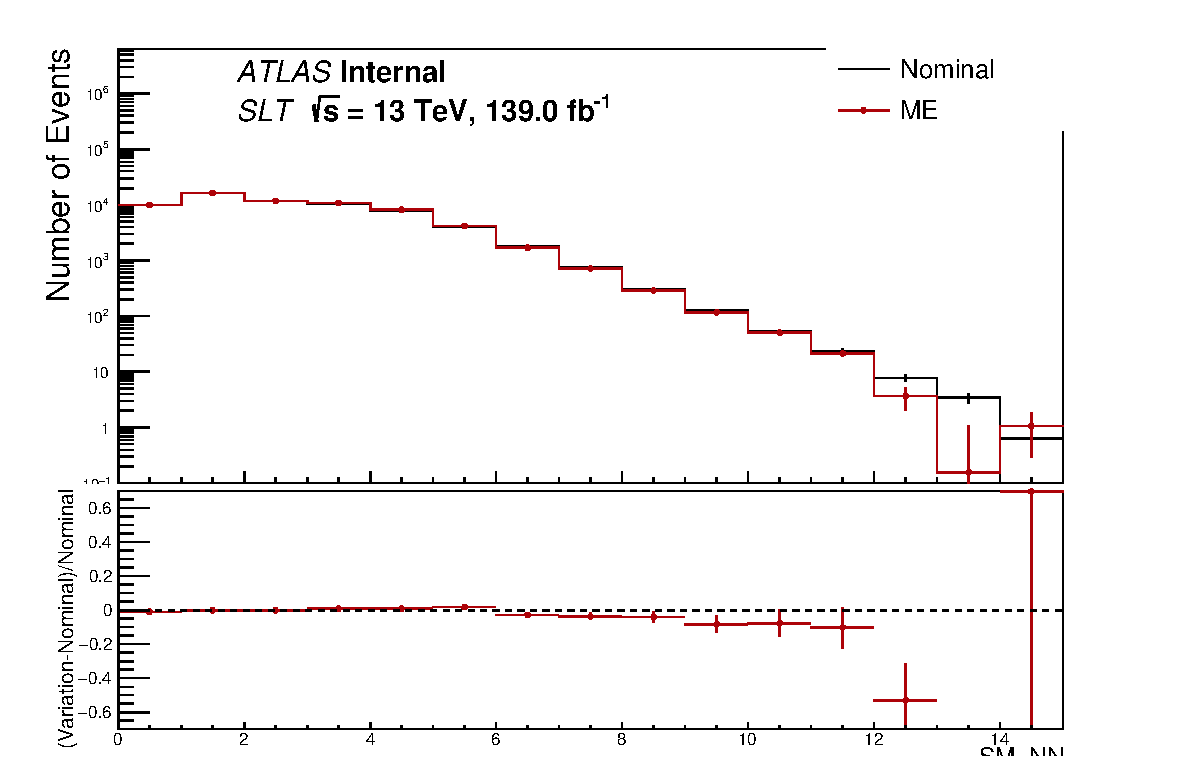
\includegraphics[width=.49\textwidth]{figures/lephad_modelling_systs/SLT/ME/limit_binning_SM_NN_Norm}
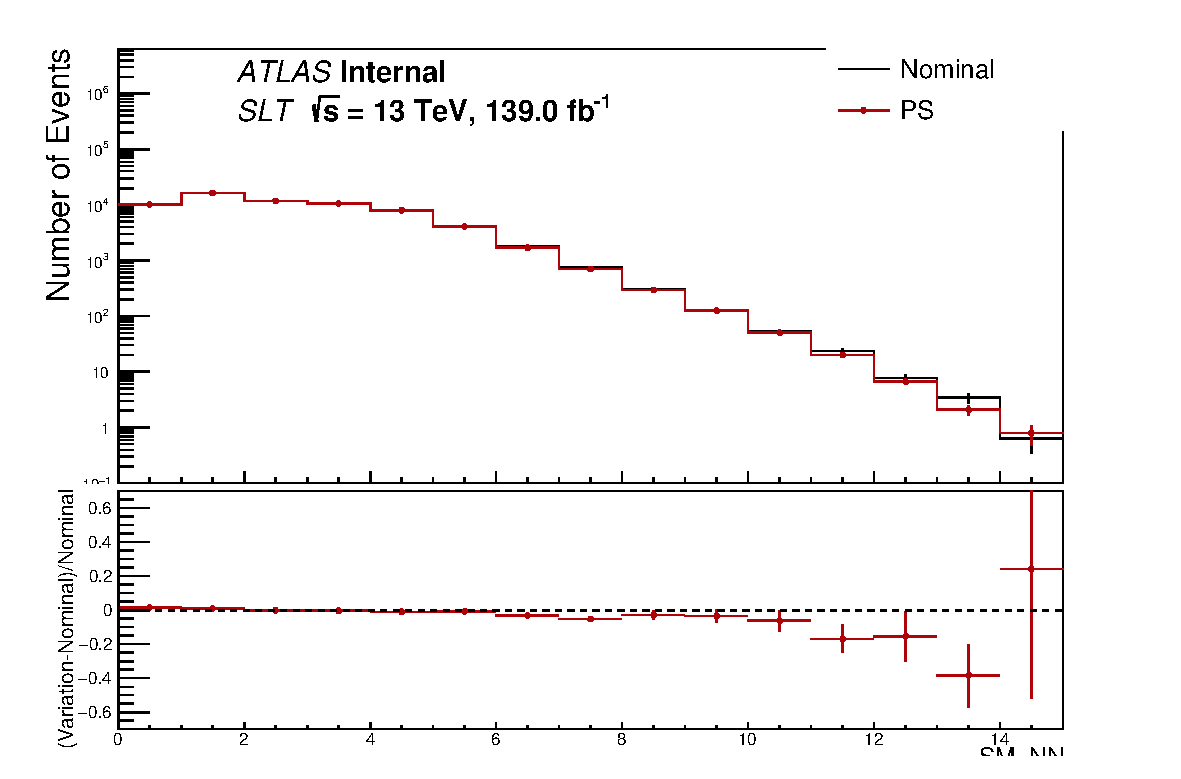
\includegraphics[width=.49\textwidth]{figures/lephad_modelling_systs/SLT/PS/limit_binning_SM_NN_Norm}\\
% 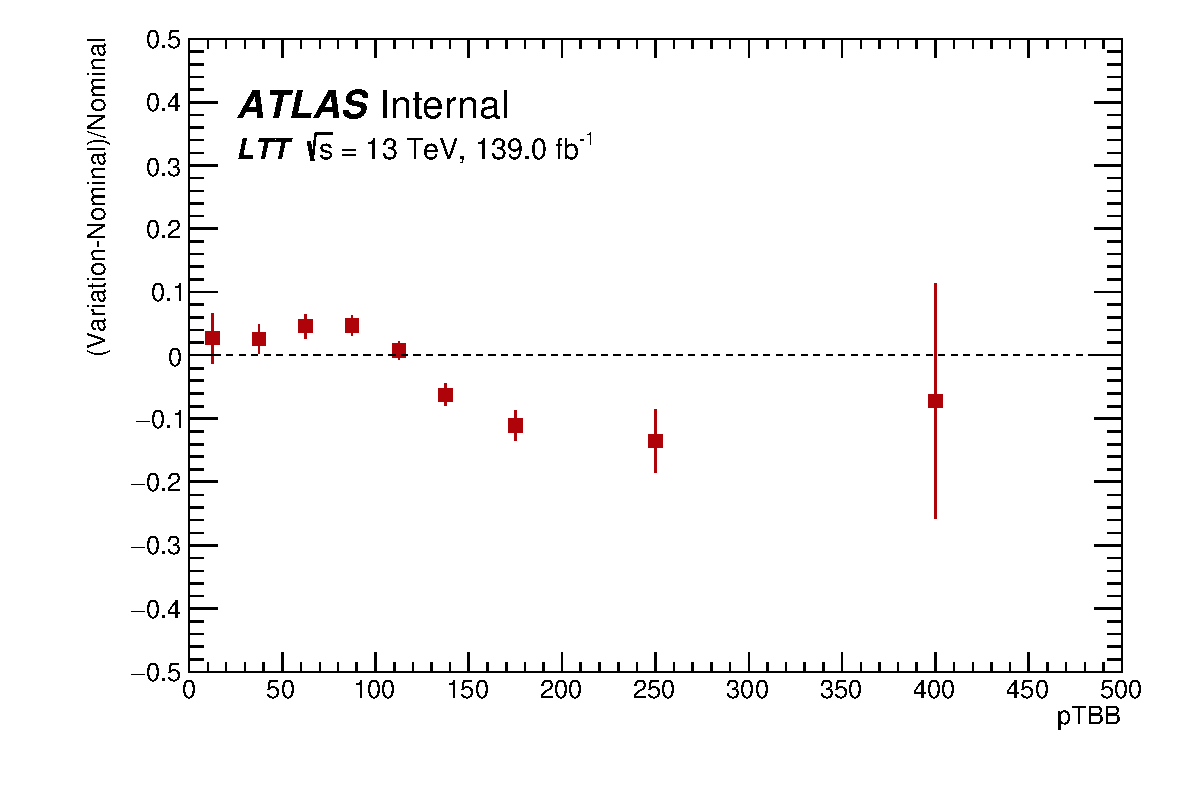
\includegraphics[width=.49\textwidth]{figures/lephad_modelling_systs/LTT/aMCNLO/pTBB_Norm}
% 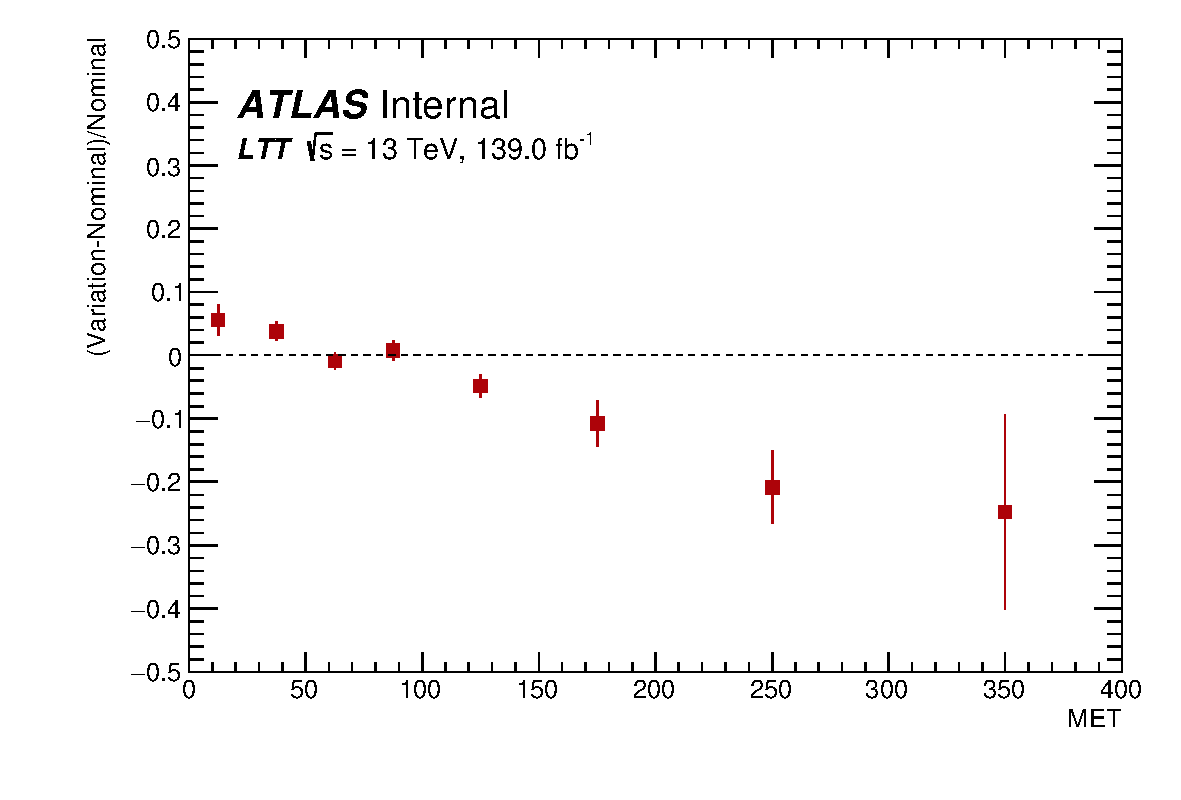
\includegraphics[width=.49\textwidth]{figures/lephad_modelling_systs/LTT/aMCNLO/MET_Norm}
\caption{Parametrisation in SM NN score distribution for the ME (left) and PS (right) systematics.}
\label{fig:ttbarsyst_lephad_SLT_NN}
\end{figure}


% \begin{figure}
%   \centering
%   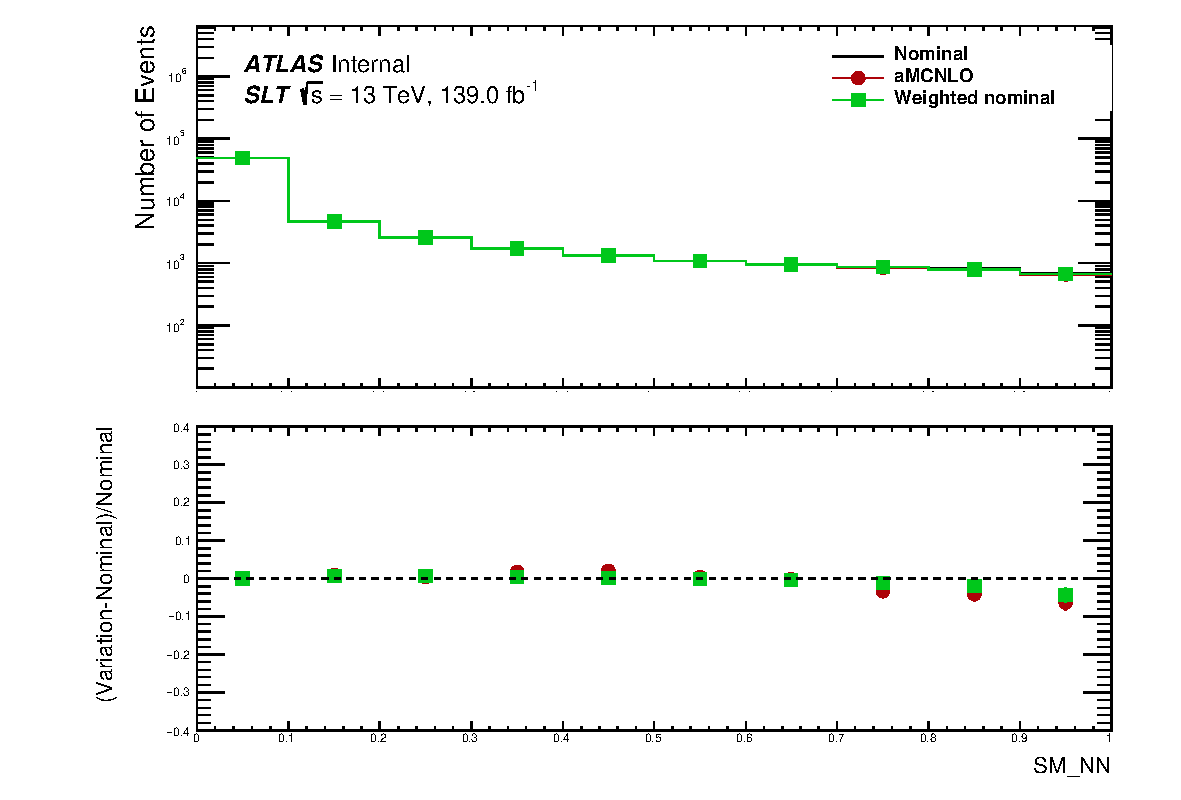
\includegraphics[width=.49\textwidth]{figures/lephad_modelling_systs/SLT/aMCNLO/Hist_and_ratio_SM_NN_Norm.png}
%   % 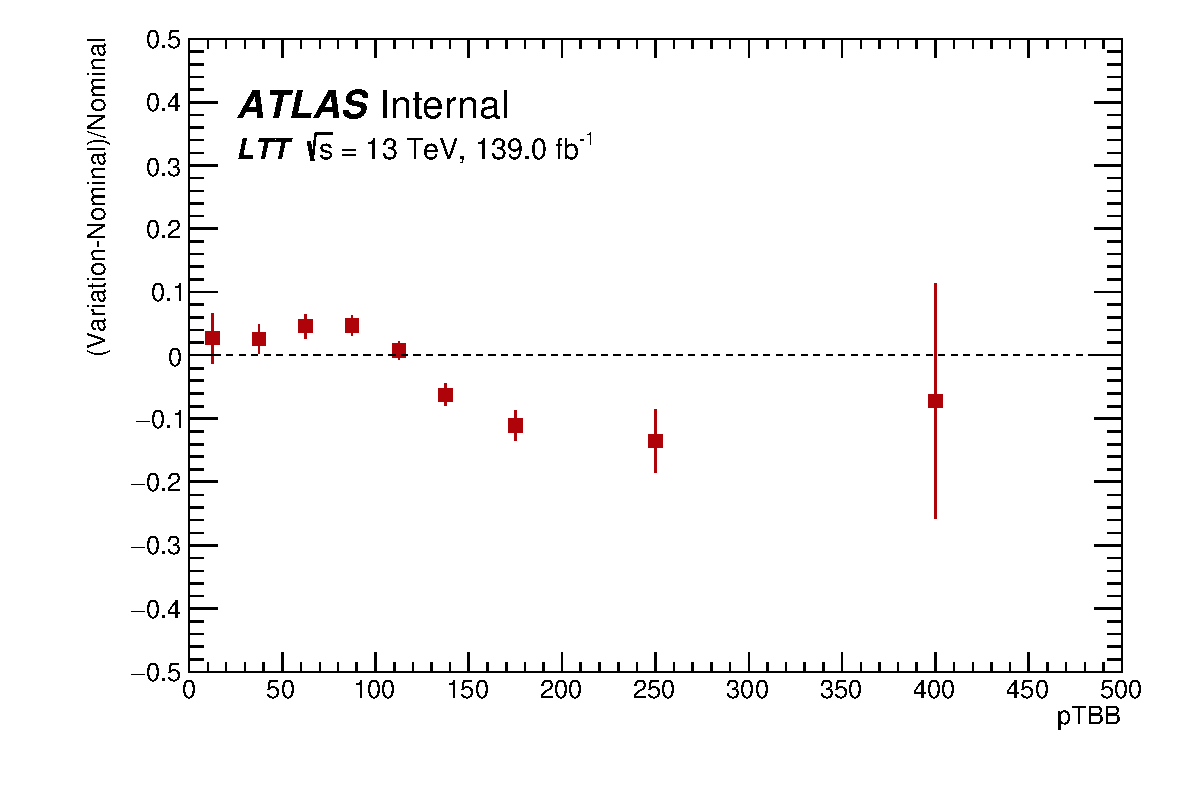
\includegraphics[width=.49\textwidth]{figures/lephad_modelling_systs/LTT/aMCNLO/pTBB_Norm.png}
%   % 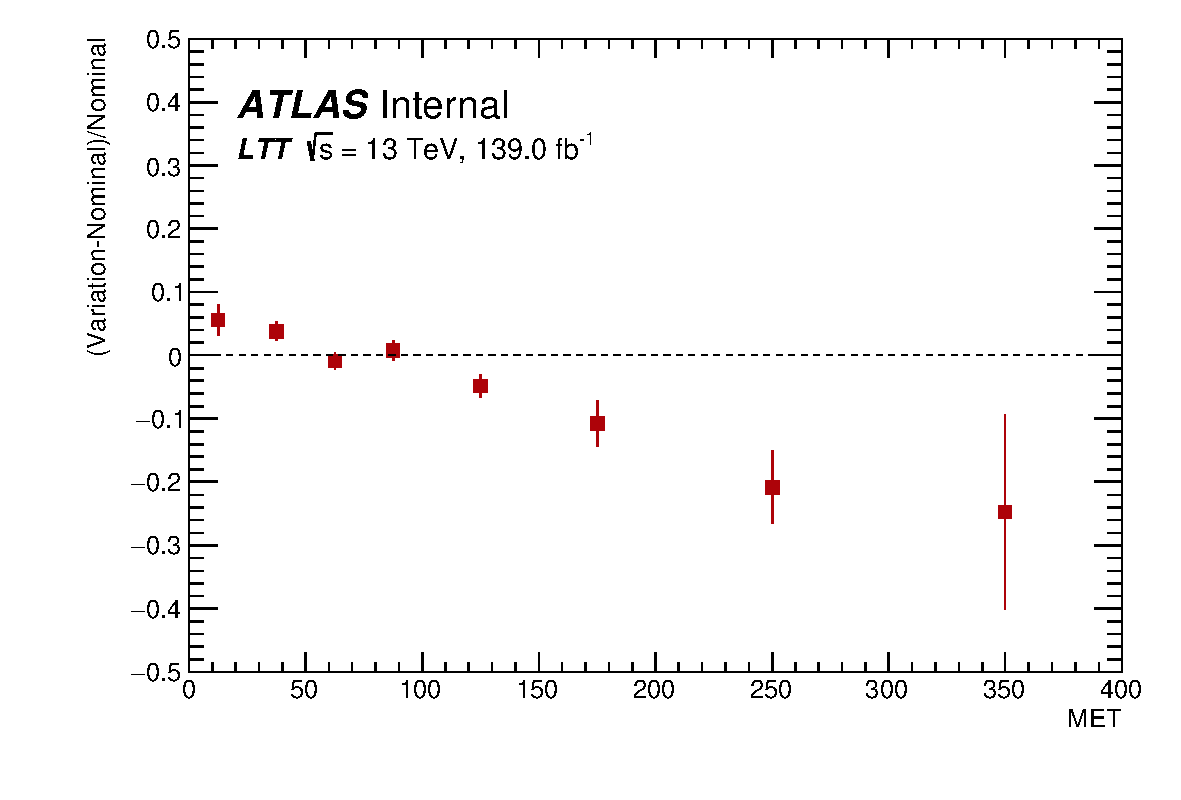
\includegraphics[width=.49\textwidth]{figures/lephad_modelling_systs/LTT/aMCNLO/MET_Norm.png}
%   \caption{SLT channel: shape-only NN score of the ME variation and the weighted nominal.}
%   \label{fig:ttbarsyst_lephad_amc_NN}
%   \end{figure}
  


%Parton shower hadronisation algorithmic uncertainties are evaluated comparing samples showered with Pythia8 versus Herwig7. 

% The parton shower uncertainty is parametrised similarly to the aMC 
% with a sequential parametrisation. The parametrisation is done first 
% in bins of the \pt\ of the subleading jet followed by parametrisation in bins
% of mass of the di-Higgs system, as shown in Fig.~\ref{fig:ttbarsyst_lephad_herwig}
% for the SLT channel. 
% The closure of the parametrisation in the NN score is shown in Fig.~\ref{fig:ttbarsyst_lephad_herwig_NN}.

% \begin{figure}
% 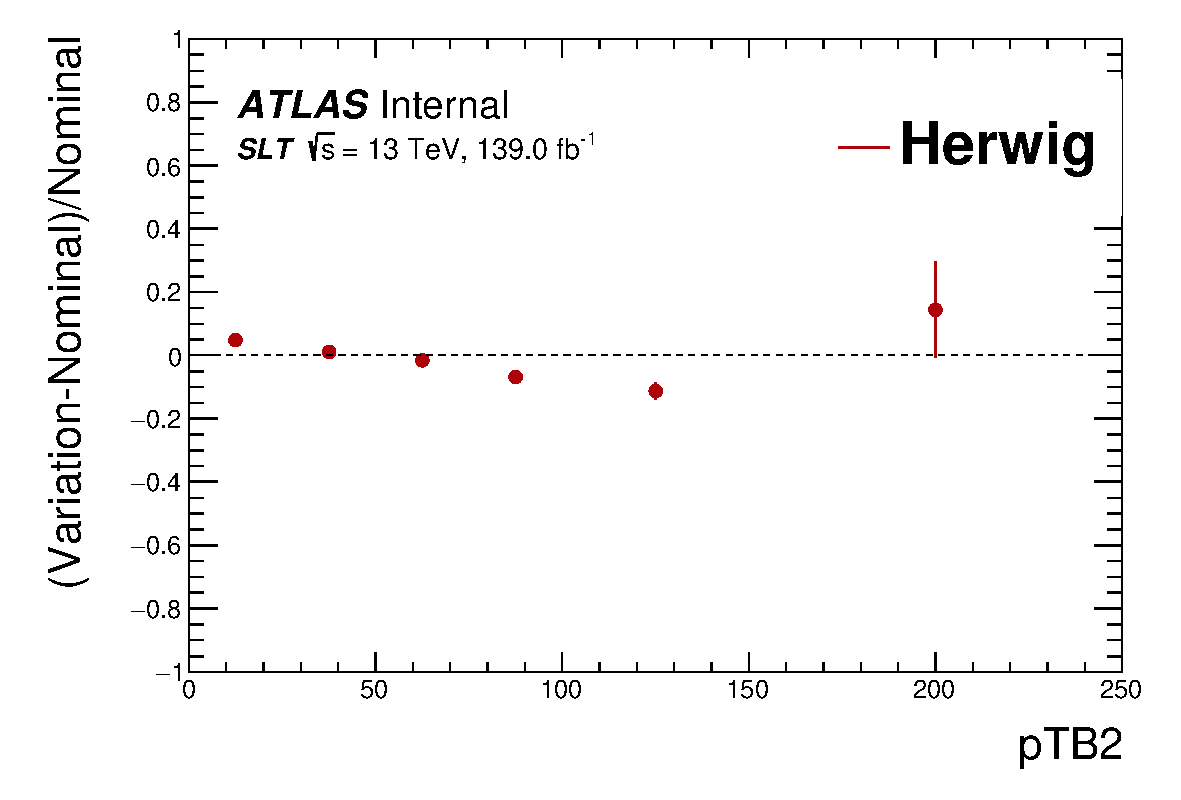
\includegraphics[width=.49\textwidth]{figures/lephad_modelling_systs/SLT/Herwig/pTB2_Norm.png}
% 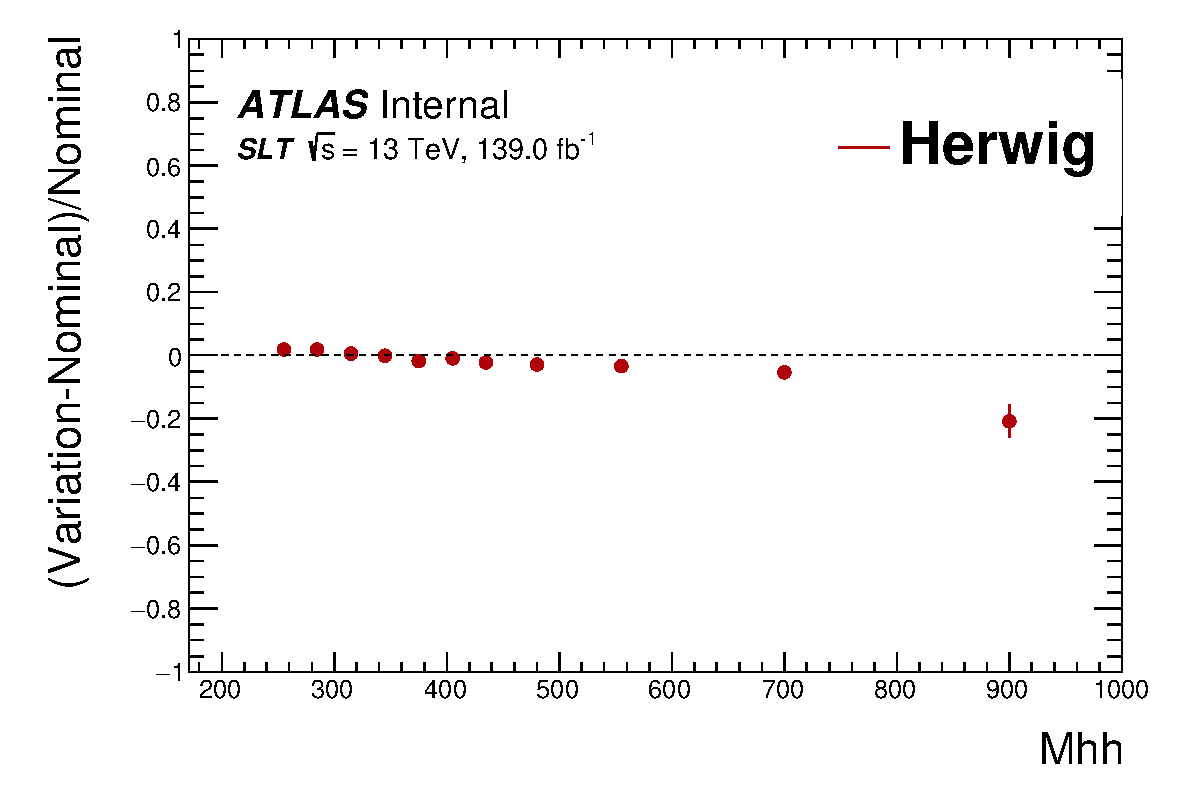
\includegraphics[width=.49\textwidth]{figures/lephad_modelling_systs/SLT/Herwig/Mhh_Norm.png}
% \caption{SLT: Parametrisation in bins of $p_T^{b2}$ distribution (left) and the $m_{HH}$ distribution
%  for the Herwig variation.}
% \label{fig:ttbarsyst_lephad_herwig}
% \end{figure}

% \begin{figure}
%   \centering
%   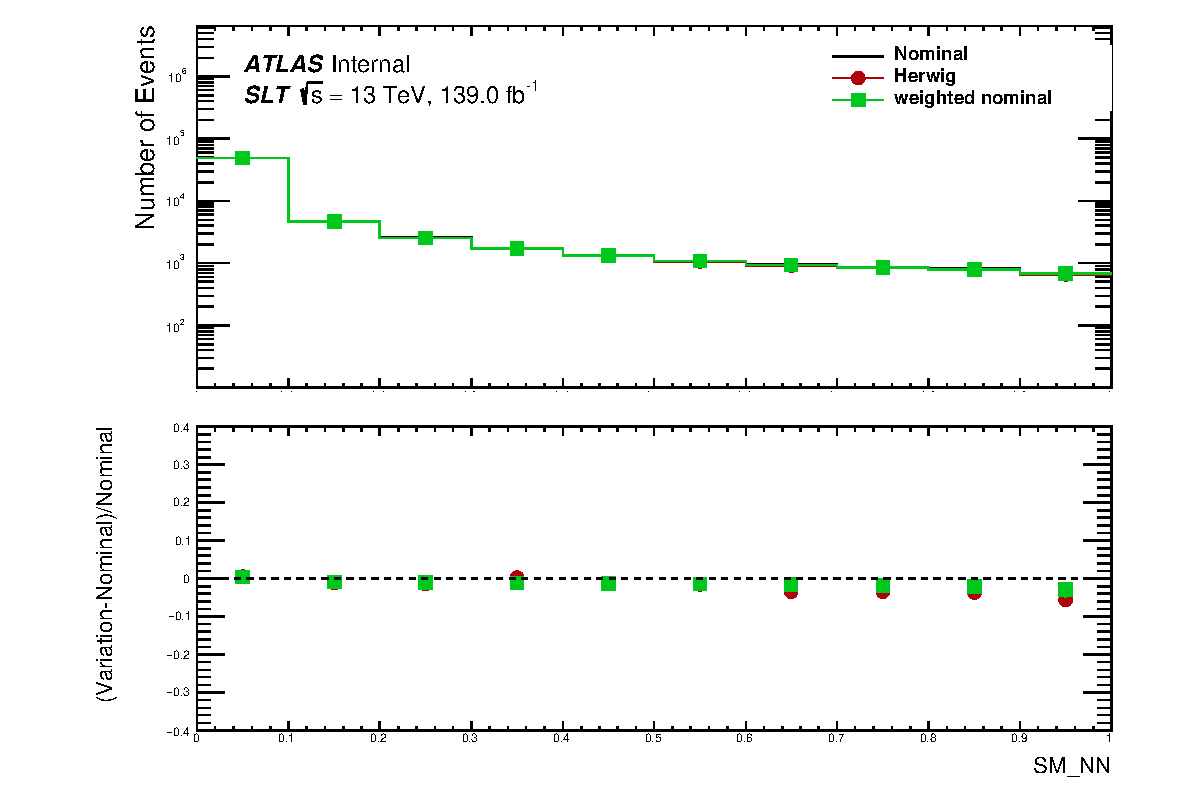
\includegraphics[width=.49\textwidth]{figures/lephad_modelling_systs/SLT/Herwig/Hist_and_ratio_SM_NN_Norm.png}
%   % 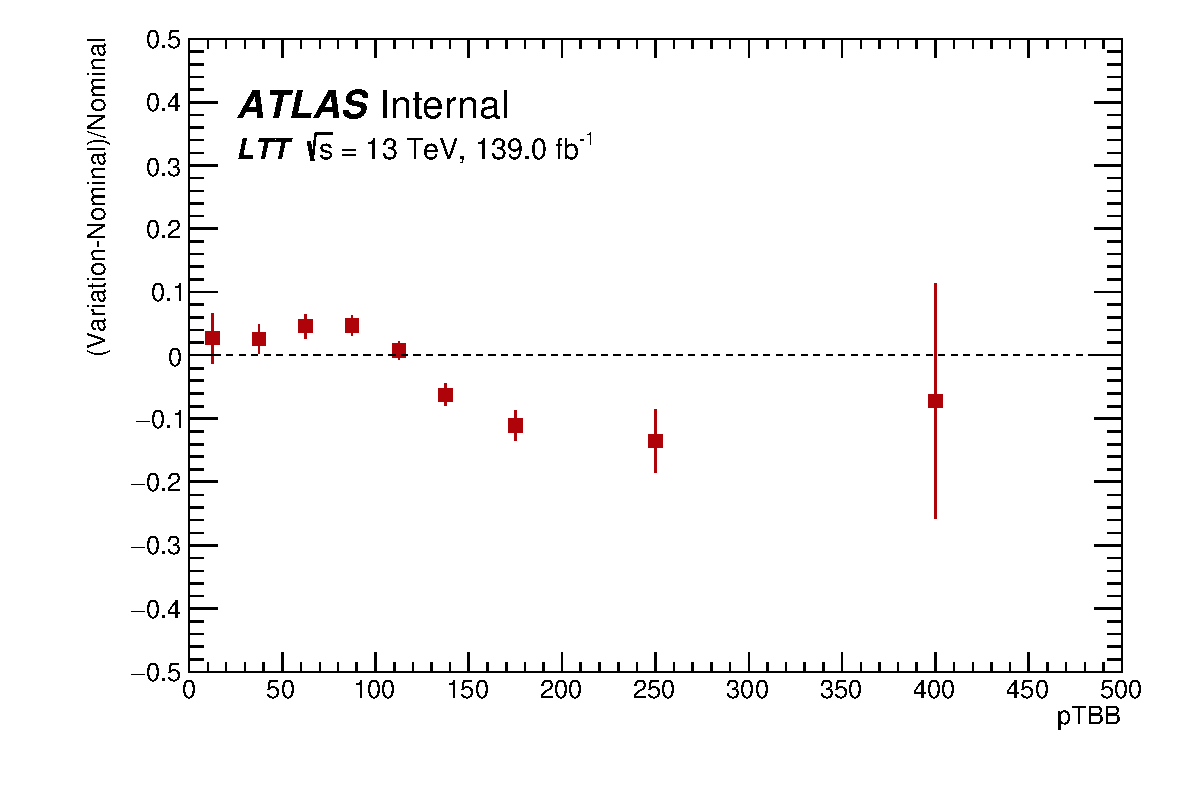
\includegraphics[width=.49\textwidth]{figures/lephad_modelling_systs/LTT/aMCNLO/pTBB_Norm.png}
%   % 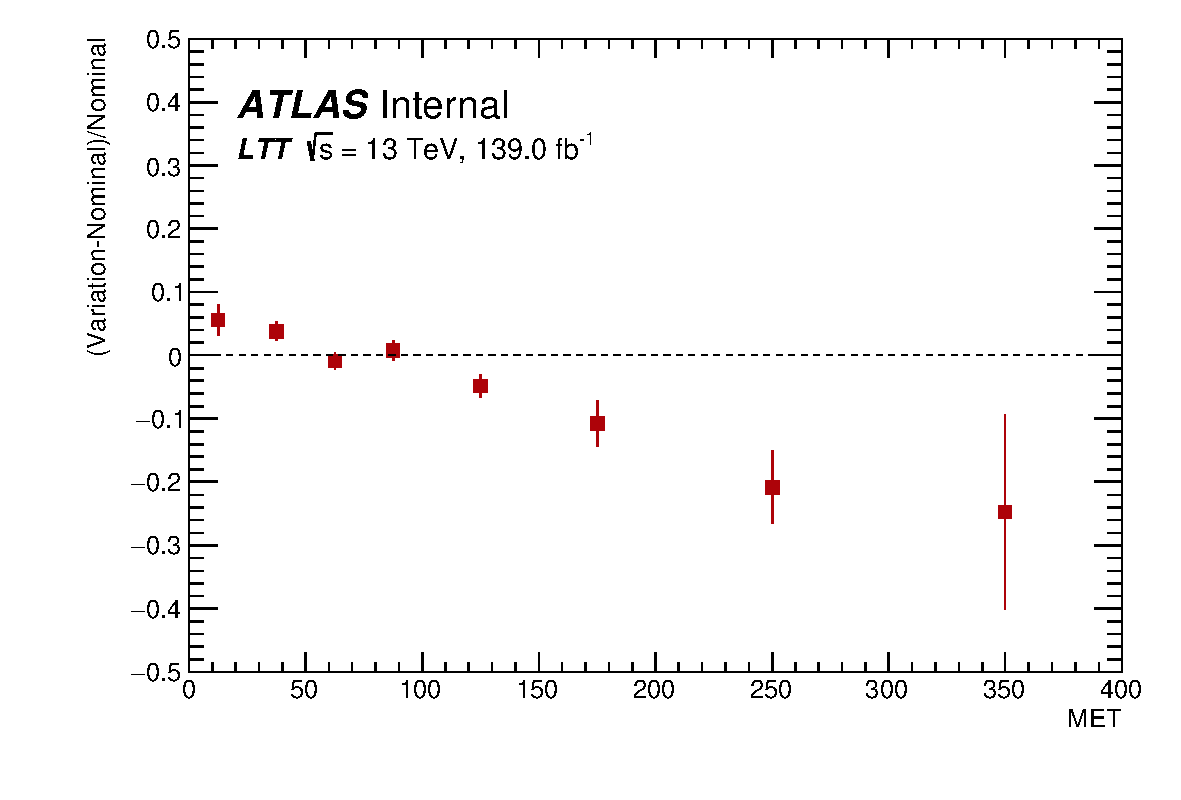
\includegraphics[width=.49\textwidth]{figures/lephad_modelling_systs/LTT/aMCNLO/MET_Norm.png}
%   \caption{SLT channel: shape-only NN score of the Herwig variation and the weighted nominal.}
%   \label{fig:ttbarsyst_lephad_herwig_NN}
%   \end{figure}
  

The ISR up and down variations have not shown obvious shape in the NN/PNN distribution 
therefore only normalisation uncertainty is considered. 
%  \begin{figure}
% \centering
% 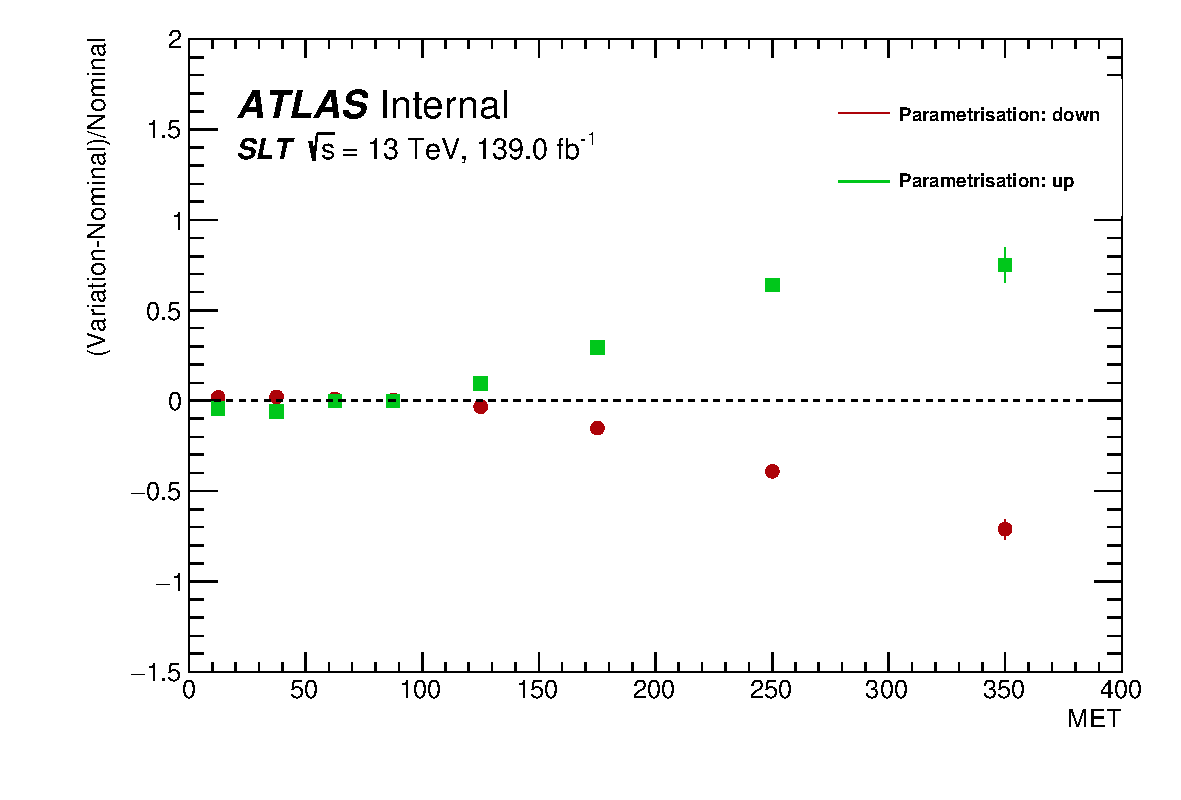
\includegraphics[width=.49\textwidth]{figures/lephad_modelling_systs/SLT/ISRlow/MET_Norm.png}
% 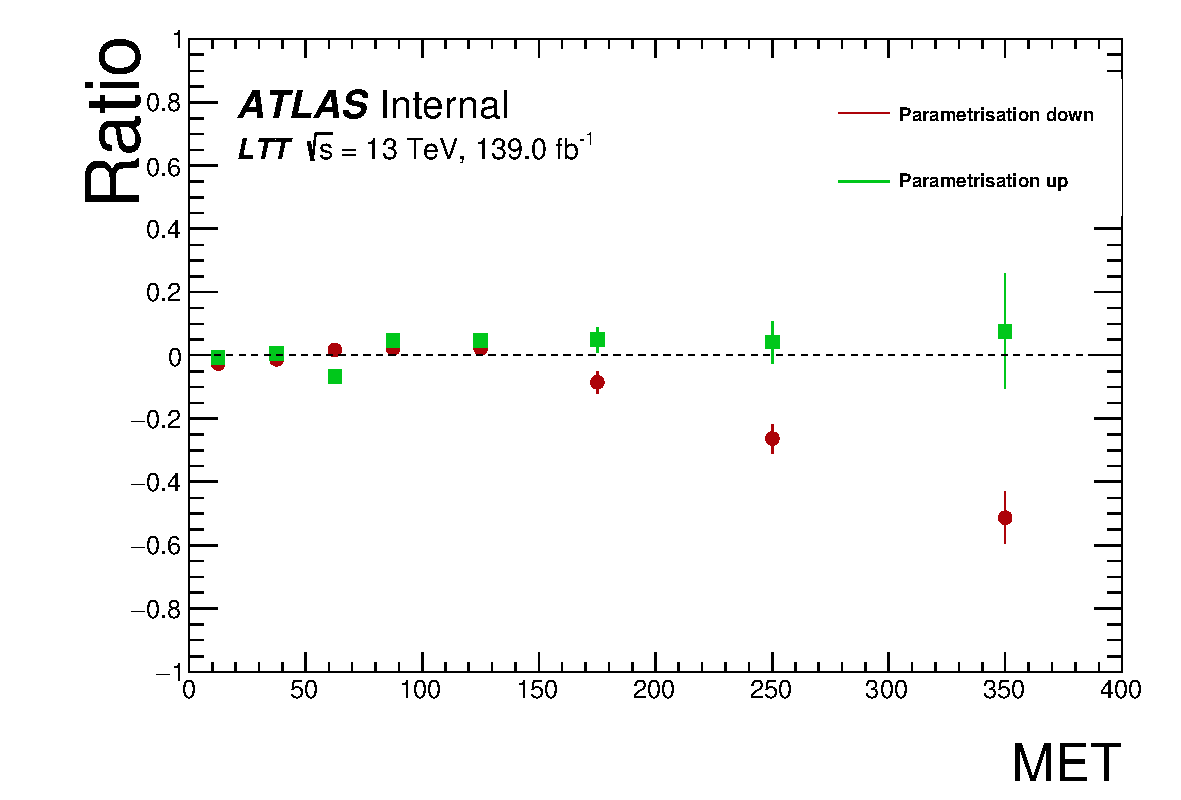
\includegraphics[width=.49\textwidth]{figures/lephad_modelling_systs/LTT/ISRlow/MET_Norm.png}
% \caption{SLT (left) and LTT channel (right): Parametrisation in bins of the MET distribution for the ISR variation.}
% \label{fig:ttbarsyst_lephad_isr_MET}
% \end{figure}





\paragraph{Uncertainties on $t\bar{t}$ in the \hadhad
  channel}\mbox{}\\

The shapes of two-point \ttbar modelling uncertainties (i.e.\ ME, PS
and ISR) are directly estimated by comparing the MVA discriminants of
the (fast-sim.) variation sample with the nominal (fast-sim.) \ttbar
sample. The shape differences are parametrized by taking the ratio of
the normalized variation histogram and the normalized nominal
histogram in bins of the MVA discriminant. This ratio is subsequently
applied as a multiplicative factor to the nominal \ttbar sample using
full simulation. To limit the impact of statistical fluctuations on
the variation template entering the fit, the binning of the ratio
parametrizing the shape is chosen such that about 5 \% of nominal
\ttbar populates each bin\footnote{The exact fraction can vary as the
  derivation is performed using pre-binned data using the same binning
  that is also used as the input to the rebinning algorithms used in
  the final fit. In extreme cases, e.g.\ for the high-mass PNN
  discriminants, where almost perfect discrimination between signal
  and \ttbar is possible the exact fraction can be significantly
  larger.}. This limits the statistical uncertainties on the weighting
factors describing the shape of the uncertainty to less than 3 \% and
allows for a good description of the bulk of \ttbar events.

In~\ref{fig:hadhad_ttbar_syst_parametrization} the parametrization of
the \ttbar ME, PS and ISR uncertainties is shown with respect to the
SM-BDT. The parametrization for all PNN distributions is done
analogously. The main difference of the PNN parametrization is that
for the PNN discriminants used to extract high-mass resonances, the
high MVA-score region is dominated by the Z+jets background and close
to perfect discrimination between signal and \ttbar discrimination is
possible. Therefore, \ttbar is concentrated in the first bin of the
fitted distributions leading to no sensitivity to shape differences of
the MVA distribution for \ttbar.

\begin{figure}[htbp]
  \centering

  \subfloat[]{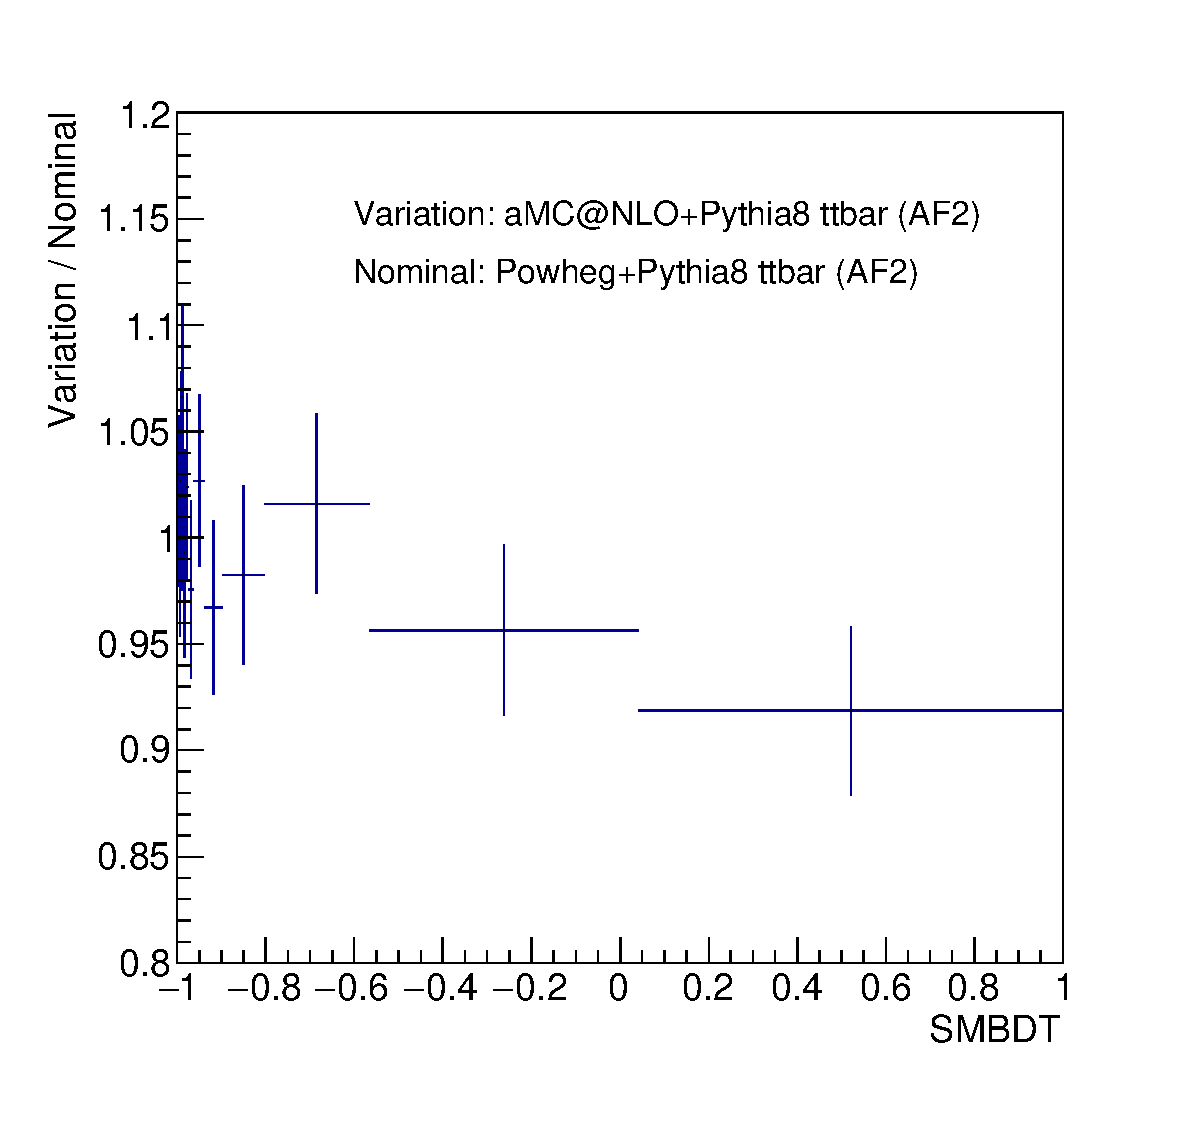
\includegraphics[width=0.33\textwidth]{figures/systs/hadhad_ttbar/hadhad_ttbar_me_mvaparam_SMBDT}}
  \subfloat[]{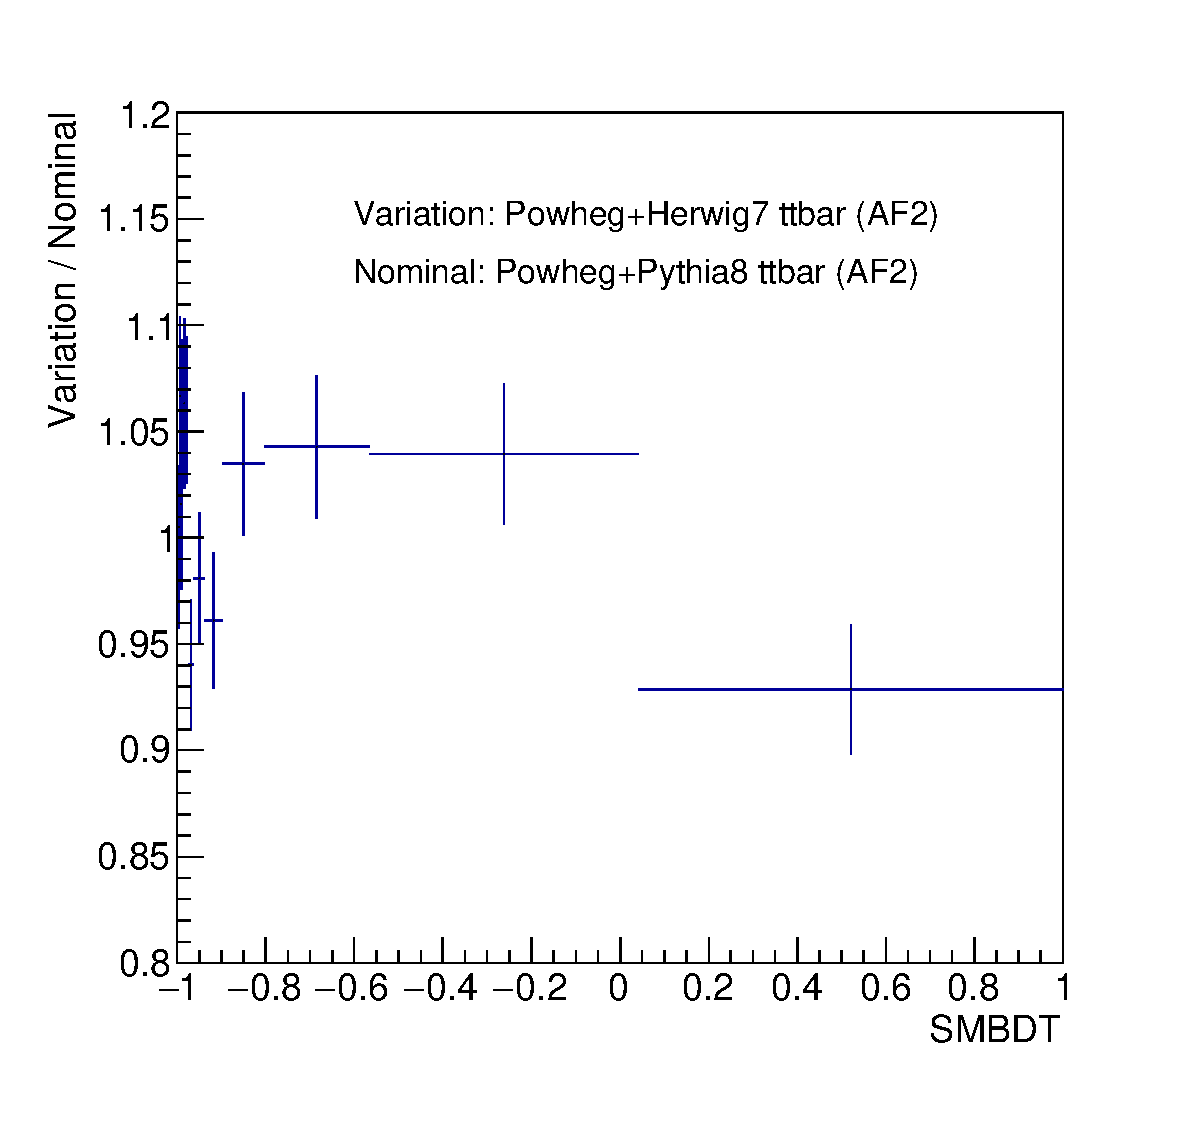
\includegraphics[width=0.33\textwidth]{figures/systs/hadhad_ttbar/hadhad_ttbar_ps_mvaparam_SMBDT}}
  \subfloat[]{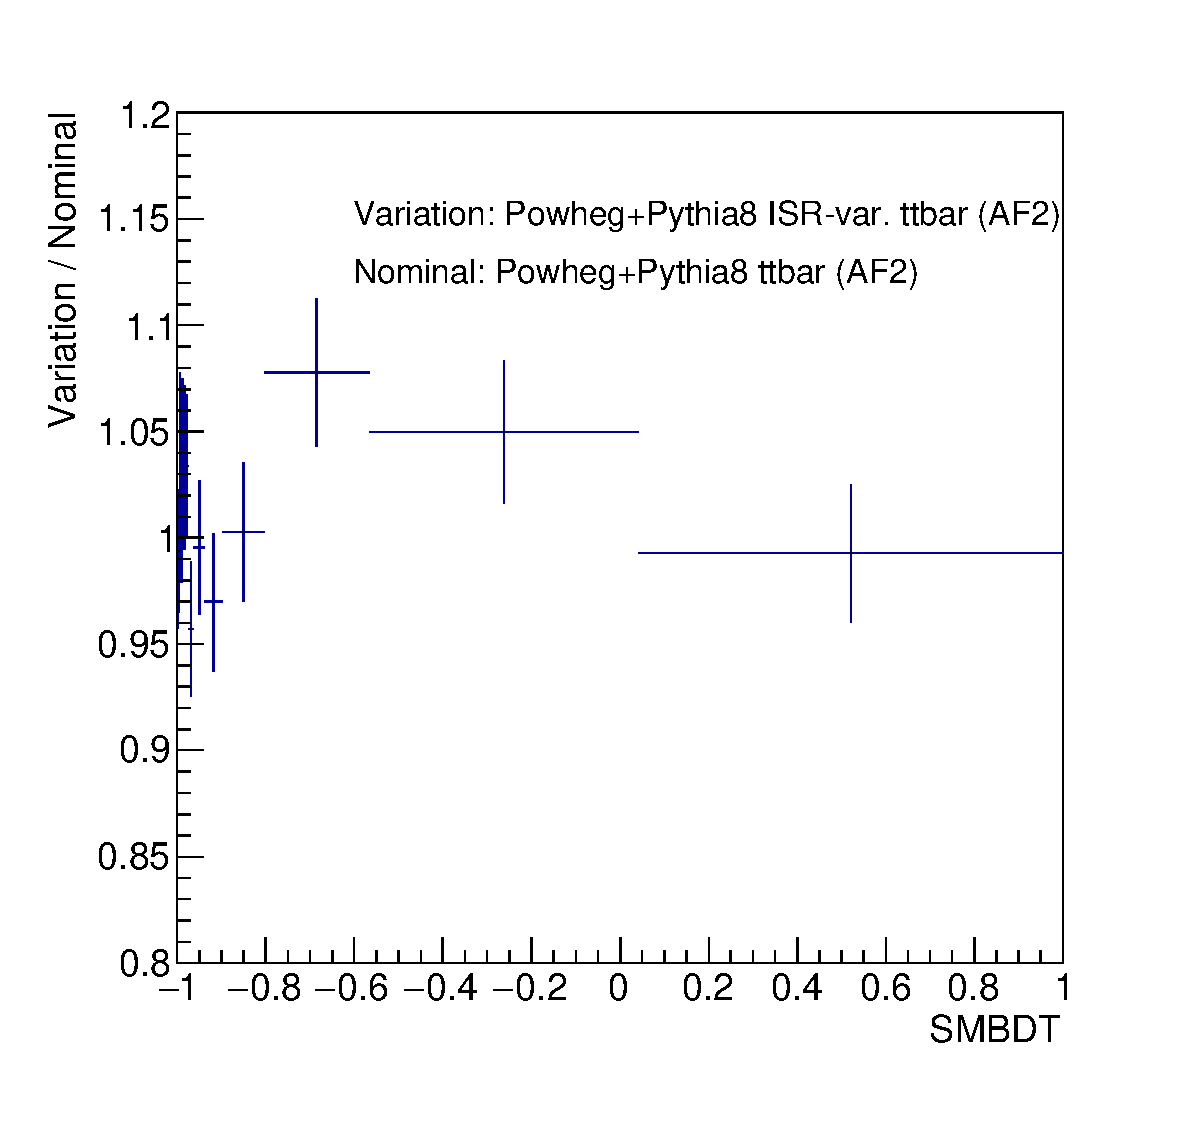
\includegraphics[width=0.33\textwidth]{figures/systs/hadhad_ttbar/hadhad_ttbar_isr_mvaparam_SMBDT}}

  \caption{Parametrization of the generator (a), parton shower (b) and
    ISR uncertainty (c) for the SMBDT distribution.}
  \label{fig:hadhad_ttbar_syst_parametrization}
\end{figure}

In~\ref{fig:hadhad_ttbar_syst_closure} the closure of the
parametrized uncertainties is shown for the SMBDT. The full set of all
relevant distributions is shown
in~\ref{subsec:appendix_systs_ttbarsysts_hadhad}.


\begin{figure}[htbp]
  \caption{Closure check of parametrized \ttbar uncertainties in the
    \hadhad channel for the generator (ME), parton shower (PS) and ISR
    uncertainty. The binning used for the closure check is the same as
    used for the final signal extraction fit. Note: The x-axis does
    not directly correspond to what is shown 
    in~\ref{fig:hadhad_ttbar_syst_parametrization} but uses the
    convention used for the final fit.}
  \label{fig:hadhad_ttbar_syst_closure}
\end{figure}

% Due to poor statistical precision of samples used for estimating \ttbar
% modelling uncertainties at high MVA score in $\tauhad\tauhad$, shape
% uncertainties are parametrised in other observables of the event and
% subsequently applied to the nominal \ttbar sample.

% The variation of the matrix element is parametrised in bins of the \pT of the
% \ttbar system. Residual variations (after \pT-\ttbar reweighting) are then
% evaluated in bins of the \pT of the subleading top. The parametrisation is shown
% in~\ref{fig:ttbarsyst_hadhad_me}.

% \begin{figure}
%   \centering
% 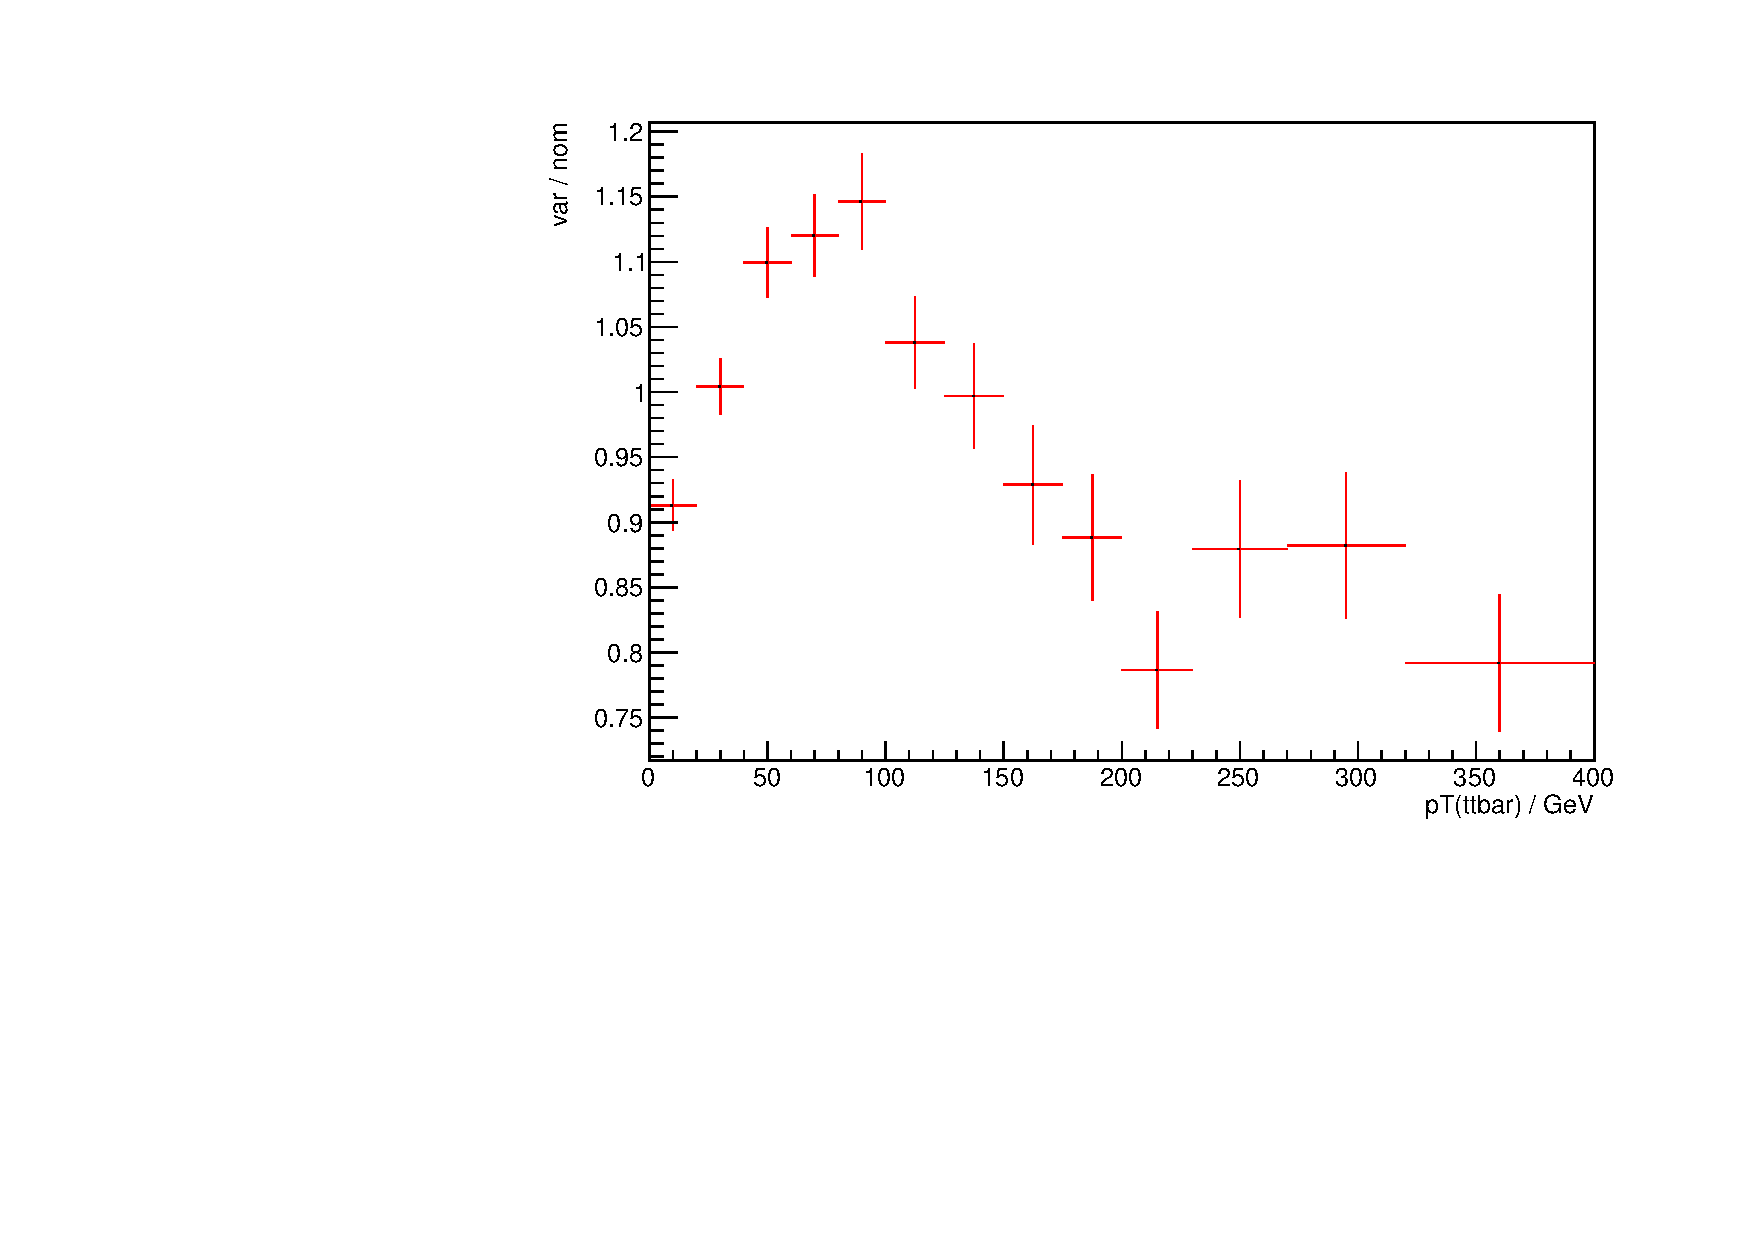
\includegraphics[width=0.49\textwidth]{figures/systs/hadhad_ttbar/me_ttbarpt}
% 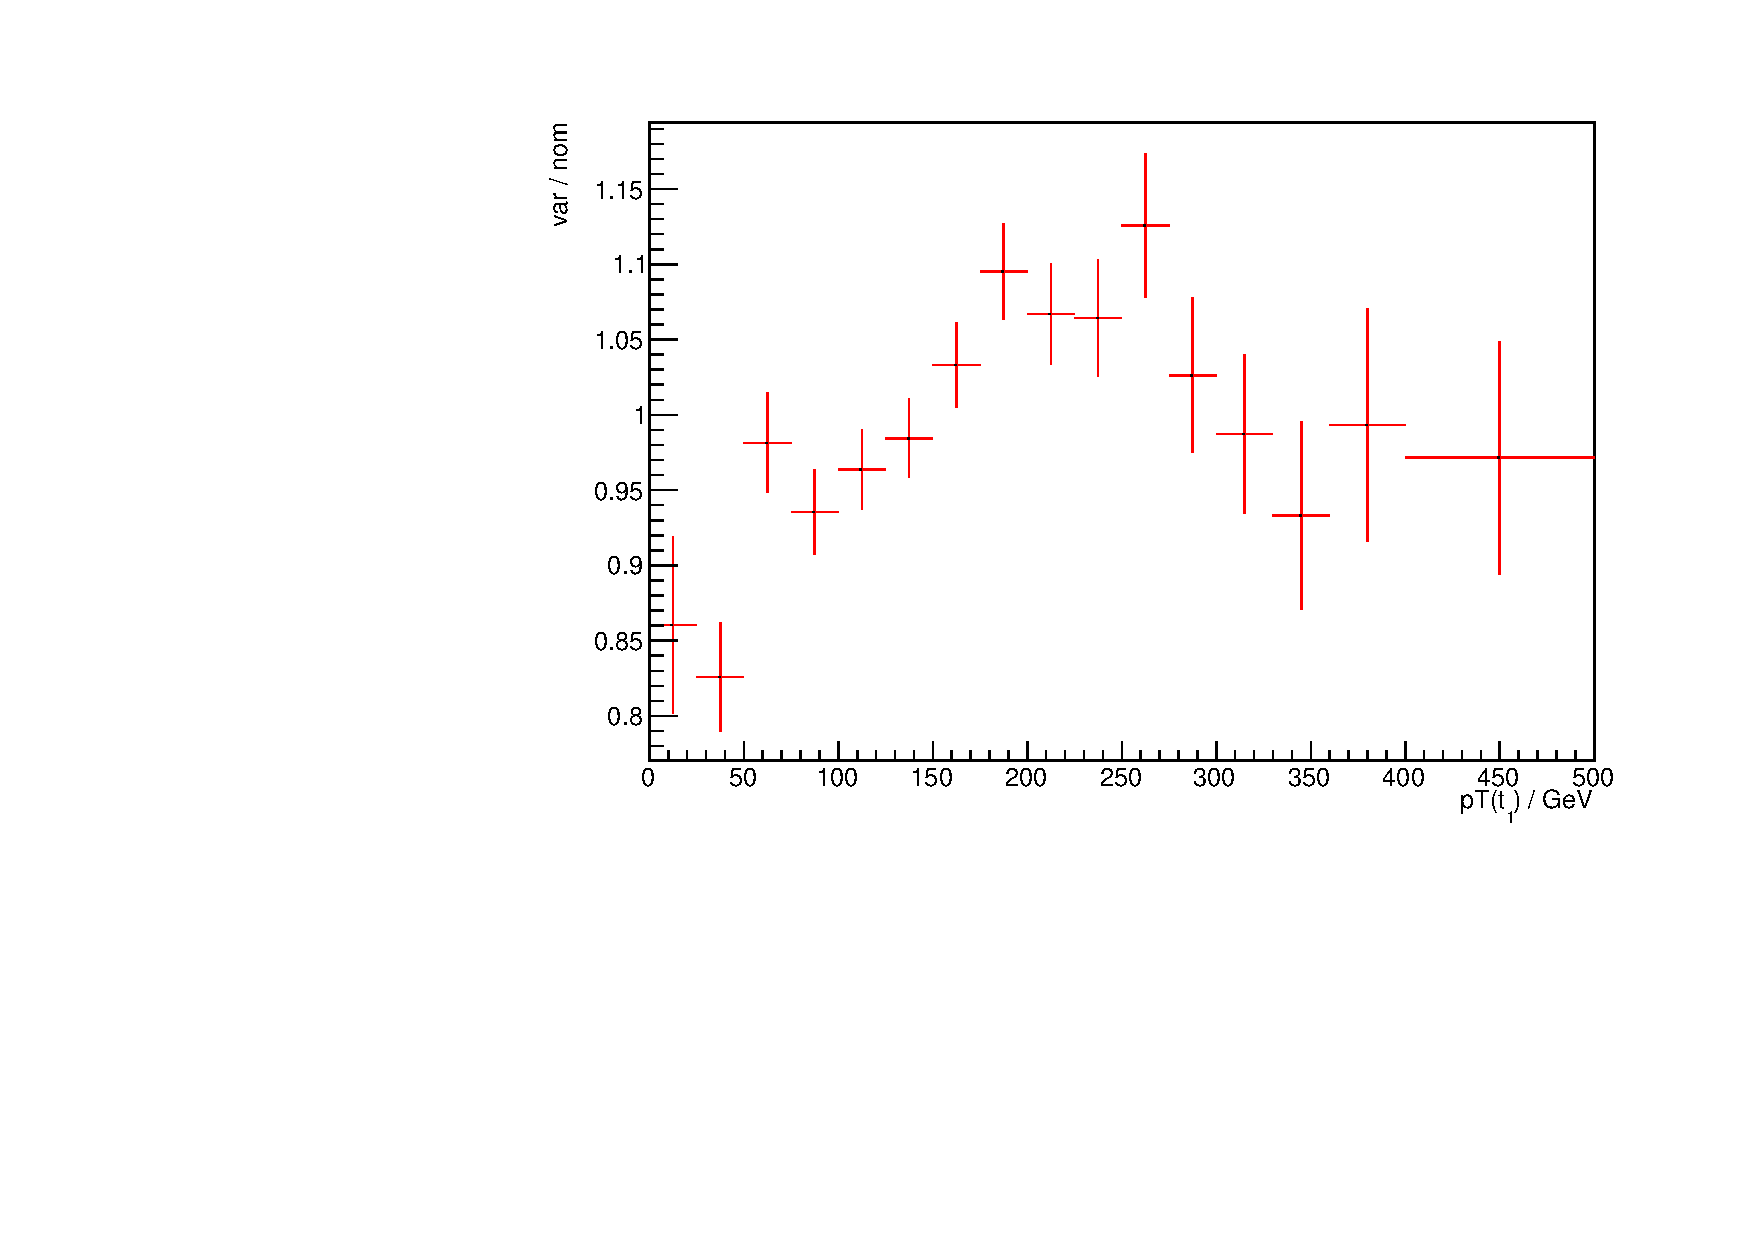
\includegraphics[width=0.49\textwidth]{figures/systs/hadhad_ttbar/me_toppt}
%   \caption{Parametrisation of the matrix element uncertainty (aMCAtNLO) in
%     $\tauhad\tauhad$. The ratio of variation and nominal yield is parametrised in bins of truth
%     \pT of the \ttbar system and truth \pT of the subleading top.}
%   \label{fig:ttbarsyst_hadhad_me}
% \end{figure}

% Similarly, the uncertainty due to the choice of parton shower is estimated by
% comparing Herwig7 with Pythia8. The uncertainty is parametrised sequentially in
% the leading and subleading b-jet \pT without applying any b-jet energy
% corrections. The parametrisation is shown in Figure~\ref{fig:ttbarsyst_hadhad_ps}.



% \begin{figure}
%   \centering
% 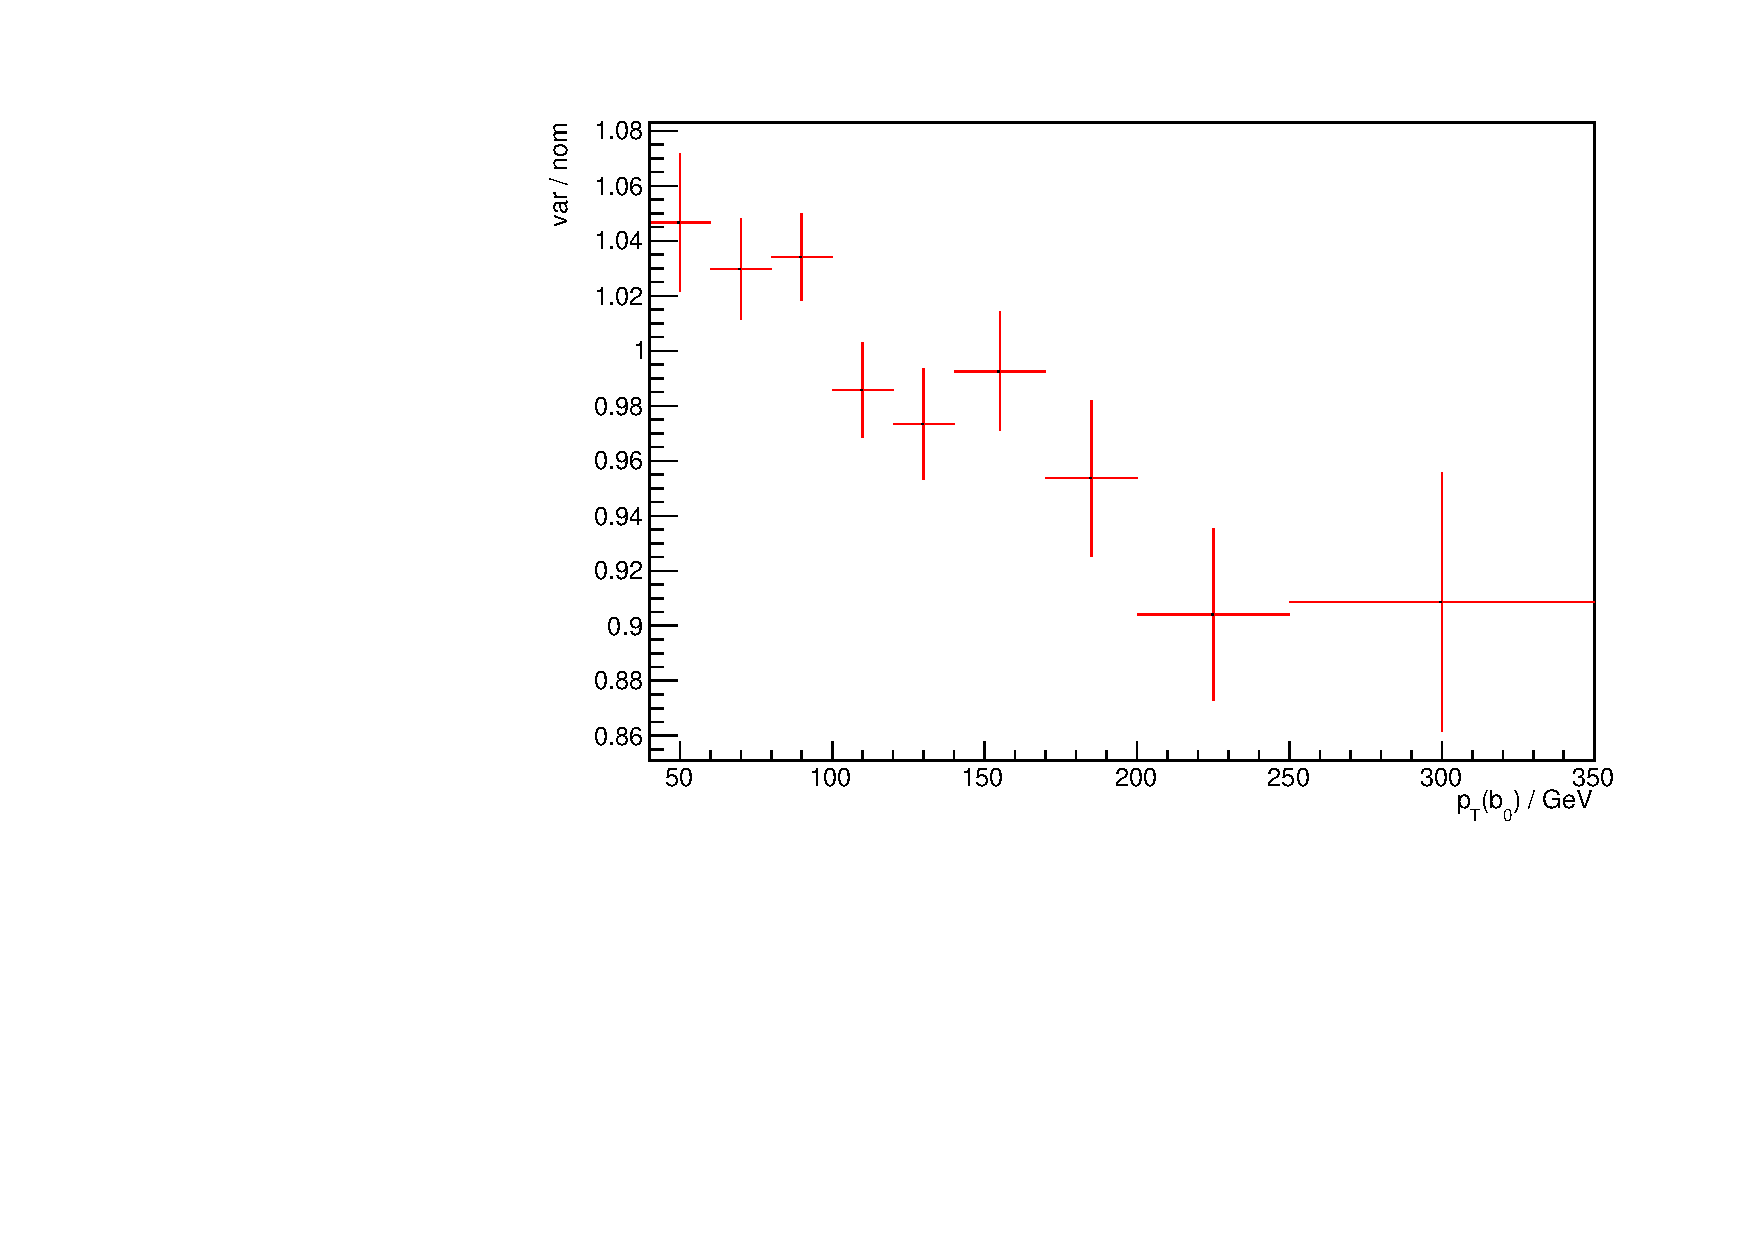
\includegraphics[width=0.49\textwidth]{figures/systs/hadhad_ttbar/ps_b0pt}
% 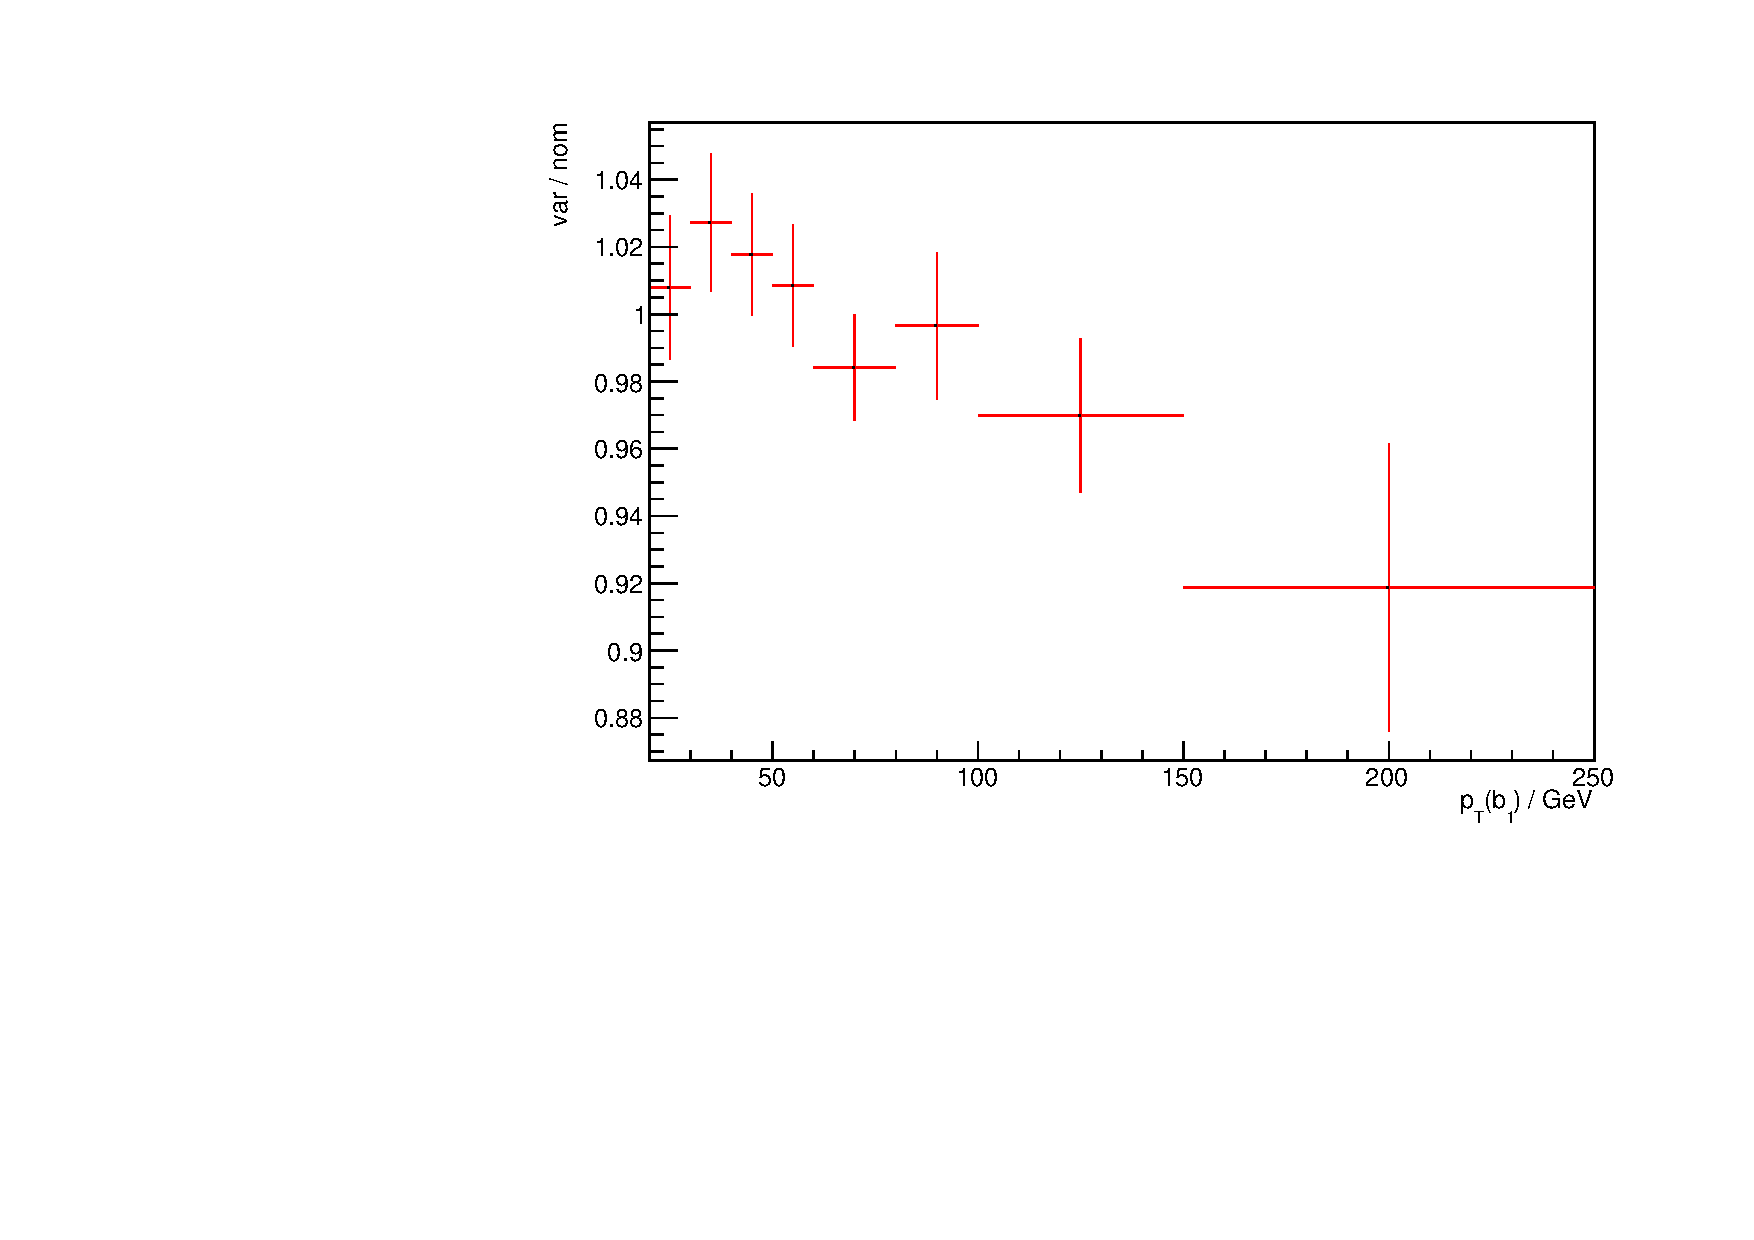
\includegraphics[width=0.49\textwidth]{figures/systs/hadhad_ttbar/ps_b1pt}
%   \caption{Parametrisation of the parton shower uncertainty (Herwig7) in
%     $\tauhad\tauhad$. The ratio of variation and nominal yield is parametrised in bins fo leading
%     and subleading b-jet \pT (before b-jet corrections).}
%   \label{fig:ttbarsyst_hadhad_ps}
% \end{figure}

% The modelling uncertainty due to initial state radiation is sequentially
% parametrized in the number of jets at truth-level with at least $\pT >
% \SI{20}{\GeV}$ and the \pT of the \ttbar-system. The parametrisation is shown in Figure~\ref{fig:ttbarsyst_hadhad_isr}.

% \begin{figure}
%   \centering
% 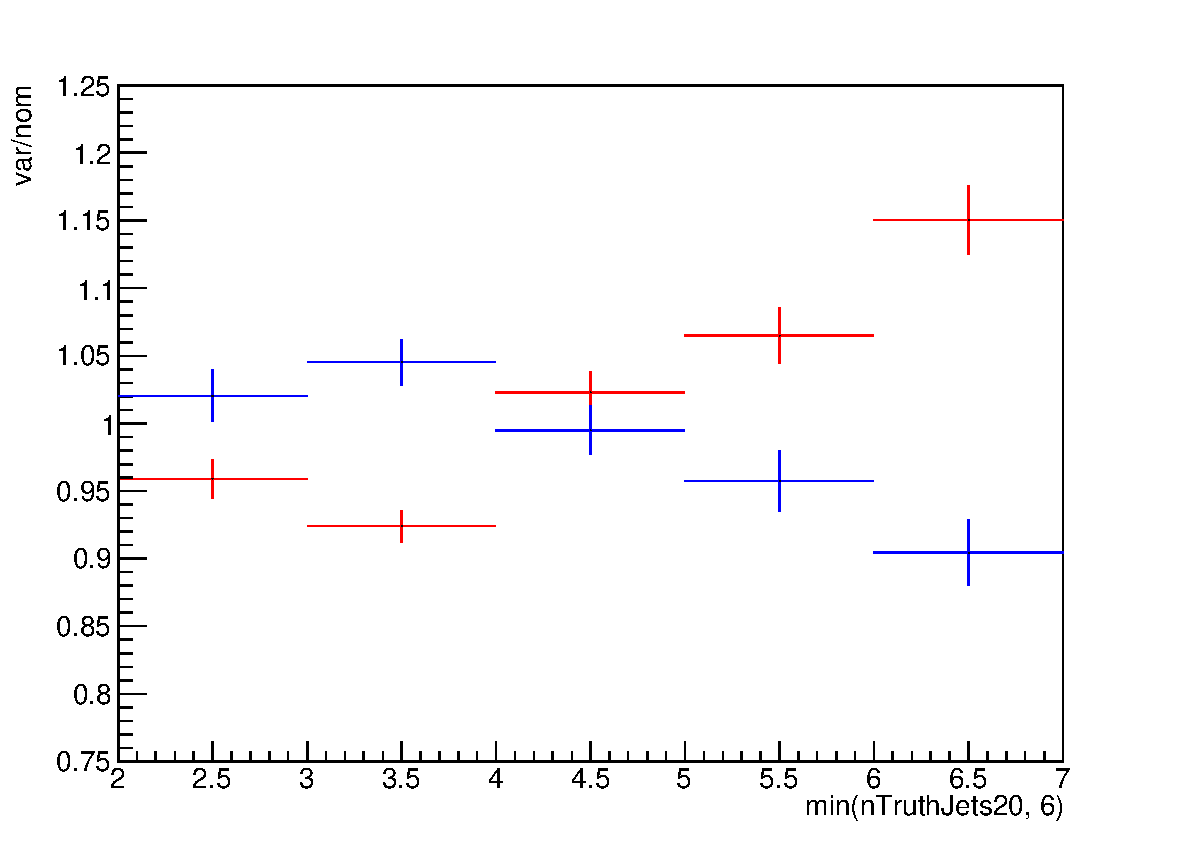
\includegraphics[width=0.49\textwidth]{figures/systs/hadhad_ttbar/isr_njets}
% 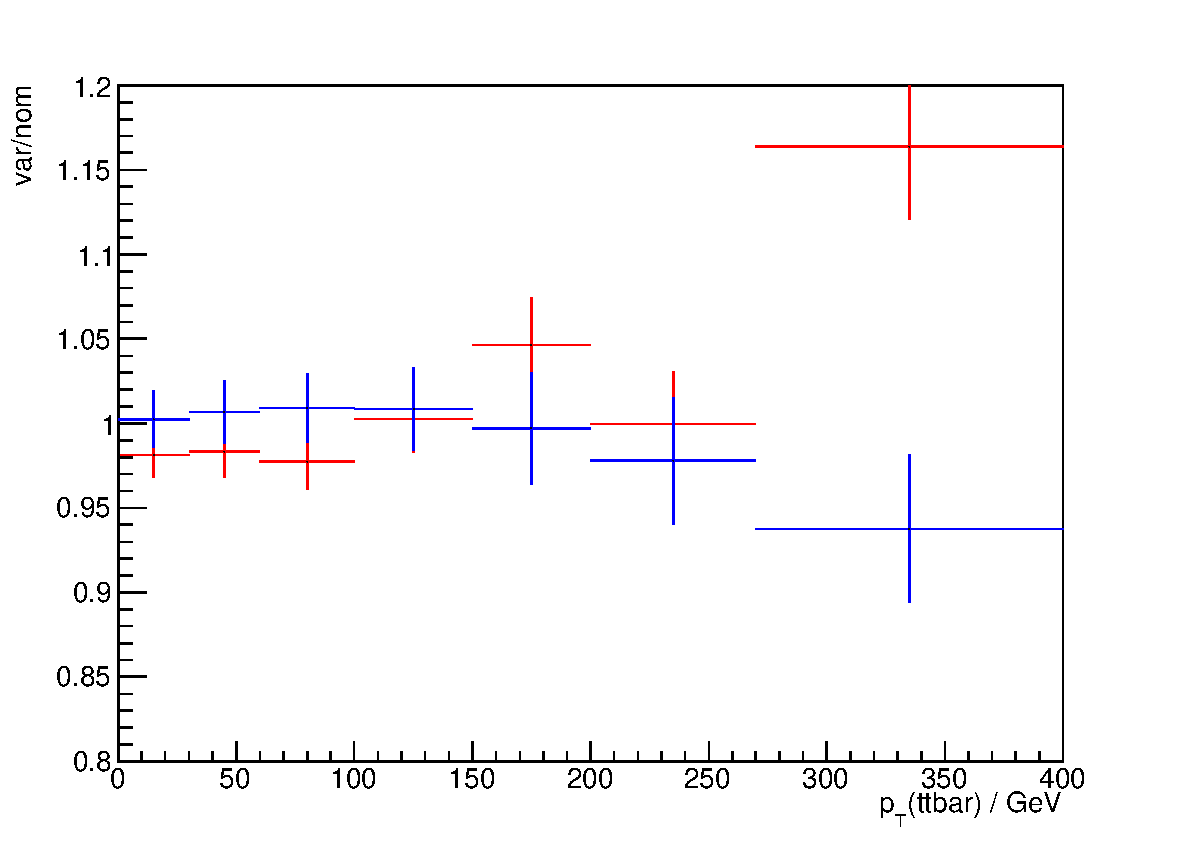
\includegraphics[width=0.49\textwidth]{figures/systs/hadhad_ttbar/isr_ttbarpt}
%   \caption{Parametrisation of the ISR uncertainty in $\tauhad\tauhad$ (up
%     variation in red, down variation in blue). The ratio
%   of variation and nominal yield is parametrised in bins of the number of truth
%   jets ($\pT > \SI{20}{\GeV}$) and \pT of the \ttbar system.}
%   \label{fig:ttbarsyst_hadhad_isr}
% \end{figure}

% The validity of the above parametrisations is examined by applying the
% parametrisation on the nominal \ttbar sample and comparing the MVA-score
% distributions used for signal extraction between the reweighted nominal and the
% variation. An exemplary closure check for the \SI{500}{\GeV} PNN-score
% distribution can be found in~\ref{fig:ttbarsyst_hadhad_closure}.

% \begin{figure}
%   \centering
% 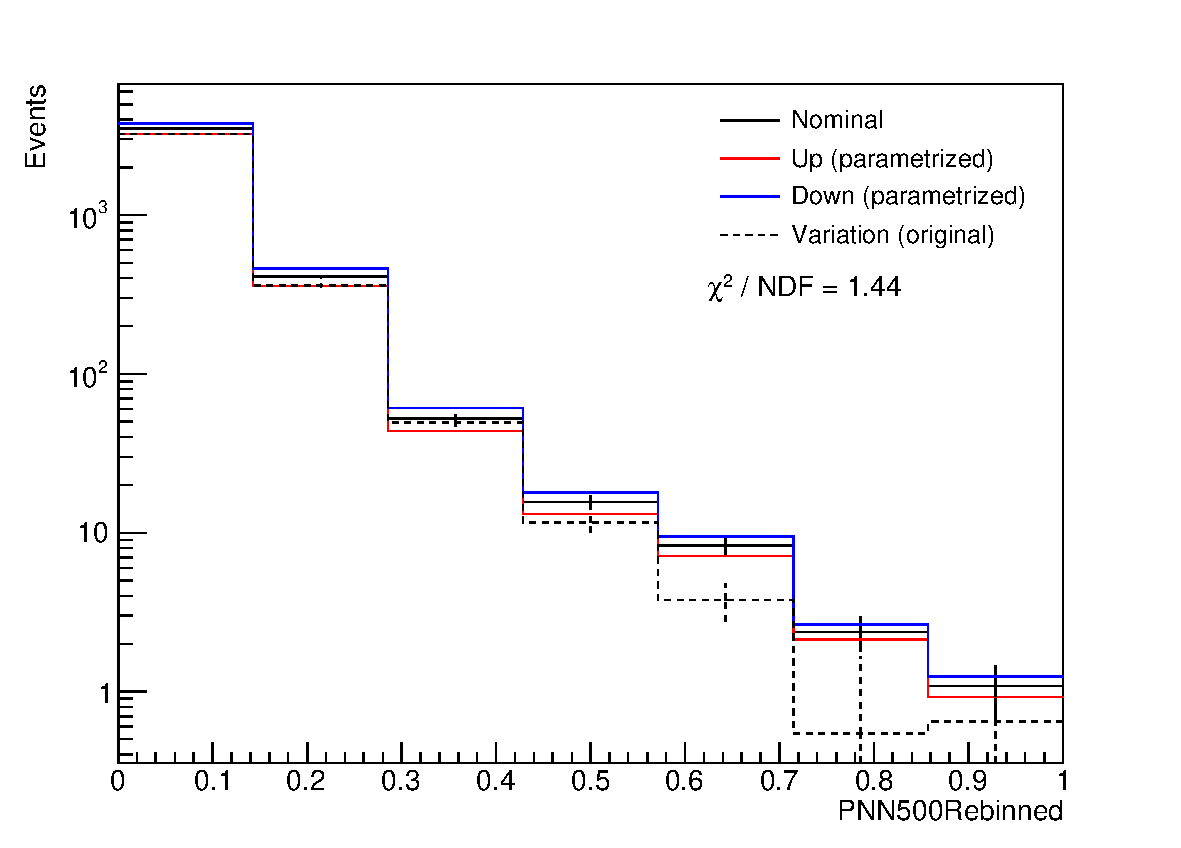
\includegraphics[width=0.32\textwidth]{figures/systs/hadhad_ttbar/gen_pnn500}
% 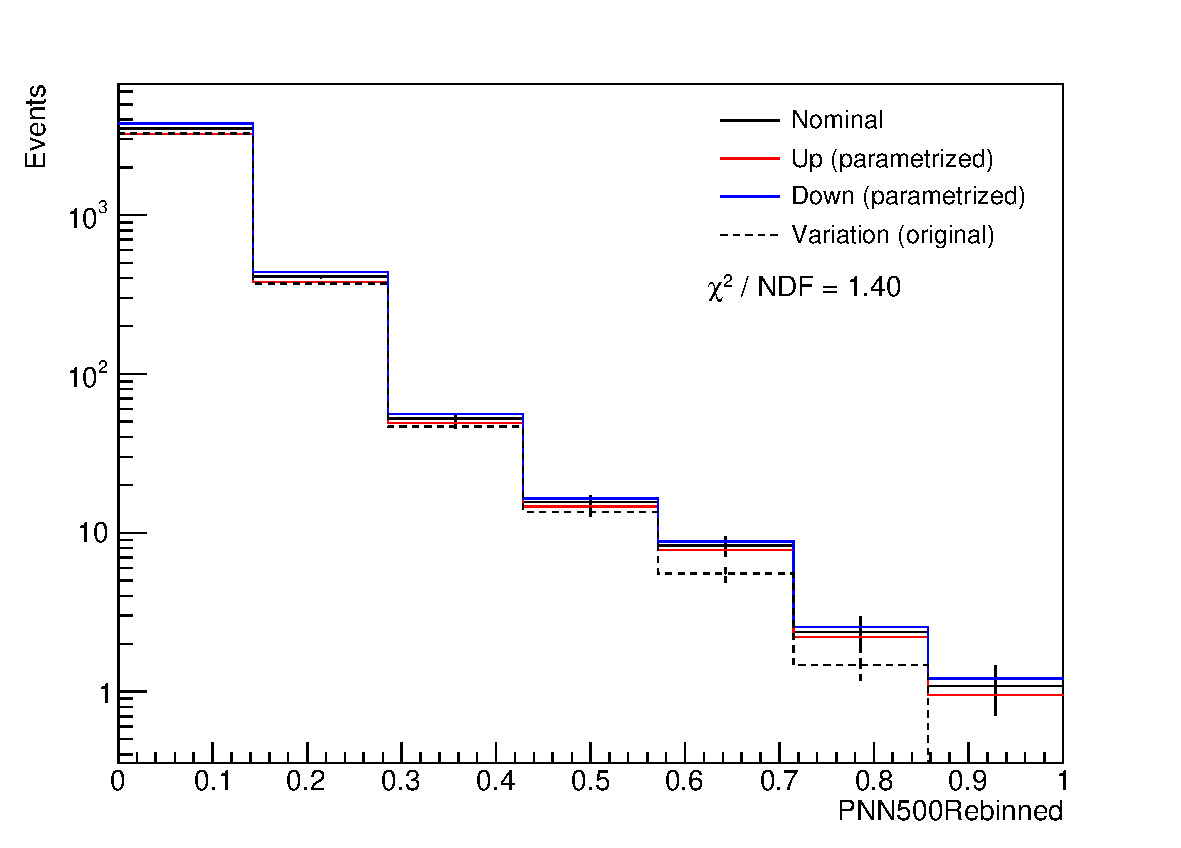
\includegraphics[width=0.32\textwidth]{figures/systs/hadhad_ttbar/ps_pnn500}
% 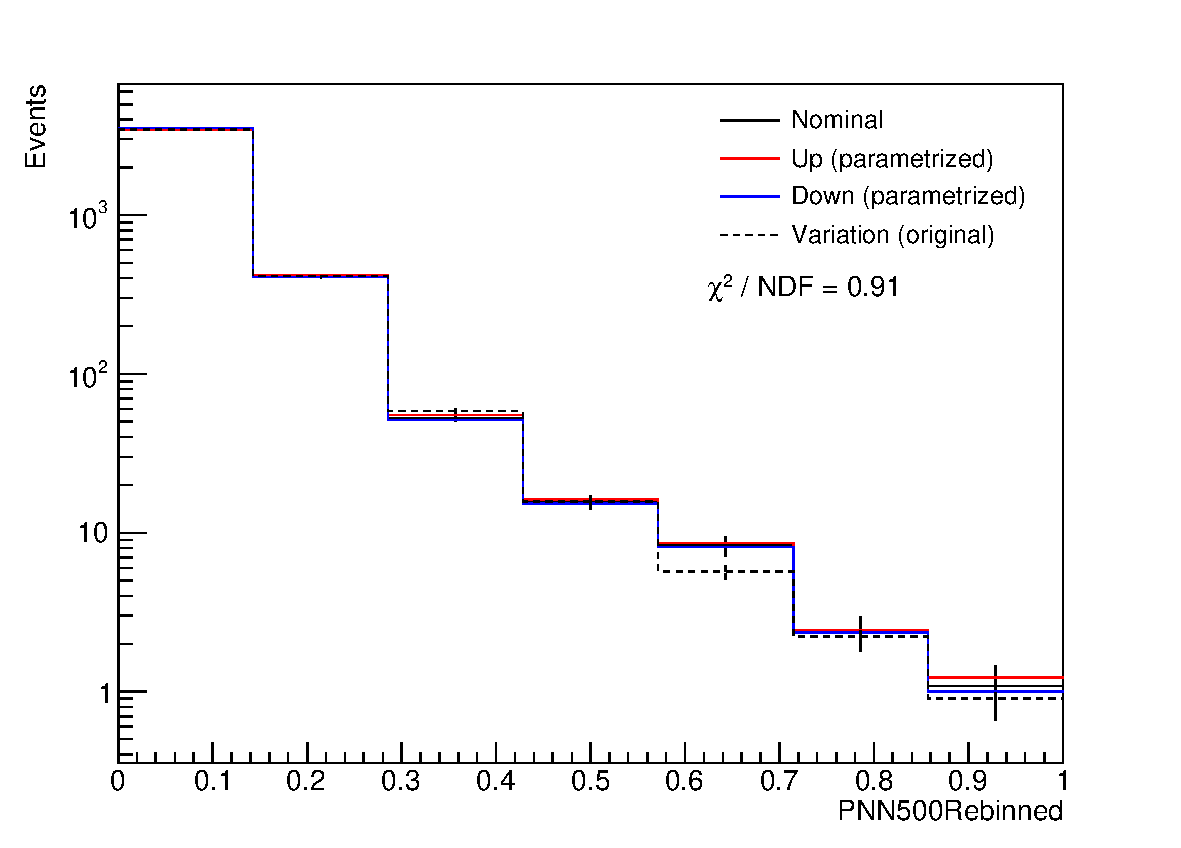
\includegraphics[width=0.32\textwidth]{figures/systs/hadhad_ttbar/isr_pnn500_up}
%   \caption{Closure check of $\tauhad\tauhad$ matrix element (left), parton shower
%     (middle) and ISR uncertainty (right) in the PNN500 distribution used to extract the
%     $X(500) \to b\bar{b}\tauhad\tauhad$ signal.}
%   \label{fig:ttbarsyst_hadhad_closure}
% \end{figure}

% The parametrizations are then passed through the PNN classification, and the resulting variations are shown in Appendix~\ref{subsec:appendix_systs_ttbarsysts_hadhad}.

\paragraph{Uncertainties on $t\bar{t}$ in the Z+HF control region}\mbox{}\\

Shape uncertainties on the $t\bar{t}$ background are neglected in the Z+HF 
control region as they are found to be negligible in the $m_{\ell\ell}$ distribution included in the fit for this region, as shown in Appendix~\ref{subsec:appendix_systs_ttbarsysts_ZCR}.


\subsubsection{Uncertainties on $Z$+HF}
\label{sec:acceptance_uncertainties_ZHF}

The normalisation of the $Z$+hf background is estimated 
from data as included as freely floating parameter in 
the final fit. This normalisation is mainly determined 
from the dedicated $Z$+HF dilepton control region.

Relative acceptance uncertainties are applied on $Z$+hf
in the other regions included in the fit, 
the \hadhad signal region and the \lephad 
signal regions, to take into account potential differences 
in the normalisation between the CR and the SRs.
 
In each signal region also shape variations are checked 
and applied, correlated with the relative acceptance uncertainties on the normalisations, where they are found to be relevant as described in the following. 

All these uncertainties are derived by MC-to-MC comparison, 
as described in Section~\ref{sec:systematics_backgroundmodelling}, 
following the \href{https://twiki.cern.ch/twiki/bin/viewauth/AtlasProtected/PmgWeakBosonProcesses}{\underline{recommendations of the PMG group for Weak Boson processes}}. 


Only Z + heavy flavour jets background are considered, 
including $Z$+bb, $Z$+bc, $Z$+cc. 
Contributions from Z + light flavour jets 
such as $Z$+l, $Z$+bl and $Z$+cl are excluded. 

Uncertainties due to choice of generators are evaluated
by comparing the Sherpa 2.2.1 samples to the
Madgraph+Pythia8 samples. 
Uncertainties on the $Z$+jets background modelling 
related to the choice of renormalisation and factorisation 
scales are evaluated using event weights included 
in the Sherpa 2.2.1 samples, varying the scales either together 
or independently up and down by a factor of two, 
leading to 7-point scale variations. 
The scale uncertainty is then given by the maximum shift 
of the envelope with respect to the nominal, from which 
the envelope around the nominal can be worked out. 
The uncertainty due to the choice of PDF set is evaluated 
in a similar way, using the event weights included in the samples. 
The PDF variations include 100 replicas of the nominal NNPDF3.0 PDF set 
as well as central values for two different PDF set, 
MMHT2014nnlo68cl and CT14nnlo, and two NNPDF3.0nnlo $\alpha_s$ variations.  
The NNPDF intra-PDF uncertainty is estimated as the standard deviation 
of the set of 101 NNPDF3.0 sets. 
The envelope of the differences between the nominal NNPDF set 
and the other two PDF sets is taken as an additional uncertainty. 

From the nominal Sherpa configuration there are two other parameters 
that can be varied to investigate uncertainties 
on the modelling of the $W$/$Z$+jets process: 
Matrix element matching (ckkw), which varies the scale taken 
for the calculation for the overlap between jets 
from the matrix element and the parton shower. 
The nominal value for this parameter is 20 GeV. 
The up variation increases this to 30 GeV, 
while the down variation decreases the nominal value to 15 GeV. 
The second parameter is the resummation scale (qsf), 
which varies the scale used for the resummation 
of soft gluon emission $\mu_{qsf}$ is varied from 2 and with respect to the nominal. 

Relative acceptance normalisation uncertainties between the CR and the SRs are calculated 
from the single channel acceptances using Equation~\ref{eq:relative_acceptance_unc} 
and are found in the different fit regions to be 
as large as reported in Table~\ref{sec:systs:tab:systematics_normalisations_ZHF}.


\begin{table}
\centering
\small
\begin{tabular}{|c|c|c|c|}
\hline
Source & Size in LepHad SLT & Size in LepHad LTT & Size in HadHad\\
\hline
ME & +0.021, -0.021 & +0.10, -0.10 & -0.07, +0.07\\
Scales & -0.029, +0.053 & -0.054, +0.085 & -0.096, +0.12\\
CKKW & +0.07, -0.07 &  +0.071, -0.071 & +0.053, -0.053\\
QSF & -0.016, +0.016 & -0.016 , +0.016 & +0.06, -0.06 \\
PDF+$\alpha_s$ & -0.0026, +0.0026 & -0.0033 , +0.0033 & -0.0077, +0.0077 \\
PDF choice & -0.0097, +0.0097 & -0.011, +0.011 & -0.0098, +0.0098\\
Total & -0.081, +0.092 & -0.14, +0.15 & -0.14, +0.16\\
\hline
\end{tabular}
\caption{Relative size of relative acceptance normalisation uncertainties on $Z$+HF for the di-Higgs analysis.}
\label{sec:systs:tab:systematics_normalisations_ZHF}
\end{table}


\paragraph{Uncertainties on $Z$+HF in the \lephad channel}\mbox{}\\

In the $\tau_{lep}\tau_{had}$ channel the parametrizations of the shape uncertainties 
are derived separately for the SLT channel and the LTT channel. 
Only shape is considered and hence all samples are scaled to one.

The Madgraph samples for comparison are with DSID 361510-361514 for
$m_{ll} > 40$~GeV and 361638-361642 for $10$~GeV $< m_{ll} < 40$~GeV, 
sliced in number of partons. The shape discrepancy between the nominal Sherpa 
samples and the Madgraph samples are propagated through the PNN 
output score. In most of the bins and mass points 
no significant deviation is observed within statistical uncertainty, 
as shown in Appendix~\ref{subsec:appendix_systs_ZHFsysts_lephad}. 
Therefore this uncertainty is ignored for the \lephad channel. 
Furthermore, various kinematic variables are tested to parametrise
the difference in the PNN score where no variables have a significant impact. 


%Uncertainties on the $Z$+jets background modelling related to the choice of renormalisation and factorisation scales are evaluated using event weights included in the Sherpa 2.2.1 samples, varying the scales either together or independently up and down by a factor of two, leading to 7-point scale variations. The scale uncertainty is then given by the maximum shift of the envelope with respect to the nominal, from which the envelope around the nominal can be worked out.
For the scale variations the envelope is characterised 
by the $p_T$ of the two $b$-jets, $p_T^{BB}$, 
as shown in Fig.\ref{fig:lephad_ZHF_scale_pTBB} for the SLT channel the LTT channel. 
Only the shape variation is considered. The discrepancy between 
the nominal sample and the variation sample 
is propagated through the PNN output score, 
the results are shown in Appendix~\ref{subsec:appendix_systs_ZHFsysts_lephad}.

%The uncertainty due to the choice of PDF set is evaluated in a similar way, using the event weights included in the samples. The PDF variations include 100 replicas of the nominal NNPDF3.0 PDF set as well as central values for two different PDF set, MMHT2014nnlo68cl and CT14nnlo, and two NNPDF3.0nnlo $\alpha_s$ variations.  The NNPDF intra-PDF uncertainty is estimated as the standard deviation of the set of 101 NNPDF3.0 sets. The envelope of the differences between the nominal NNPDF set and the other two PDF sets is taken as an additional uncertainty. 

For the PDF variations no obvious shape dependence 
is observed in the PNN score distribution 
comparing the nominal NNPDF set and the standard deviation 
of the 100 replicas. Similarly, no obvious shape dependence 
is found for neither the additional uncertainty CT14nnlo and MMHT2014nnlo68cl 
nor the $\alpha_s$ variations. 
The PNN score distributions of these uncertainties variation 
are shown in Appendix~\ref{subsec:appendix_systs_ZHFsysts_lephad}. 

%From the nominal Sherpa configuration there are another two parameters that can be varied to investigate uncertainties on the modelling of the $W$/$Z$+jets process: Matrix element matching (ckkw), which varies the scale taken for the calculation for the overlap between jets from the matrix element and the parton shower. The nominal value for this parameter is 20GeV. The up variation increases this to 30GeV, whilst the down variation decreases the nominal value to 15GeV. The second parameter is the resummation scale (qsf), which varies the scale used for the resummation of soft gluon emission $\mu_{qsf}$ is varied from 2 and with respect to the nominal. 
The up and down variation for the CKKW and QSF 
uncertainties are both smaller than the nominal sample yields, 
and the solution for this issue is to normalize 
the central value of the up and down variation to the nominal sample, 
and take the difference from there. 
After symmetrizing no shape dependence is observed. 
The PNN score distributions is shown in Appendix~\ref{subsec:appendix_systs_ZHFsysts_lephad}.


\begin{figure}[!h]
\centering
\subfloat[]{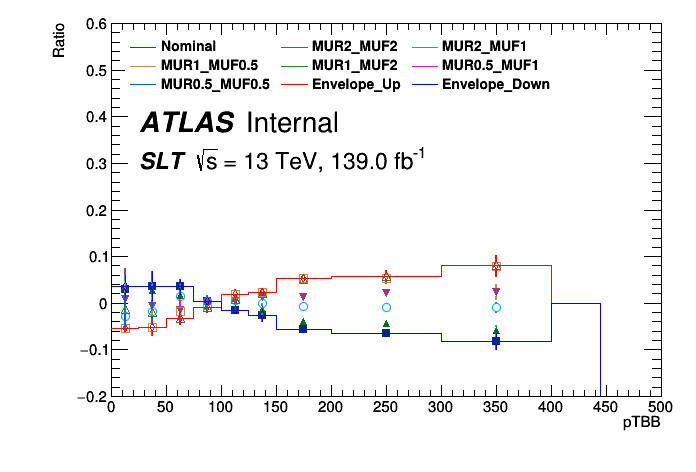
\includegraphics[width=.41\textwidth]{figures/lephad_modelling_systs/SLT/ZHF_scale/Ratio_pTBB_Norm.png}}\quad
\subfloat[]{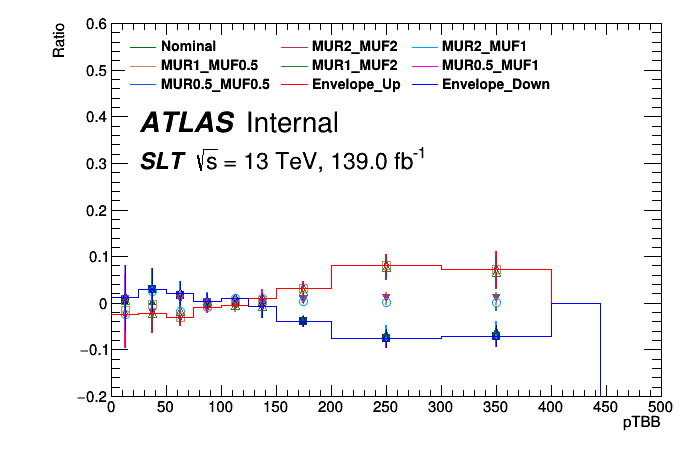
\includegraphics[width=.41\textwidth]{figures/lephad_modelling_systs/LTT/ZHF_scale/Ratio_pTBB_Norm.png}}\quad
\caption{SLT (left) and LTT channel (right): Taking an envelope of the $Z$+HF scale variation with $p_T$ of the 2 $b$-jets.}
\label{fig:lephad_ZHF_scale_pTBB}
\end{figure}


\paragraph{Uncertainties on $Z$+HF in the \hadhad channel}\mbox{}\\

The shape dependence of scales variations are described by the shape of the envelope of 7-point variation, which is directly derived by the maximun (for 1up variation) and minimum (for 1down variation) bin-by-bin on the BDT/PNN score distributions, as shown in Fig.~\ref{fig:hadhad_ZHF_Scale_SMBDT}. Although the \texttt{muR\_muF} may give the largest shape variation for most of the MVA scores, it is shown that the envelope can also estimate the shape dependence reasonably well. Figures for more MVA distributions and detailed studies can be found in Appendix~\ref{subsec:appendix_systs_ZHFsysts_hadhad} and \href{https://indico.cern.ch/event/1042450/contributions/4422123/attachments/2269878/3854717/Z%2Bjets%20modelling%20v3.pdf}{\underline{those slides}}

The comparison with Madgraph samples introduces an shape uncertainty in the $\tau_{had}\tau_{had}$ channel. 
The shape variation can be approximately described by a linear function of the mass of b-jet system ($m_{BB}$), as shown in Fig.~\ref{fig:hadhad_ZHF_Madgraph_mBB}. In $m_{BB}>250$~GeV, the variation is considered to be the same as that at 250 GeV.
Due to the limited statistic of the Madgraph samples, it is still possible that the shape dependence that we observed is originated from fluctuations. 

More details can be found in Appendix~\ref{subsec:appendix_systs_ZHFsysts_hadhad}.

\begin{figure}[htbp]
    \centering
    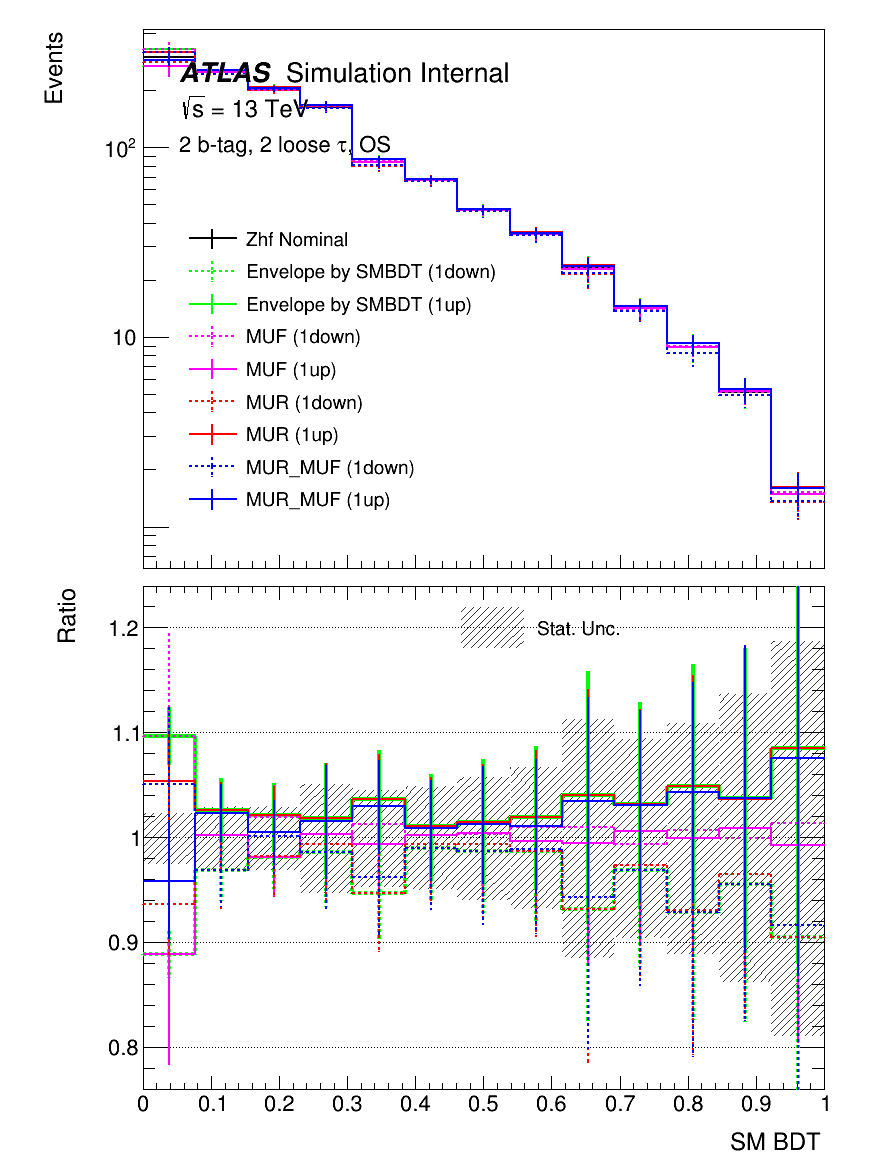
\includegraphics[width=.45\textwidth]{figures/systs/hadhad_ZHF/2tag2pjet_0ptv_LL_OS_SMBDT_BDT_Scale.png}
    \caption{Shape uncertainty of scale ($\mu_R$, $\mu_F$) variations on SMBDT. The black(nominal), pink, red and blue histograms/ratios are the 7-point variations, while the green one is the envelope. Up/down variations are shown in solid/dashed lines. The SMBDT score is transformed into the binning of the final fit. The shaded area shows the statistical uncertainty of the nominal samples.}
    \label{fig:hadhad_ZHF_Scale_SMBDT}
\end{figure}

\begin{figure}[htbp]
    \centering
    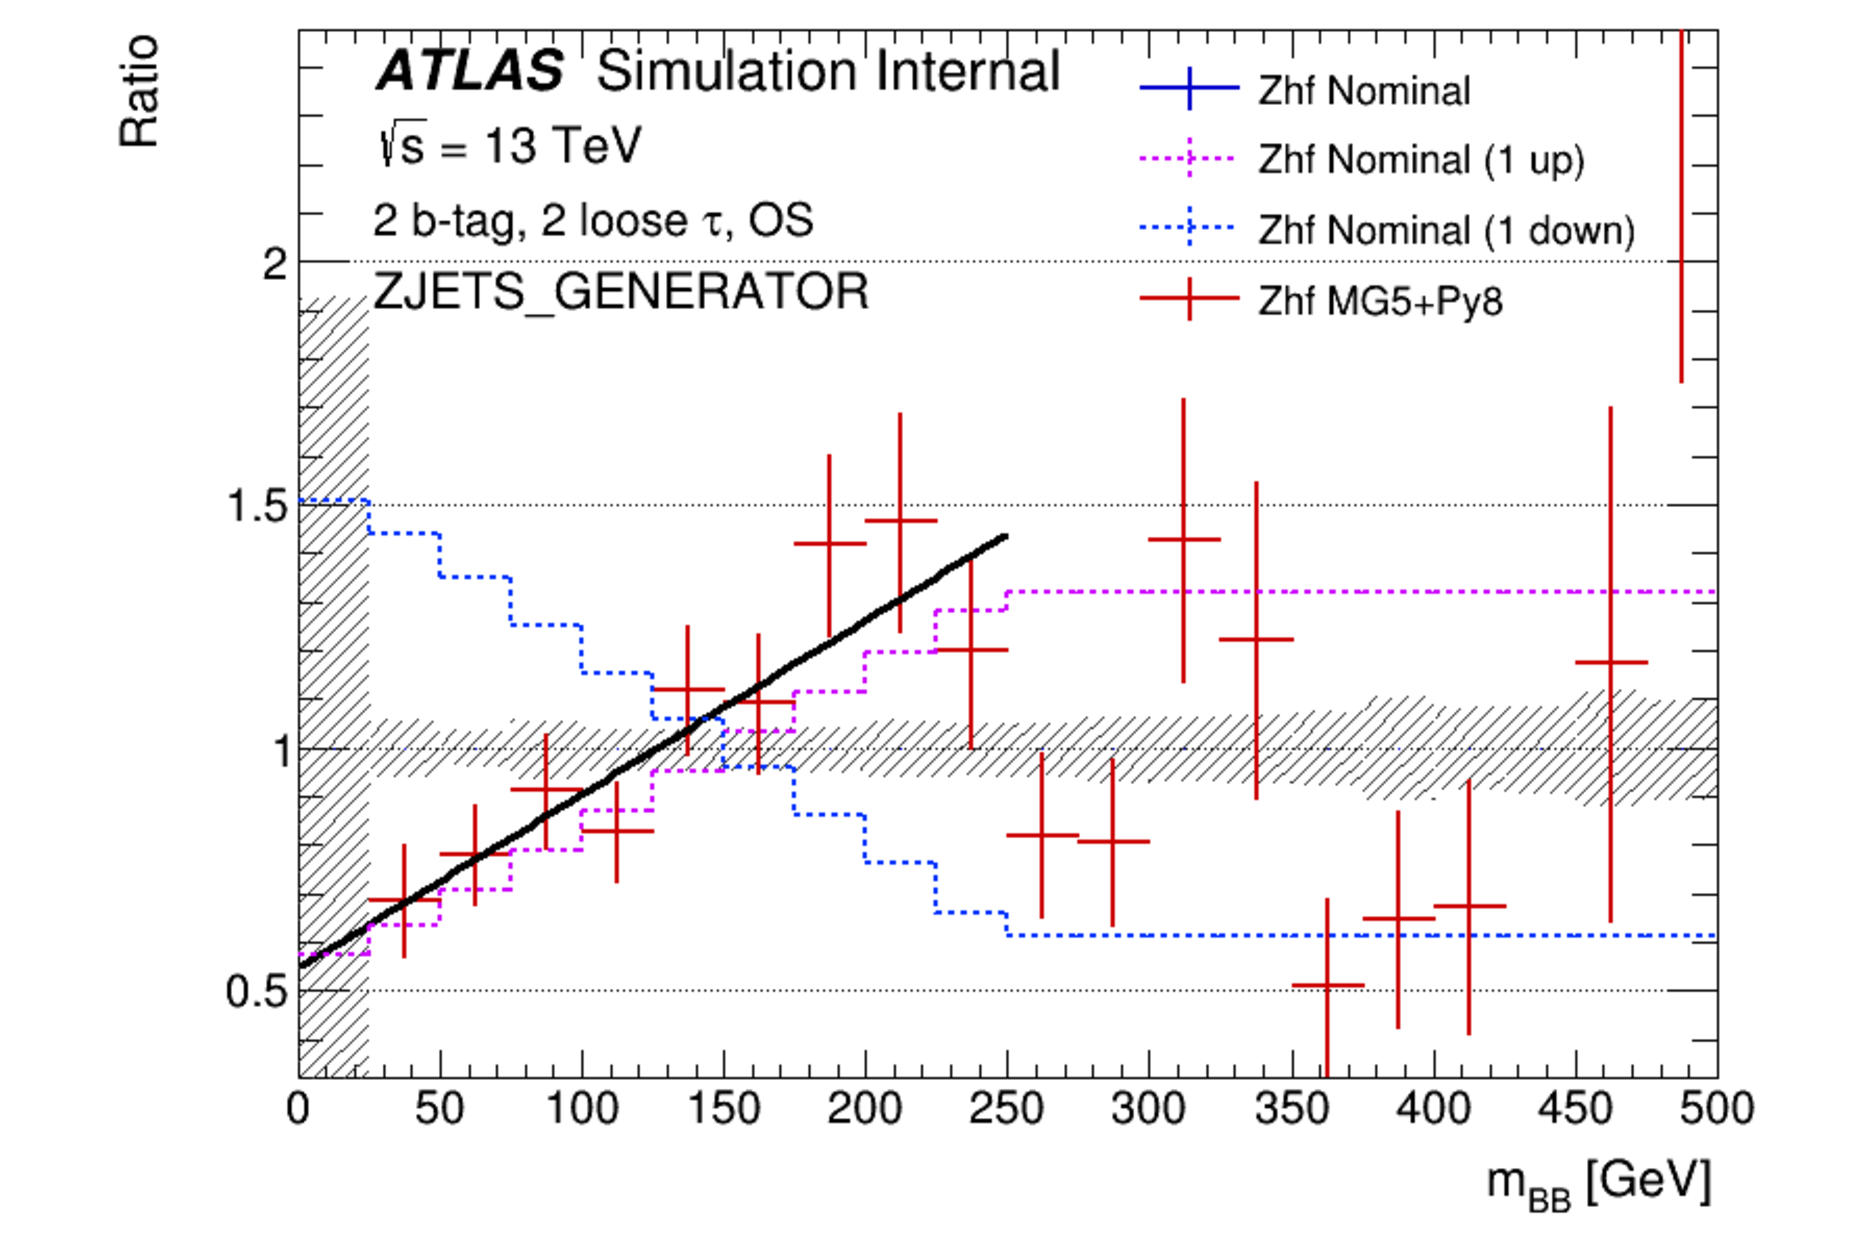
\includegraphics[width=.45\textwidth]{figures/systs/hadhad_ZHF/2tag2pjet_0ptv_LL_OS_mBB_Presel}
    \caption{Madgraph comparison uncertainty of Z+HF in the HH $\tau_{had}\tau_{had}$ signal region. The "Nominal" samples are generated by Sherpa, "MG5+Py8" represents the Madgraph samples. The black line in the ratio plot is the parametrisation derived with the $m_{BB}$ distribution, which corresponds to the "up" variation~($0.55 + 0.0035 \times m_{BB}~\text{if}~m_{BB}\le 250~\GeV;~1.43~\text{if}~m_{BB} > 250~\GeV$). The down variation is the symmetric mirror of the up variation. The dotted lines are the final up and down variations estimated by the parametrised uncertainty. The shaded area shows the statistical uncertainty of the nominal samples.}
    \label{fig:hadhad_ZHF_Madgraph_mBB}
\end{figure}

Other shape uncertainties on the $Z$+HF background are neglected in the \hadhad signal region as they are found to be negligible, as shown in Appendix~\ref{subsec:appendix_systs_ZHFsysts_hadhad}.


\paragraph{Uncertainties on $Z$+HF background in the Z+HF control region}\mbox{}\\

Shape uncertainties on the $Z$+HF background are neglected in the Z+HF control region as they are found to be negligible in the $m_{ll}$ distribution included in the fit for this region, as shown in Appendix~\ref{subsec:appendix_systs_ZHFsysts_ZCR}.



\subsubsection{Uncertainties on single top}
\label{sec:uncertainties_singletop}

All single-top uncertainties are derived by MC-to-MC comparison,  and split into the normalisation acceptance uncertainties and the 
shape uncertainties,  as described in Section~\ref{sec:systematics_backgroundmodelling}, 
following the  \href{https://twiki.cern.ch/twiki/bin/view/AtlasProtected/TopMCSystematicsR21}{\underline{recommendations of the Top modelling group}}. 

Uncertainties due to PDF, additional radiation (ISR) and FSR are evaluated using internal alternative weights present in all single-top nominal samples. 
Using the \texttt{PDF4LHC15\_30} PDF set, the uncertainties are estimated by combining the difference between the error sets and the nominal set following the recommendations in Ref.\cite{Butterworth:2015oua}.

Uncertainties from the parton shower, matrix element (ME) and single top interference ($Wt$-channel) are estimated using 
the differences between the nominal samples and the corresponding alternative samples, as reported in Table~\ref{sec:systs:tab:systematics_singletop}. 
As the $W$t-channel contribution dominates over the $t$-channel and $s$-channel contributions, only the contribution from the $Wt$-channel 
is considered. Parton shower and hadronisation uncertainties (PS) are evaluated comparing the AF2 nominal samples showered with Pythia8 
with alternative AF2 samples showered with Herwig7.  The ME NLO matching uncertainty is evaluated comparing  the AF2 nominal Powheg+Pythia8 
samples to the alternative AF2 aMcAtNlo+Pythia8 samples.  Uncertainty due single-top interference is evaluated comparing the full simulated nominal 
Powheg+Pythia8 samples with diagram removal (DR) scheme to the alternative full simulation Powheg+Pythia8 sample with diagram subtraction (DS) 
scheme.

\begin{table}
  \centering
  \begin{tabular}{|c|c|c|}
  \hline
  Source & DSID & Name\\
  \hline
  Nominal & 410646, 410647 &PowhegPythia8EvtGen\_A14\_Wt\_DR\_inclusive \\
  ME & 412002 &aMcAtNloPythia8EvtGen\_HThalfscale\_tW\_inclusive\\
  PS & 411036,411037   &PowhegHerwig7EvtGen\_H7UE\_Wt\_DR\_inclusive \\
  single top interference &410654,410655 &PowhegPythia8EvtGen\_A14\_Wt\_DS\_inclusive \\
   
  \hline
  \end{tabular}
  \caption{List of nominal and alternative single-top samples for PS, ME, single top interference uncertainties.}
  \label{sec:systs:tab:systematics_singletop}
  \end{table}
  

To evaluate the shape uncertainties, differences between the AF2 alternative samples and the AF2 nominal sample 
are parametrised by kinematic variables' distributions, and the parametrisation is applied on the full simulated nominal 
sample as weights. The weighted nominal sample is then run through the same pre-selection and the same PNN 
classification. The distributions of other kinematic variables, which are not used for the parametrisation and the PNN scores 
are checked for different choices of the parametrisation variables.  Various kinematic variables are considered for the 
parametrisation. Finally, the variable to parametrise is chosen such that the weighted nominal sample can best recover 
the PNN scores of the systematics variations. 

\paragraph{Uncertainties on single-top background in the \lephad channel}\mbox{}\\

The normalisation acceptance uncertainties are shown in Table~\ref{sec:systs:tab:systematics_normalisations_singletop}.

\begin{table}
\centering
\small
\begin{tabular}{|c|c|c|c|}
\hline
Source & Size in LepHad SLT & Size in LepHad LTT & Size in HadHad \\
\hline
ME & -0.022, +0.022 & -0.15, +0.15 & +0.049, -0.049 \\  
PS & +0.077, -0.077 & -0.093, +0.093 & -0.16, +0.16 \\
Single top interference & +0.078, -0.078 & +0.11, -0.11 & +0.27,-0.27 \\
ISR & -0.047, +0.064 & -0.045, +0.062 & -0.049, +0.066 \\ 
FSR & -0.054, +0.043 & -0.069, +0.035, & -0.094, +0.087\\
PDF & -0.032, +0.032 & -0.032, +0.032 &  -0.032, +0.032 \\
Total & $\pm 13.7\%$ & $\pm 21.1\%$ & $\pm 33.7\%$  \\
\hline
\end{tabular}
\caption{Relative size of normalisation acceptance uncertainties for single-top background for the $HH$  analysis.}
\label{sec:systs:tab:systematics_normalisations_singletop}
\end{table}

%\begin{table}
%\centering
%\small
%\begin{tabular}{|c|c|c|c|}
%\hline
%Source & Size in LepHad SLT & Size in LepHad LTT & Size in HadHad \\
%\hline
%ME & $\pm2.2\%  $ & $\pm15.3\%  $ & $\pm 4.9\%$ \\  
%PS & $\pm7.7\% $ & $\pm9.3\% $ & $\pm 16\%$ \\
%Single top interference & $\pm7.8\%$ & $\pm11.4\%  $ & $\pm 27\%$ \\
%ISR &$+6.4\%,-4.7\%$ & $+6.2\%,-4.5\%$ & $+6.6\%, -4.9\%$ \\ 
%FSR &$+4.3\%,-5.4\%$ & $+3.5\%,-6.9\%$ & $+8.7\%, -9.4\%$\\
%PDF & $\pm 3.2\%$ & $\pm 3.2\%$ &  $\pm 3.2\%$ \\
%Total & $\pm 13.7\%$ & $\pm 21.1\%$ & $\pm 33.7\%$  \\

%Scale:muR & $+5.5\%,-5.2\%$  &$+5.9\%,-5.5\%$ \\
%Scale:muF & $+2.1\%,-2.0\%$  &$+1.9\%,-1.8\%$ \\
%ISRalphas & $+2.1\%,-1.8\%$  &$+1.2\%,-1.3\%$ \\
%\hline
%\end{tabular}
%\caption{Relative size of normalisation acceptance uncertainties for single-top background for the $HH$  analysis.}
%\label{sec:systs:tab:systematics_normalisations_singletop}
%\end{table}



  
The shape uncertainty is derived separately for the SLT channel and the LTT channels. The variations are parametrised by the 
ratio of the alternative sample to the nominal sample in bins of kinematic variables. 

Only normalisation acceptance uncertainty is considered for the ME and PS uncertainties as no obvious shape is observed in 
the NN (classification used for SM signal) or the PNN score. The NN score distributions are shown in Fig.\ref{fig:singletopsyst_lephad_aMC_NN} for the aMC systematic
and in Fig.\ref{fig:singletopsyst_lephad_herwig_NN} for the Herwig systematic.
The PNN score distributions are shown in Appendix~\ref{subsec:appendix_systs_singletop}. 
The FSR, scale, ISR and $\alpha_s$ uncertainties are 
implemented by the internal weights of the single top MC samples therefore no parametrisation is needed. 

For the single-top interference uncertainty, the parametrisation is extracted from the ratio of the variation to the nominal fullsim samples
in bins of \pt\ of two b-jets ($p_T^{bb}$). The parametrisation is applied on the nominal sample and passed through the PNN 
classification used for signal extraction for validation. Finally the weighted nominal PNN score distribution is then compared with the PNN 
score of the variation. The parametrisation is shown in 
Fig.\ref{fig:singletopsyst_lephad_interference_pTBB} (a), (b) for the SLT and the LTT channels respectively.

The closure in the NN score (the classification used for SM signal) for the 
systematics and the weighted nominal are shown in 
Fig.\ref{fig:singletopsyst_lephad_interference_NN}. 
The PNN score of the weighted nominal sample along with the interference uncertainty is shown in Appendix~\ref{subsec:appendix_systs_singletop}, 
in which the shape is covered well by the reweighted nominal distribution. 


\begin{figure}
  \centering
  \subfloat[]{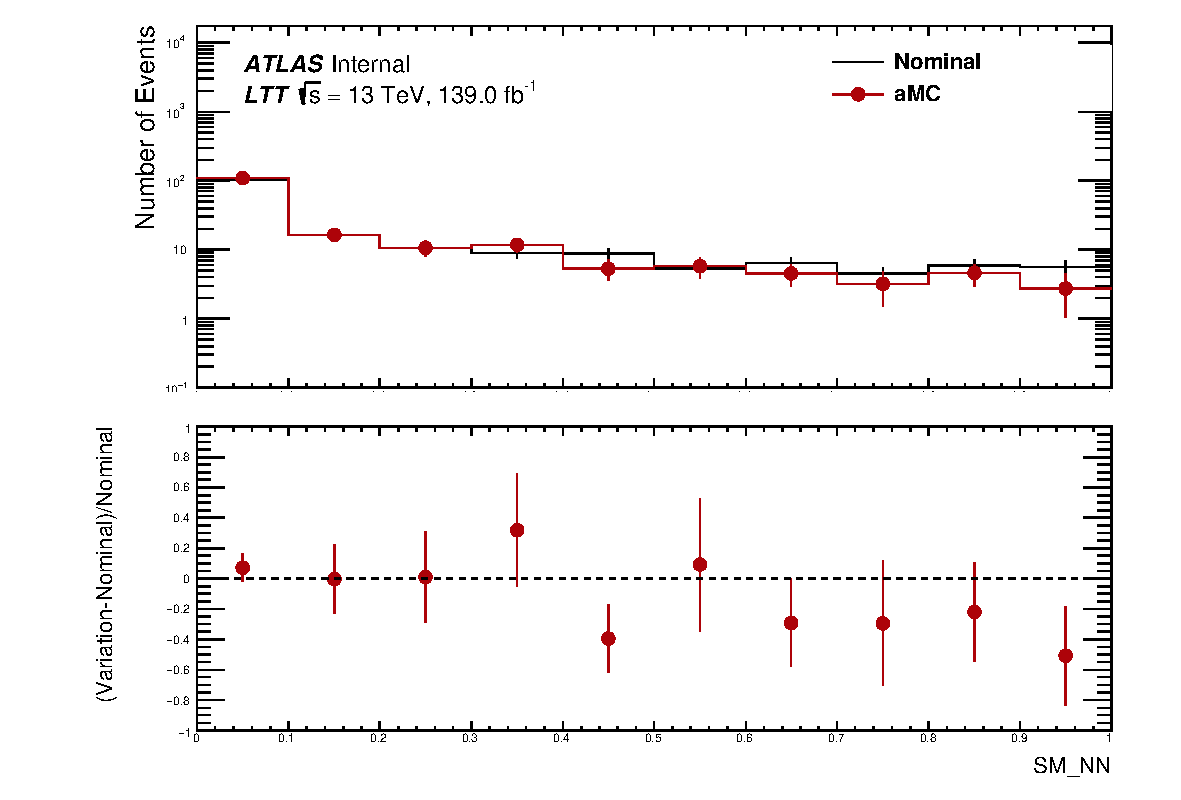
\includegraphics[width=.49\textwidth]{figures/lephad_modelling_systs/LTT/singletop/aMC/Hist_and_ratio_SM_NN_Norm}}
  \subfloat[]{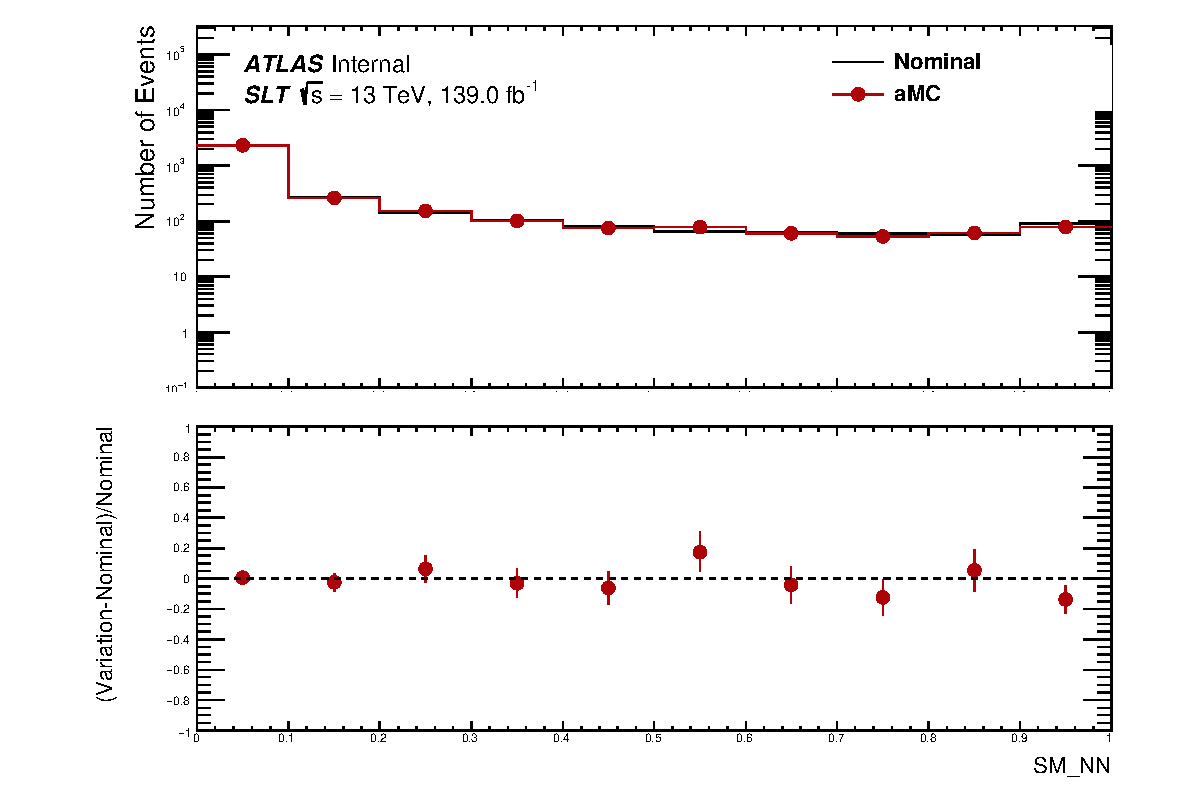
\includegraphics[width=.49\textwidth]{figures/lephad_modelling_systs/SLT/singletop/aMC/Hist_and_ratio_SM_NN_Norm}}
  \caption{LTT (left) and SLT channels (right): shape only SM NN score of the aMC uncertainty .}
  \label{fig:singletopsyst_lephad_aMC_NN}
  \end{figure}


  \begin{figure}
    \centering
    \subfloat[]{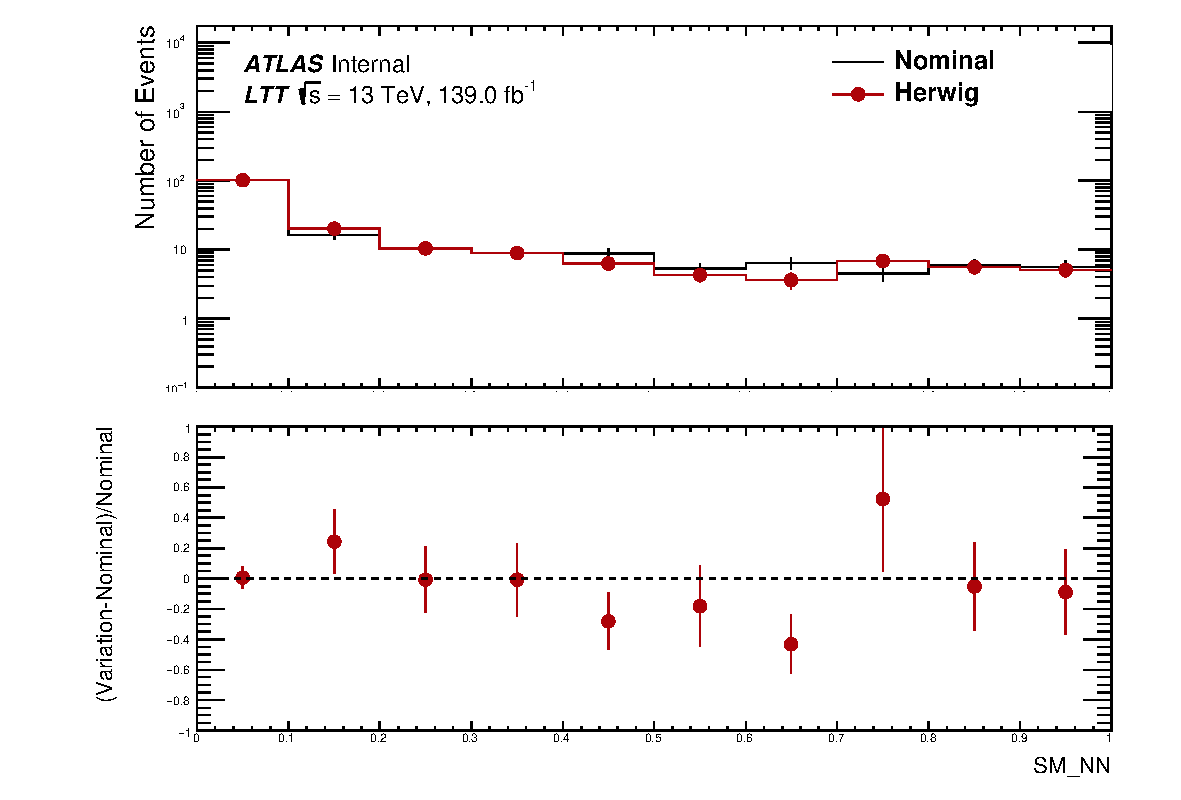
\includegraphics[width=.49\textwidth]{figures/lephad_modelling_systs/LTT/singletop/Herwig/Hist_and_ratio_SM_NN_Norm}}
    \subfloat[]{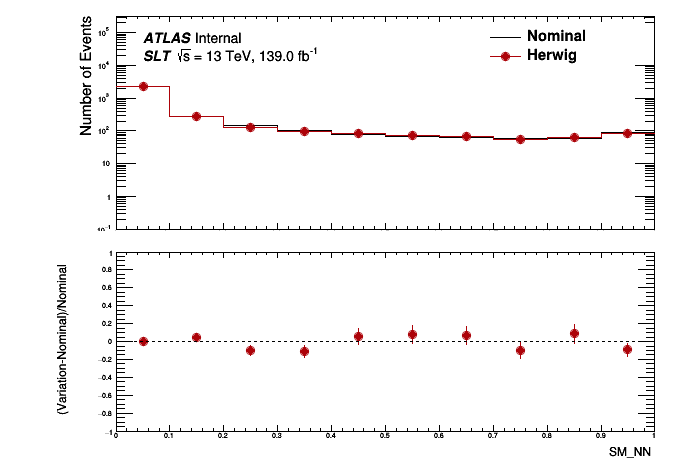
\includegraphics[width=.49\textwidth]{figures/lephad_modelling_systs/SLT/singletop/Herwig/Hist_and_ratio_SM_NN_Norm}}
    \caption{LTT (left) and SLT channels (right): shape only SM NN score of the Herwig uncertainty .}
    \label{fig:singletopsyst_lephad_herwig_NN}
    \end{figure}


\begin{figure}
\centering
\subfloat[]{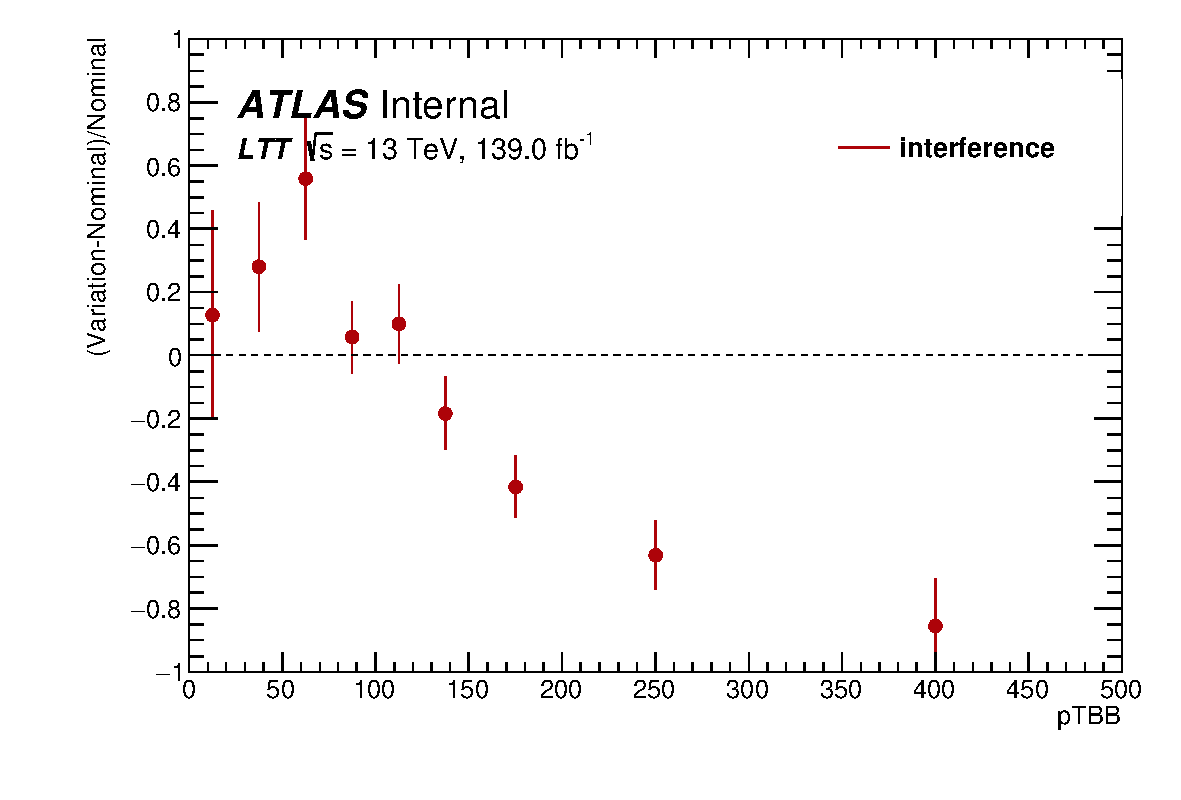
\includegraphics[width=.49\textwidth]{figures/lephad_modelling_systs/LTT/singletop/interference/pTBB_Norm}}
\subfloat[]{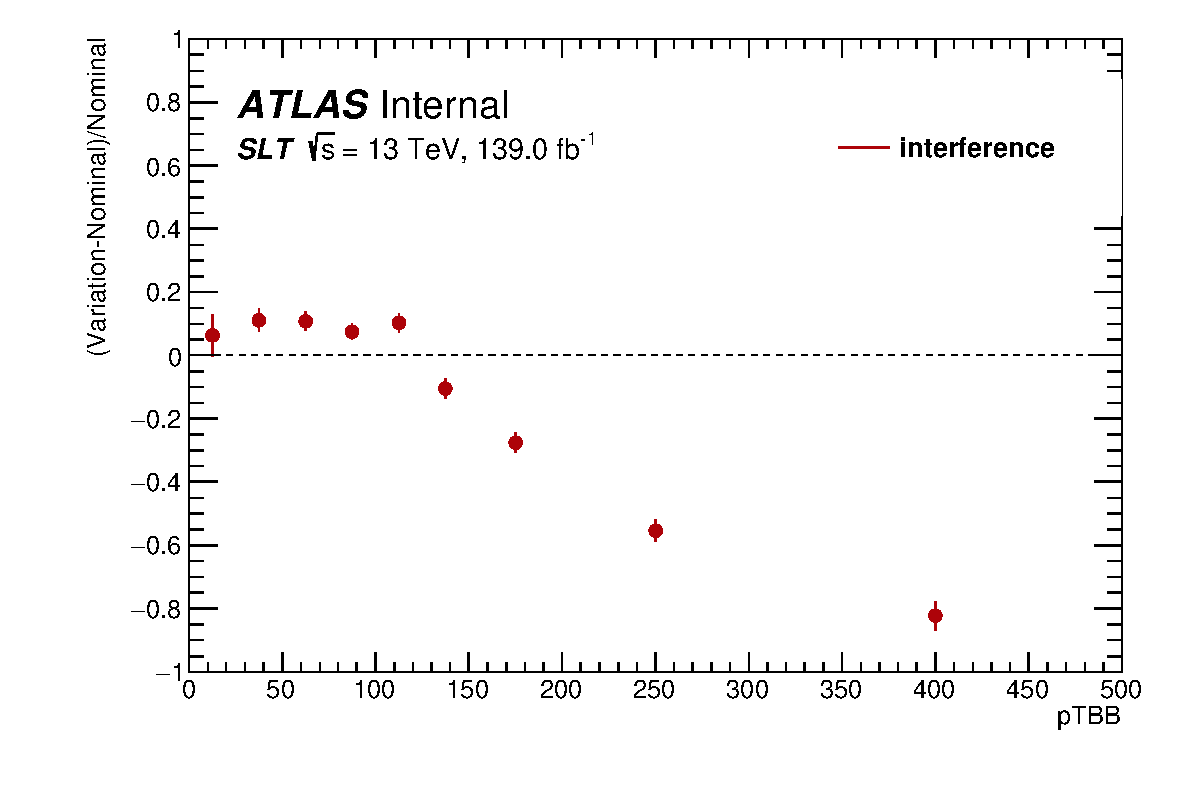
\includegraphics[width=.49\textwidth]{figures/lephad_modelling_systs/SLT/singletop/interference/pTBB_Norm}}
\caption{LTT (left) and SLT channels (right): shape only Parametrisation in bins of $p_T^{bb}$ distribution for $Wt$ DS/DR interference uncertainty.}
\label{fig:singletopsyst_lephad_interference_pTBB}
\end{figure}

\begin{figure}
  \centering
  \subfloat[]{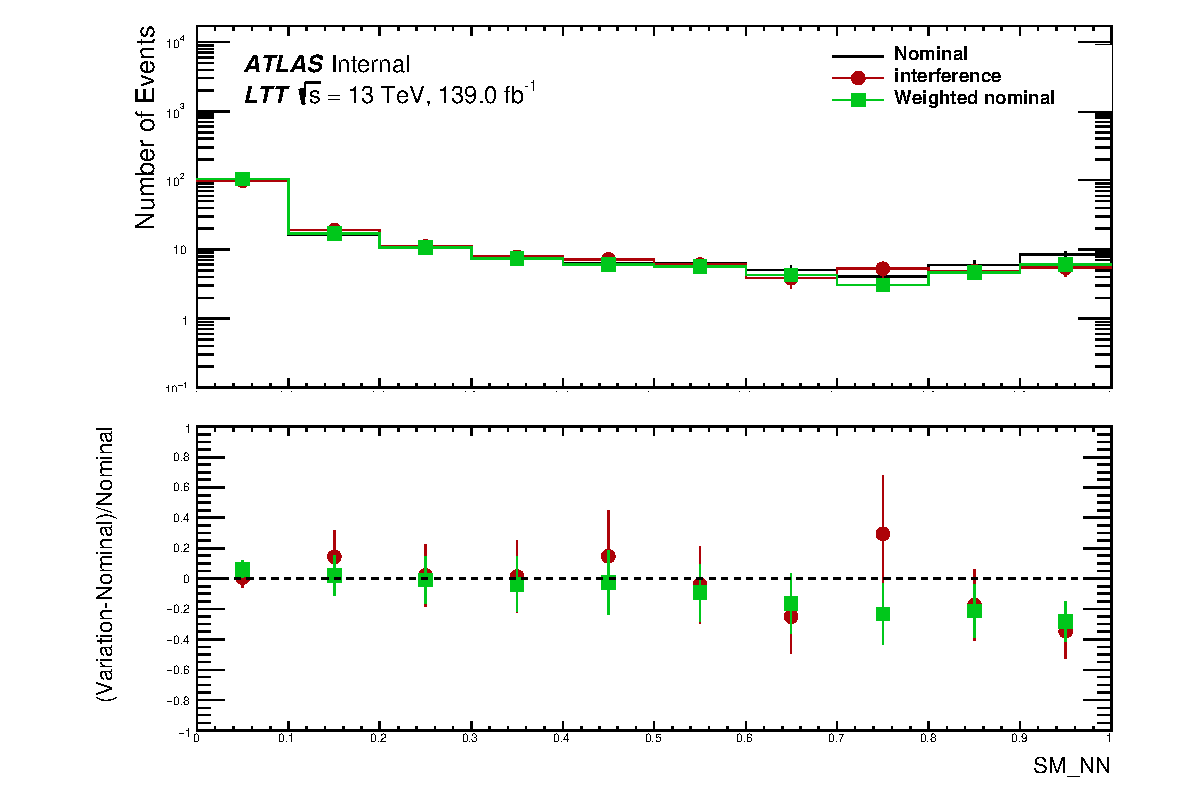
\includegraphics[width=.49\textwidth]{figures/lephad_modelling_systs/LTT/singletop/interference/Hist_and_ratio_SM_NN_Norm}}
  \subfloat[]{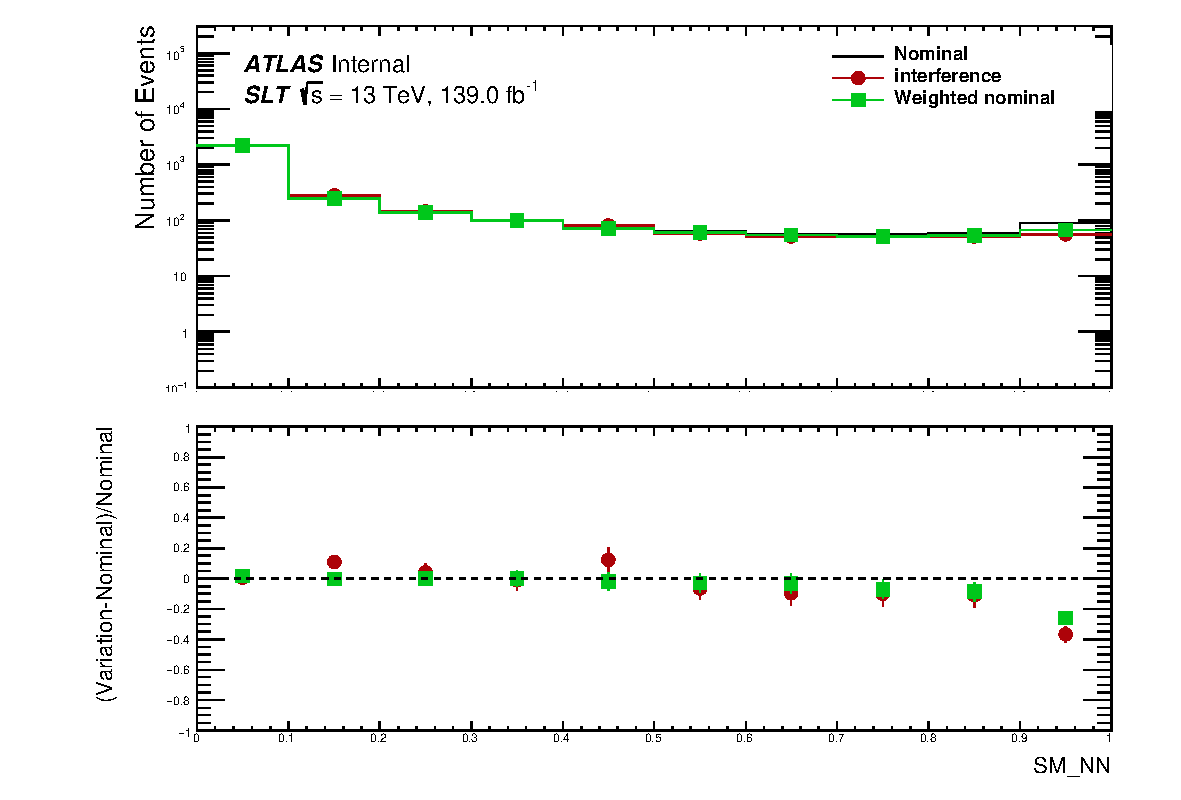
\includegraphics[width=.49\textwidth]{figures/lephad_modelling_systs/SLT/singletop/interference/Hist_and_ratio_SM_NN_Norm}}
  \caption{LTT (left) and SLT channels (right): shape only SM NN score of the $Wt$ DS/DR interference uncertainty .}
  \label{fig:singletopsyst_lephad_interference_NN}
  \end{figure}


\paragraph{Uncertainties on single-top background in the \hadhad channel}\mbox{}\\

The contribution in single-top is even smaller in the \hadhad channel. 
The uncertainties are derived the same way as \lephad channel.
For the uncertainties related to ME, PS, ISR, FSR and PDF variations, only normalisation effect is considered, as summarised in Table~\ref{sec:systs:tab:systematics_normalisations_singletop}. 
For the top interference uncertainty, similar as \lephad channel, the variation (shape+norm.) is parametrised in bins of $p_T^{bb}$, as shown in the ratio plot of Fig.~\ref{fig:singletopsyst_hadhad_interference_pTBB}. Closure of the parametrisation is checked in various BDT/PNN distributions. Good performance is achieved, which can be seem from~\ref{fig:singletopsyst_hadhad_interference_MVA}.
More details about the impact of each variation on the BDT/PNN score distribution can be found in \ref{subsec:appendix_systs_singletop}.

\begin{figure}
  \centering
  \caption{Parametrisation in bins of $p_T^{bb}$ distribution for top interference uncertainty on single-top Wt-channel for \hadhad.}
  \label{fig:singletopsyst_hadhad_interference_pTBB}
\end{figure}

\begin{figure}
  \centering
  \subfloat[]{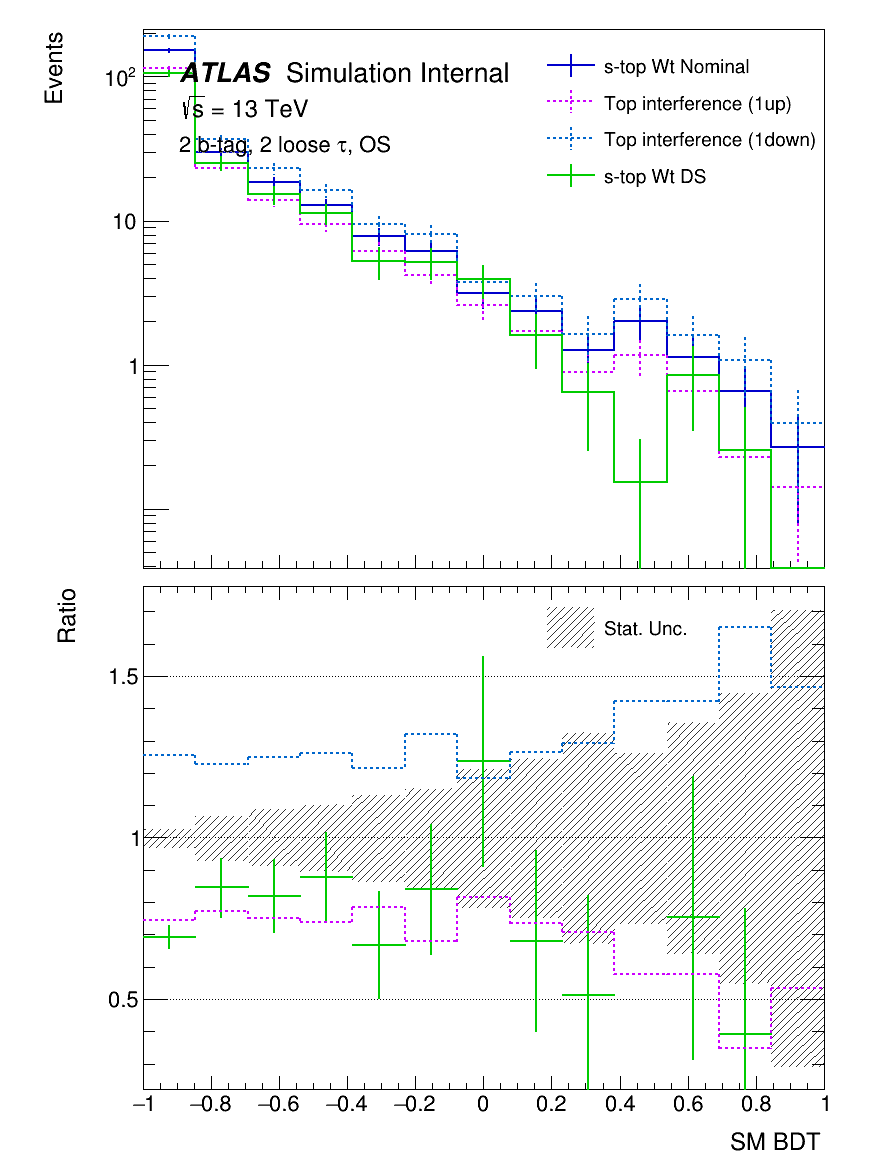
\includegraphics[width=.245\textwidth]{figures/systs/hadhad_stop/2tag2pjet_0ptv_LL_OS_SMBDT_Wt_DS_BDT}}
  \subfloat[]{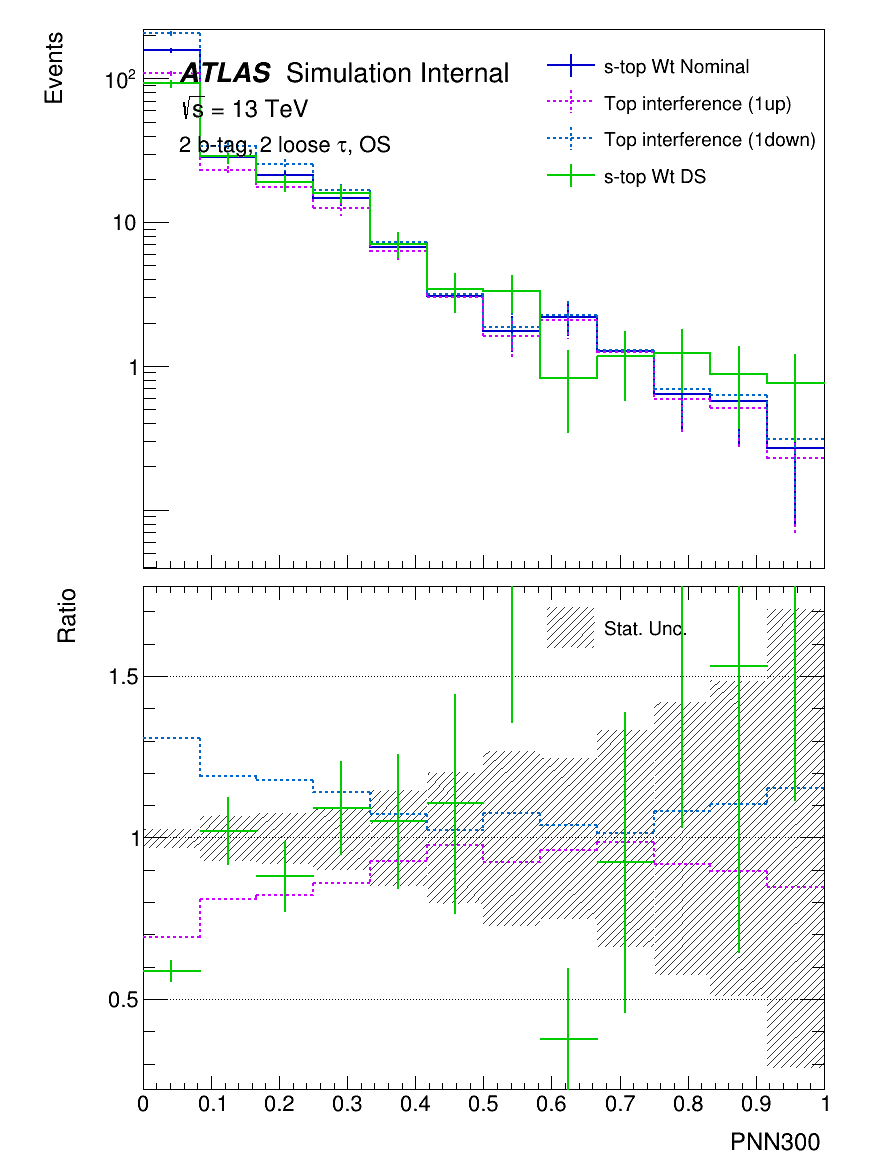
\includegraphics[width=.245\textwidth]{figures/systs/hadhad_stop/2tag2pjet_0ptv_LL_OS_PNN300_Wt_DS_PNN}}
  \subfloat[]{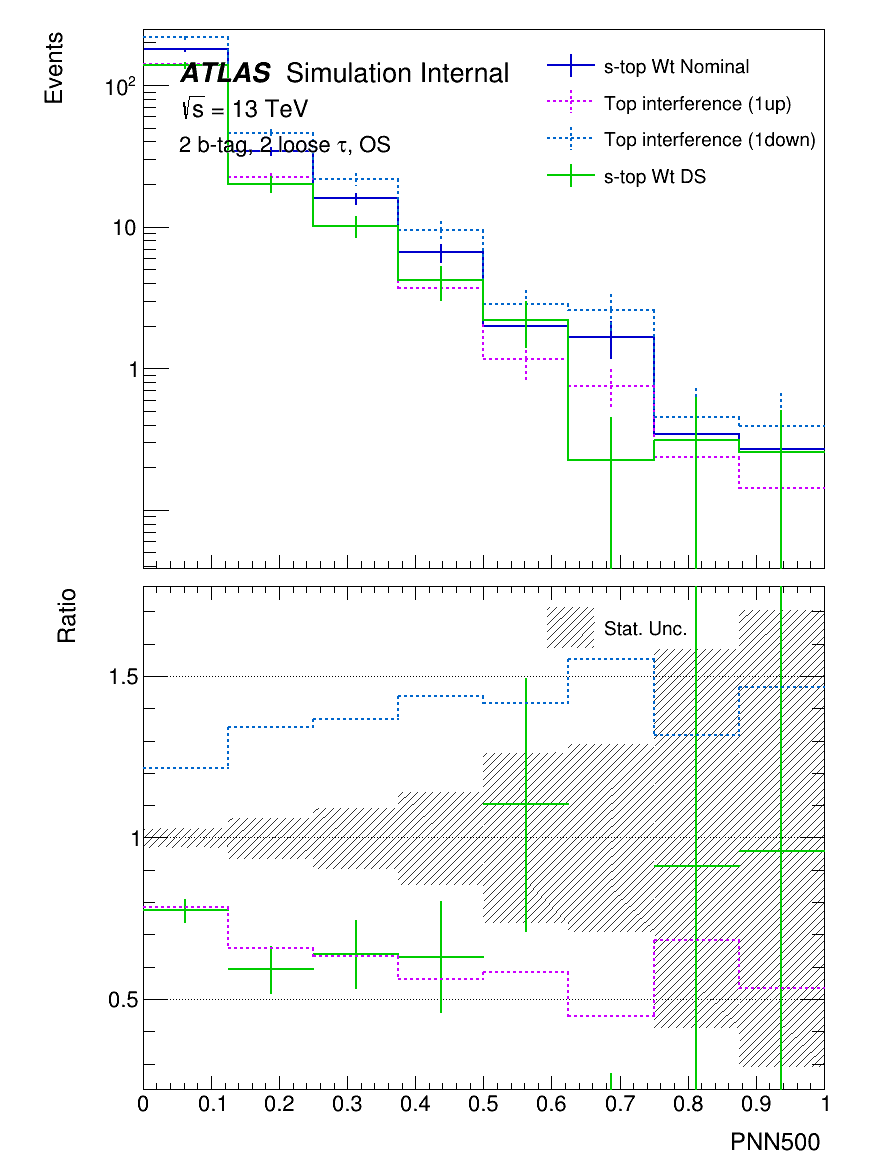
\includegraphics[width=.245\textwidth]{figures/systs/hadhad_stop/2tag2pjet_0ptv_LL_OS_PNN500_Wt_DS_PNN}}
  \subfloat[]{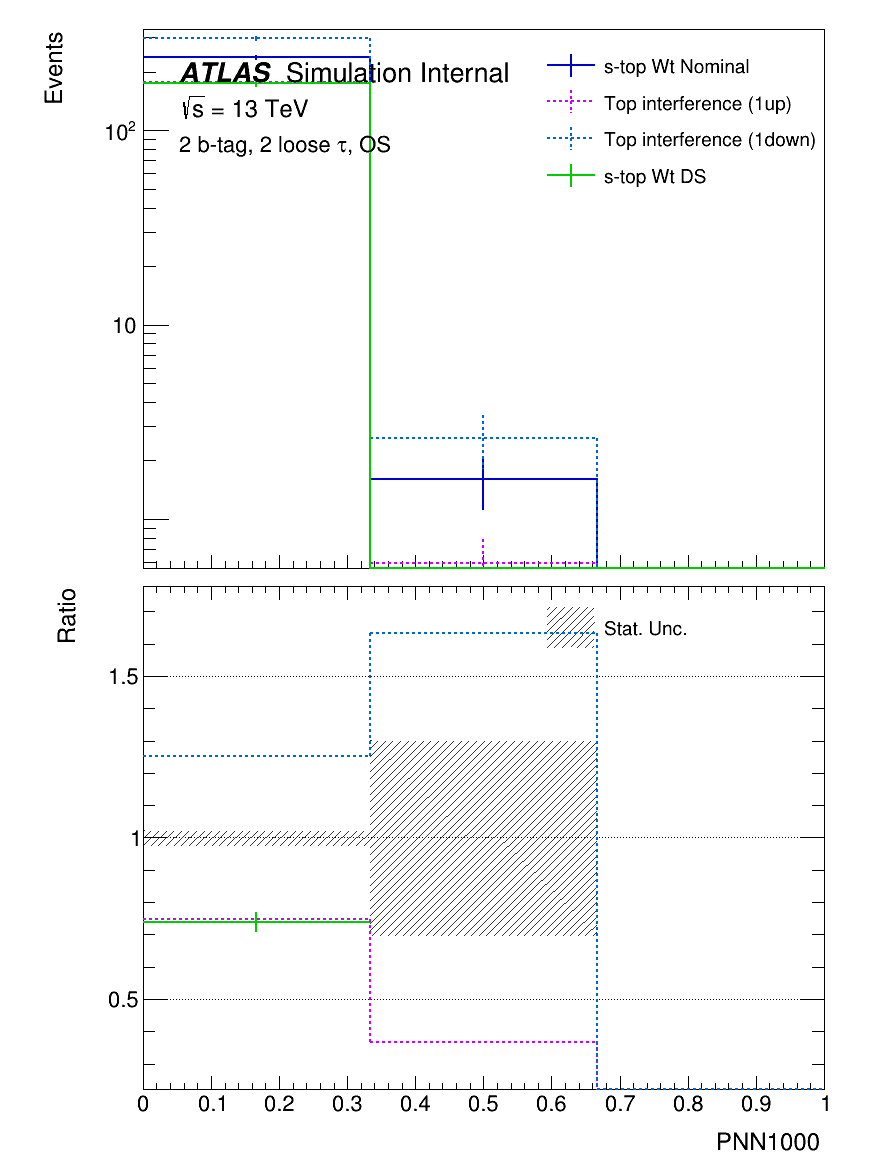
\includegraphics[width=.245\textwidth]{figures/systs/hadhad_stop/2tag2pjet_0ptv_LL_OS_PNN1000_Wt_DS_PNN}}
  \caption{Top interference uncertainty on single-top Wt-channel for \hadhad, in different BDT and PNN distributions.}
  \label{fig:singletopsyst_hadhad_interference_MVA}
\end{figure}

%\begin{table}
%  \centering
%  \small
%  \begin{tabular}{|c|c|}
%  \hline
%  Source & Size in HadHad SR \\
%  \hline
%  ME & $\pm 4.9\%$  \\
%  PS & $\pm 16\%$  \\
%  Single top interference & $\pm 27\%$ \\
%  ISR & $+6.6\%, -4.9\%$ \\
%  FSR & $+8.7\%, -9.4\%$ \\
%  PDF & $+3.2\%, -3.2\%$ \\
%  Total & $\pm 33\%$  \\
%  \hline
%  \end{tabular}
%  \caption{Normalisation acceptance uncertainties for single-top background for the $HH$ \hadhad analysis.}
%  \label{sec:systs:tab:systematics_normalisations_singletop_hadhad}
%\end{table}
  


% \subsubsection{Uncertainties on single-Higgs}
% \label{subsec:uncertainties_singleHiggs}

% Cross section and BR uncertainties are applied to all single-Higgs processes included in the analysis as backgrounds (following recommendations from LHC Higgs Working Group). In addition to those, a 100\% uncertainty is applied on the normalisation of the single-Higgs processes without real $b$-quarks (ggFHtautau, VBFHtautau and WHtautau) to account for modelling of Higgs processes in association with extra heavy flavor (conservative uncertainty motivated by studies of heavy-flavour production in association with top-quark pairs~\cite{PhysRevD.89.072012} and W boson production in association with b-jets~\cite{Aad_2013} and from more recent ttHyy studies~\cite{MorenoLlacer:2684286}, applied in all di-Higgs analyses where relevant). No heavy-flavour uncertainty is assigned to the ttH and ZH production modes, where the dominant heavy-flavour contribution is already accounted for in the LO process.

Acceptance uncertainties on ttH and ZH are evaluated in the phase-space of the signal regions of this analysis by MC-to-MC comparison.

Uncertainties due to PDF, $\alpha_s$ and scales are evaluated using internal alternative weights present in all the single-Higgs nominal samples. 

For PDF and $\alpha_s$ variations, the PDF4LHC\_ NLO\_ 30 uncertainty sets, consisting of 30 eigenvectors parameterising the uncertainties for all the PDFs and 1 parameter for the $\alpha_s$ variations, are used and are compared to the nominal PDF4LHC\_ NLO \_ 30 to evaluate the size of the variations (as recommended by the Higgs group even if the nominal PDF used in the nominal sample is the NNPDF30NNLO PDF set). These variations are combined following the PDF4LHC recommendations~\cite{Butterworth:2015oua}, consisting in evaluating the PDF uncertainty $\delta_{PDF}$ by calculating the square root of the sum in quadrature of the 30 variations, evaluating the $\alpha_s$ uncertainty by taking the half difference between the same PDF set with two different $\alpha_s$ values, and then adding in quadrature the two contributions of $\delta_{PDF}$ and $\alpha_s$ uncertainties to obtain the total uncertainty, in each bin of the PNN score distribution.

Variations of the renormalisation and factorisation scales are used to estimate the uncertainty due to missing higher order corrections. For these scale variations, the 7-point scale variations of the renormalisation ($\mu_R$) and the factorisation scale ($\mu_F$) are used and they are combined by taking an envelope of all of the variations (as recommended by the Physics Modelling group), in each bin of the PNN score distribution.

Parton shower hadronisation algorithmic uncertainties are evaluated comparing samples showered with Pythia and Herwig (with the ME provided by the same generator) to have an handle on the differences between the PS and non-perturbative models as Pythia and Herwig use different algorithms for the parton shower and for the non-perturbative modeling (hadronisation, MPI). The list of single-Higgs alternative samples used for PS uncertainties is given in Table~\ref{sec:systs:tab:systematics_singleHiggssamples_PS}.

\begin{table}
\centering
\begin{tabular}{|c|c|}
\hline
DSID & Name\\
\hline
346346 & PhH7EG\_ H7UE\_ NNPDF30ME\_ ttH125\_ allhad\\
346347 & PhH7EG\_ H7UE\_ NNPDF30ME\_ ttH125\_ semilep\\
346348 & PhH7EG\_ H7UE\_ NNPDF30ME\_ ttH125\_ dilep\\
346397 & PowhegHerwig7EvtGen\_ NNPDF3\_ AZNLO\_ ZH125J\_ MINLO\_ llbb\_ VpT\\
346399 & PowhegHerwig7EvtGen\_ NNPDF3\_ AZNLO\_ ggZH125J\_ llbb\\
600575 & PowhegHerwig7EG\_NNPDF30\_AZNLO\_ZH125J\_Zinc\_MINLO\_tautau\\
\hline
\end{tabular}
\caption{List of alternative single-Higgs samples for PS uncertainties.}
\label{sec:systs:tab:systematics_singleHiggssamples_PS}
\end{table}

 
For the ttH process internal alternative weights are present in the nominal samples also to evaluate the eigentune variations for ISR and FSR variations. The Var3c eigenvariation of the A14 tune, representing the variation of the strong coupling in the initial state shower, is used to evaluate the ISR uncertainty. The FSR uncertainty is evaluated using variations of $\mu_R$ by a factor 2 up and down around the nominal value in the parton shower. 

For the ZHbb process alternative truth-level samples are used to evaluate the eigentune variations for ISR and FSR uncertainties (for the qqZH component) in the VHbb analysis and are found to be negligible as described in Ref~\cite{AlKhoury:2690042}, thus they are neglected in this analysis as well. 

%The ISR variations are found to be smaller than the parton shower alogorithmic uncertainty coming from the comparison of Pythia and Herwig and since the recommendation is to take the envelope of these effects to evaluate the total PS uncertainty the total uncertainty results in the uncertainty coming from the comparison of Pythia and Herwig thus only this one is considered. The FSR uncertainty is fund to be less than 1\% and thus it is neglected.

%For ISR the eigenvariation of the A14 tune Var1, corresponding to variations of parameters that are used in the modelling of the UE/MPI, and Var2, corresponding to variations of parameters used in the initial and final state showers, are used and summed in quadrature. The MPI variations also also used. For FSR the $\mu_R$ scale vatiations are used. The list of samples is given in Table~\ref{sec:systs:tab:systematics_singleHiggssamples_ZHbb_ISRFSR}.

%\begin{table}
%\centering
%\tiny
%\begin{tabular}{|c|c|}
%\hline
%DSID & Name\\
%\hline
%345817 & Var1Up (ISR) \\
%345811 & Var1Down (ISR) \\ 
%345829 & Var2Up (ISR) \\
%345823 & Var2Down (ISR) \\ 
%345793 & MPIUp (MPI) \\
%345787 & MPIDown (MPI) \\
%345805 & RenUp (FSR) \\
%345799 & RenDown (FSR)\\
%\hline
%\end{tabular}
%\caption{List of alternative ZHbb truth-level samples for ISR and FSR uncertainties.}
%\label{sec:systs:tab:systematics_singleHiggssamples_ZHbb_ISRFSR}
%\end{table}

%\textcolor{red}{To do: truth-level analysis being implemented, once done these uncertainties will be evaluated}

For the ttH process also the ME NLO matching uncertainty is evaluated comparing the nominal Powheg+Pythia8 samples to alternative aMC@NLO+Pythia8 samples. The list of alternative samples is given in Table~\ref{sec:systs:tab:systematics_singleHiggssamples_ttH_MENLO}.

\begin{table}
\centering
\begin{tabular}{|c|c|}
\hline
DSID & Name\\
\hline
346443 & aMcAtNloPythia8EvtGen\_ ttH\_ noShWe\_ dilep\\
346444 & aMcAtNloPythia8EvtGen\_ ttH\_ noShWe\_ semilep\\
346445 & aMcAtNloPythia8EvtGen\_ ttH\_ noShWe\_ allhad\\
\hline
\end{tabular}
\caption{List of alternative ttH samples for ME NLO matching uncertainties.}
\label{sec:systs:tab:systematics_singleHiggssamples_ttH_MENLO}
\end{table}

The size of the acceptance uncertainties on the normalisations are reported in Table~\ref{sec:systs:tab:systematics_singleHiggs_AcceptanceNumbers}. Normalisation uncertainties smaller than 1\% are neglected in the analysis. After taking out the normalisation effects, shape effects were checked on the PNN score distributions and found to be negligible as reported in Appendix~\ref{subsec:appendix_systs_singleHiggssysts} and therefore are not considered in the analysis.


\begin{table}
\centering
\small
\begin{tabular}{|c|c|c|c|c|c|}
\hline
Process & HadHad  & LepHad SLT  & LepHad LTT  & Name & Description\\
\hline
ttH & -0.005,+0.005 & -0.006,+0.006 & -0.008,+0.008 & THEO\textunderscore ACC\textunderscore PDFalphas\textunderscore ttH  & PDF+$\alpha_s$ \\
ttH & -0.01,+0.01 & -0.003,+0.003 & -0.006,+0.006 & THEO\textunderscore ACC\textunderscore SCALE\textunderscore ttH  & Scales\\
ttH & -0.011,+0.011 & -0.013,+0.013 & -0.067,+0.067 & THEO\textunderscore ACC\textunderscore PS\textunderscore ttH & Parton Shower\\
ttH & -0.005,+0.005 & -0.001,+0.001 & -0.01,+0.01 & THEO\textunderscore ACC\textunderscore ISR\textunderscore ttH & ISR\\
ttH & -0.06, +0.037 & -0.051, +0.032 & -0.15, +0.055 & THEO\textunderscore ACC\textunderscore FSR\textunderscore ttH & FSR\\
ttH & -0.033,+0.033 & -0.0025,+0.0025 & -0.019,+0.019 & THEO\textunderscore ACC\textunderscore GEN\textunderscore ttH & ME NLO matching\\
ZHbb & -0.005,+0.005 & -0.006,+0.006 & -0.005,+0.005 & THEO\textunderscore ACC\textunderscore PDFalphas\textunderscore ZHbb  & PDF+$\alpha_s$\\
ZHbb & -0.018,+0.018 & -0.030,+0.030 & -0.025,+0.025 & THEO\textunderscore ACC\textunderscore SCALE\textunderscore ZHbb  & Scales\\
ZHbb & -0.12,+0.12 & -0.11,+0.11 & -0.037,+0.037 & THEO\textunderscore ACC\textunderscore PS\textunderscore ZHbb  & Parton Shower\\
ZHtautau & -0.01,+0.01 & -0.0077,+0.0077 & -0.012,+0.012 & THEO\textunderscore ACC\textunderscore PDFalphas\textunderscore ZHtautau  & PDF+$\alpha_s$\\
ZHtautau & -0.026,+0.026 & -0.022,+0.022 & -0.028,+0.028 & THEO\textunderscore ACC\textunderscore SCALE\textunderscore ZHtautau  & Scales\\
ZHtautau & -0.056,+0.056 & -0.055,+0.055 & -0.15,+0.15 & THEO\textunderscore ACC\textunderscore PS\textunderscore ZHtautau  & Parton shower\\
\hline
\end{tabular}
\caption{Relative size of single-Higgs acceptance uncertainties in the di-Higgs analysis.}
\label{sec:systs:tab:systematics_singleHiggs_AcceptanceNumbers}
\end{table}

%\begin{table}
%\centering
%\tiny
%\begin{tabular}{|c|c|c|c|}
%\hline
%Process & Size of uncertainty & Name & Description\\
%\hline
%ttH & 0.005,  & THEO\textunderscore ACC\textunderscore PDFalphas\textunderscore ttH  & PDF+$\alpha_s$ HadHad SR \\
%ttH & 0.006 & THEO\textunderscore ACC\textunderscore PDFalphas\textunderscore ttH & PDF+$\alpha_s$ LepHad SLT SR \\
%ttH & 0.01  & THEO\textunderscore ACC\textunderscore SCALE\textunderscore ttH  & scales HadHad SR \\
%ttH & 0.003 & THEO\textunderscore ACC\textunderscore SCALE\textunderscore ttH & scales LepHad SLT SR \\
%ttH & 0.005 & THEO\textunderscore ACC\textunderscore ISR\textunderscore ttH & ISR HadHad SR \\
%ttH & 0.001 & THEO\textunderscore ACC\textunderscore ISR\textunderscore ttH & ISR LepHad SLT SR \\
%ttH & +0.037, -0.06 & THEO\textunderscore ACC\textunderscore FSR\textunderscore ttH & FSR HadHad SR \\
%ttH & +0.032, -0.044 & THEO\textunderscore ACC\textunderscore FSR\textunderscore ttH & FSR LepHad SLT SR \\
%ZHbb & 0.005,  & THEO\textunderscore ACC\textunderscore PDFalphas\textunderscore ZHbb  & PDF+$\alpha_s$ HadHad SR \\
%ZHbb & 0.012 & THEO\textunderscore ACC\textunderscore PDFalphas\textunderscore ZHbb & PDF+$\alpha_s$ LepHad SLT SR \\
%ZHbb & 0.018  & THEO\textunderscore ACC\textunderscore SCALE\textunderscore ZHbb  & scales HadHad SR \\
%ZHbb & 0.097 & THEO\textunderscore ACC\textunderscore SCALE\textunderscore ZHbb &  scales LepHad SLT SR \\
%ZHtautau & 0.01  & THEO\textunderscore ACC\textunderscore PDFalphas\textunderscore ZHtautau  & PDF+$\alpha_s$ HadHad SR \\
%ZHtautau & 0.013 & THEO\textunderscore ACC\textunderscore PDFalphas\textunderscore ZHtautau & PDF+$\alpha_s$ LepHad SLT SR \\
%ZHtautau & 0.026  & THEO\textunderscore ACC\textunderscore SCALE\textunderscore ZHtautau  & scales HadHad SR \\
%ZHtautau & 0.033 & THEO\textunderscore ACC\textunderscore SCALE\textunderscore ZHtautau & scales LepHad SLT SR \\
%\hline
%\end{tabular}
%\caption{List of single-Higgs acceptance uncertainties. \textcolor{red}{To do: update table when all numbers are available (missing PS and ME)}}
%\label{sec:systs:tab:systematics_singleHiggs_AcceptanceNumbers}
%\end{table}



% \subsubsection{Uncertainties on other minor backgrounds}
% \label{subsec:uncertainties_minor_bkgs}

% Cross-section uncertainties are applied to all MC-based backgrounds. For minor backgrounds as single-top (s- and t-channels), Z+lf, W+jets and Diboson, acceptance uncertaintieas are only applied on the normalisation and their size is taken from the estimation performed in the SM VHbb analysis~\cite{ATLAS-CONF-2020-006, AlKhoury:2690042}.  On single-top production an acceptance uncertainty of 20\% is applied  in the s- and t-channels. An acceptance uncertainty of 23\% is applied on Z+lf. On W+jets an acceptance uncertainty of 37\% is applied in the \lephad channel while a 50\% is applied in the \hadhad channel in order to cover in addition for the fake-$\tau$ contribution (the uncertainty on the $\tau$-fakes in W+jets was estimated comparing the MC and the data-driven prediction for W+jets fakes in the 0btags region of the \lephad channel to be 31\% in the previous iteration of this analsysis). Acceptance uncertainties of 25\%, 26\% and 20\% are applied on WW, WZ and ZZ respectively.


% \subsection{Signal uncertainties}
% \label{sec:systematics_signal}

% Acceptance uncertainties on the resonant and non-resonant signals are evaluated by comparing the nominal signal samples to alternative MC samples for parton shower, PDF and scale variations.

\subsubsection{Resonant signals}

For the resonant signals the parton shower uncertainties are estimated by comparing the nominal samples showered with Herwig7 to alternative samples showered with Pythia8 which are available in full-simulation for the $m_X= 500$ GeV and the $m_X=1000$ GeV mass points. The alternative samples used for the parton shower uncertainties are reported in Table~\ref{sec:systs:tab:systematics_signalsamples}.



\begin{table}
\centering
\begin{tabular}{|c|c|}
\hline
DSID & Name\\
\hline
450521 & MGPy8EG\textunderscore A14NNPDF23LO\textunderscore X500tohh\textunderscore bbtautau\textunderscore hadhad\\
450523 & MGPy8EG\textunderscore A14NNPDF23LO\textunderscore X1000tohh\textunderscore bbtautau\textunderscore hadhad\\
450520 & MGPy8EG\textunderscore A14NNPDF23LO\textunderscore X500tohh\textunderscore bbtautau\textunderscore lephad\\
450522 & MGPy8EG\textunderscore A14NNPDF23LO\textunderscore X1000tohh\textunderscore bbtautau\textunderscore lephad\\
\hline
\end{tabular}
\caption{List of alternative di-Higgs resonant signal samples for PS uncertainties.
}
\label{sec:systs:tab:systematics_signalsamples}
\end{table}


In the $bb\tau_{had}\tau_{had}$ channel the overall parton shower acceptance uncertainty on the normalisation is found to be 9.3\% for $m_X= 500$ GeV and 6.2\% for  $m_X=1000$ GeV. Thus, a conservative 10\% uncertainty is applied on the normalisation for all mass points.

After taking out the normalisation effect, the acceptance uncertainty on the shape of the PNN distribution is evaluated. Figure~\ref{fig:HadHadSignalSysts} shows the comparison of the PNN distributions obtained from the nominal (black) and alternative (blue) signal samples for the  $m_X= 500$ GeV and the $m_X=1000$ GeV mass points. A linear fit to the ratio of the two distributions is performed to parameterise the shape variation as a function of the PNN score and shown in the lower panel of the figures (red line). The linear function in the PNN score obtained from the fit performed at $m_X= 500$ GeV has the largest slope so this function is used to obtain the templates for the variations for all mass points. The function used is:

\begin{itemize}
\item Down variation = 1.525-0.5748*PNN score;
\item Up variation = 2. - Down variation.
\end{itemize}

The variations obtained from this linear function in the PNN score are also shown in the figures (green) showing that this variation covers the variation given by the alternative samples for the two available mass points.

Plots for other mass points and additional checks are reported in Appendix~\ref{subsec:appendix_systs_signalsysts}.

\begin{figure}
\centering
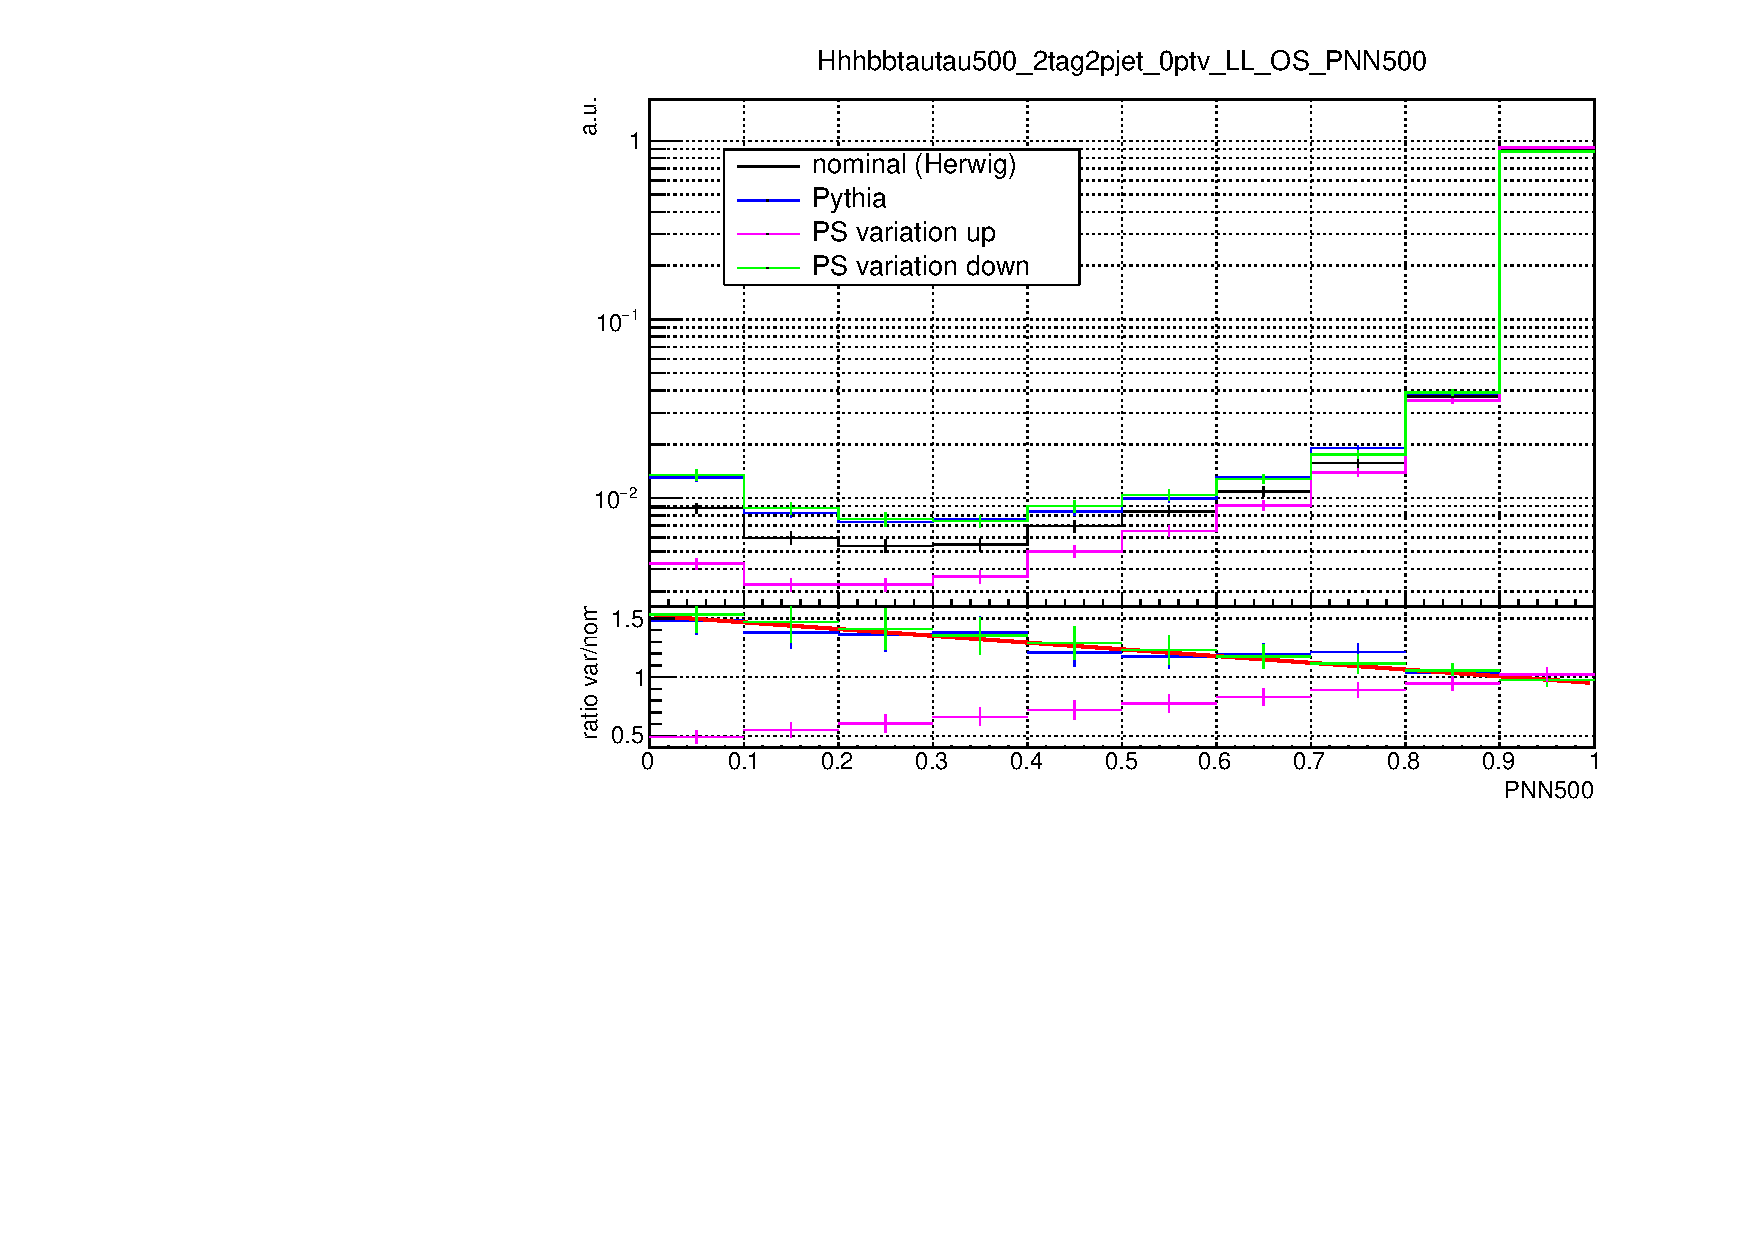
\includegraphics[width=.49\textwidth]{figures/systs/HadHad_Signal_500_PNN_SystsApplied_Fit_log.pdf}
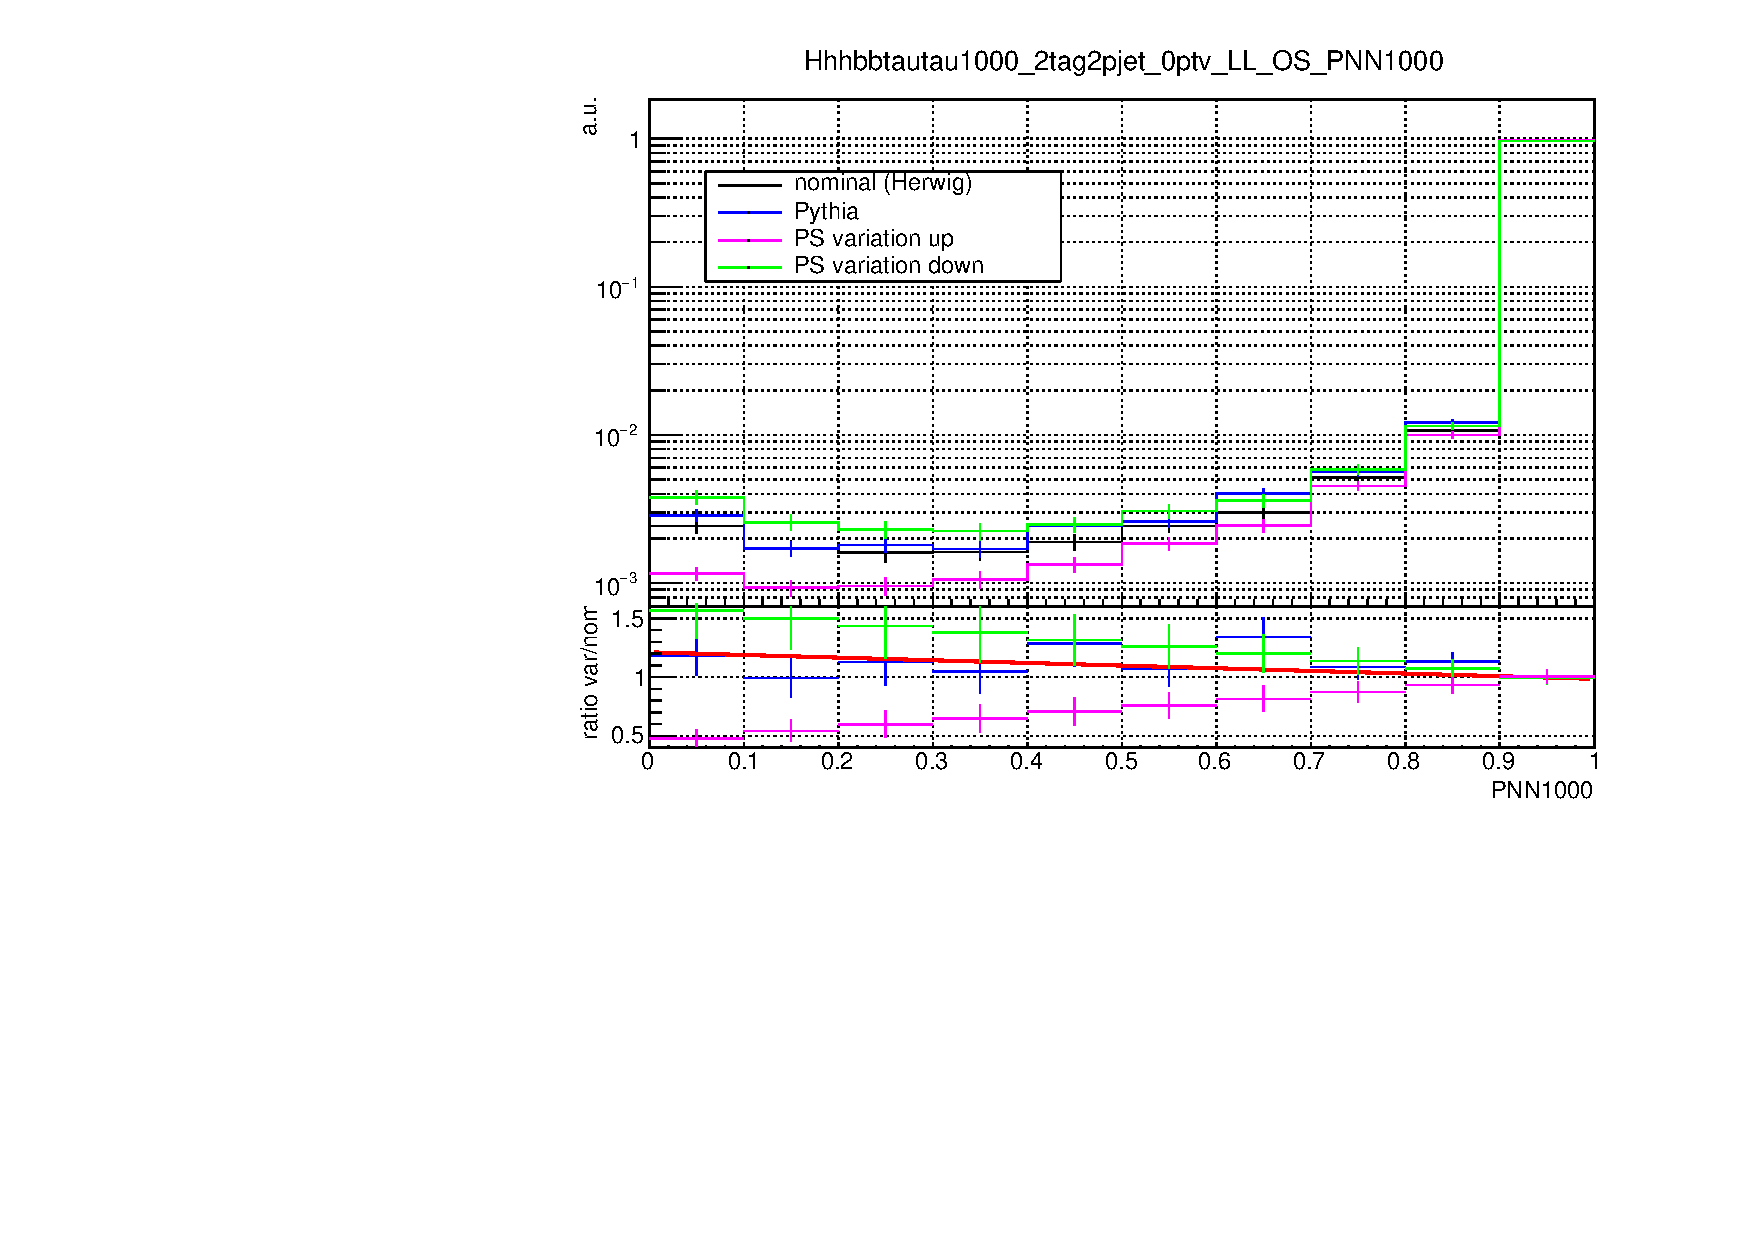
\includegraphics[width=.49\textwidth]{figures/systs/HadHad_Signal_1000_PNN_SystsApplied_Fit_log.pdf}
\caption{Comparison of the di-Higgs $bb\tau_{had}\tau_{had}$ signal PNN distributions obtained from the nominal (black) and alternative (blue) signal samples for the PS variations for the  $m_X= 500$ GeV (left) and the $m_X=1000$ GeV (right) mass points. A linear fit to the ratio of the two distributions is performed and shown in the lower panel of the figures (red line). The variations obtained from the linear function obtained from the $m_X= 500$ GeV fit are also shown in the figures (green and magenta).}
\label{fig:HadHadSignalSysts}
\end{figure}

In the $bb\tau_{lep}\tau_{had}$ channel the overall parton shower acceptance uncertainty on the normalisation is found to be 6\% for $m_X= 500$ GeV and 3\% for  $m_X=1000$ GeV in the SLT SR and 4\% for $m_X= 500$ GeV and 7\% for  $m_X=1000$ GeV in the LTT SR. Thus, a conservative 6\% uncertainty is applied on the normalisation for all mass points in the SLT SR and a conservative 7\% uncertainty is applied on the normalisation for all mass points in the LTT SR.

After taking out the normalisation effect, the acceptance uncertainty on the shape of the PNN distribution is evaluated. Figure~\ref{fig:LepHadSLTSignalSysts} and \ref{fig:LepHadLTTSignalSysts} show the comparisons of the PNN distributions obtained from the nominal (black) and alternative (blue) signal samples for the  $m_X= 500$ GeV and the $m_X=1000$ GeV mass points for the SLT and LTT SRs respectively. A linear fit to the ratio of the two distributions is performed to parameterise the shape variation as a function of the PNN score and shown in the lower panel of the figures (red line). The linear function in the PNN score obtained from the fit performed at $m_X= 500$ GeV has the largest slope so this function is used to obtain the templates for the variations for all mass points. 

The function used in the SLT SR is:

\begin{itemize}
\item Down variation = 1.82 - 0.95 * PNN Score.
\item Up variation = 0.18 + 0.95 * PNN Score;
\end{itemize}

The function used in the LTT SR is:

\begin{itemize}
\item Down variation = 1.84 - 1.01 * PNN Score;
\item Up variation = 0.16 + 1.01 * PNN Score.
\end{itemize}

The variations obtained from this linear function in the PNN score are also shown in the figures (green and magenta) showing that this variation covers the variation given by the alternative samples for the two available mass points in both SRs.

\begin{figure}
\centering
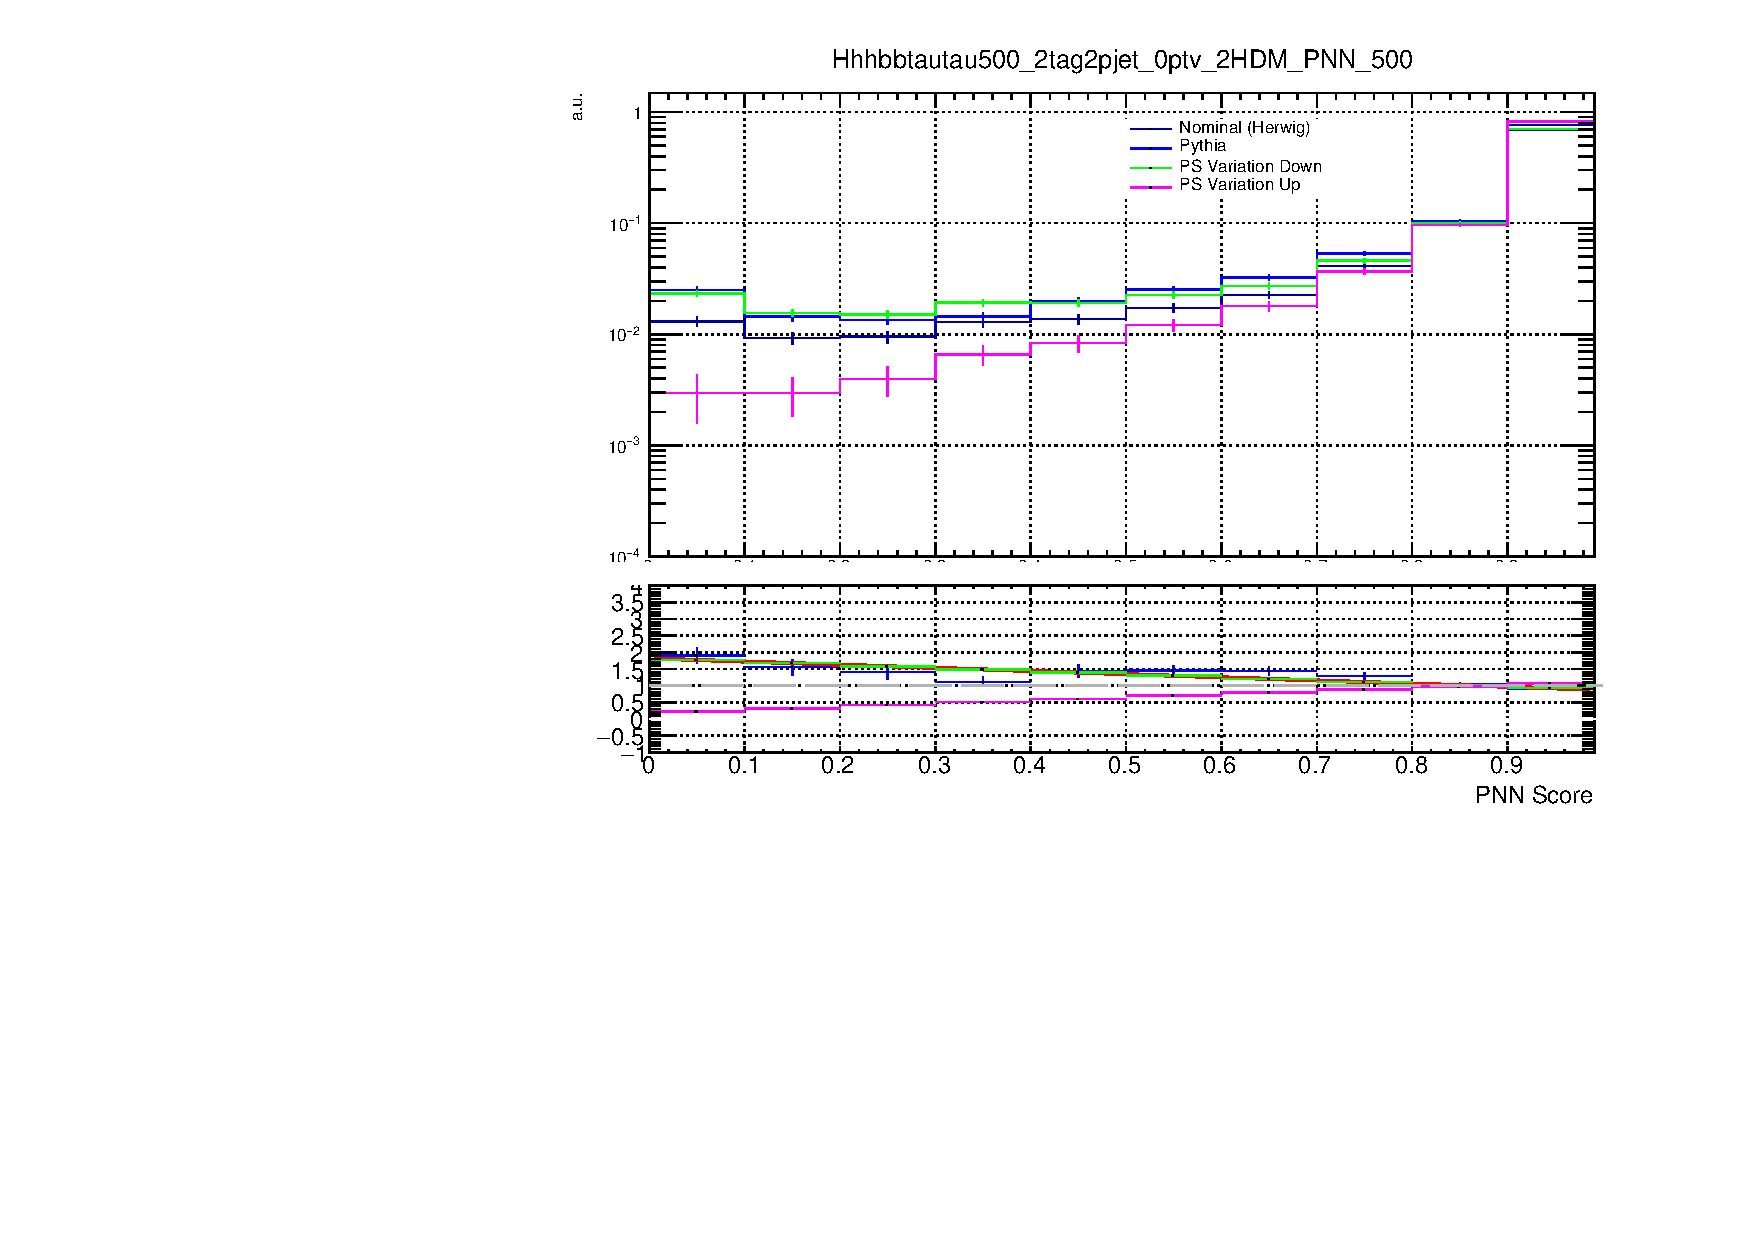
\includegraphics[width=.49\textwidth]{figures/systs/LepHad_Signal_SLT_500_psSysts_PNN_Fit_Logy.pdf}
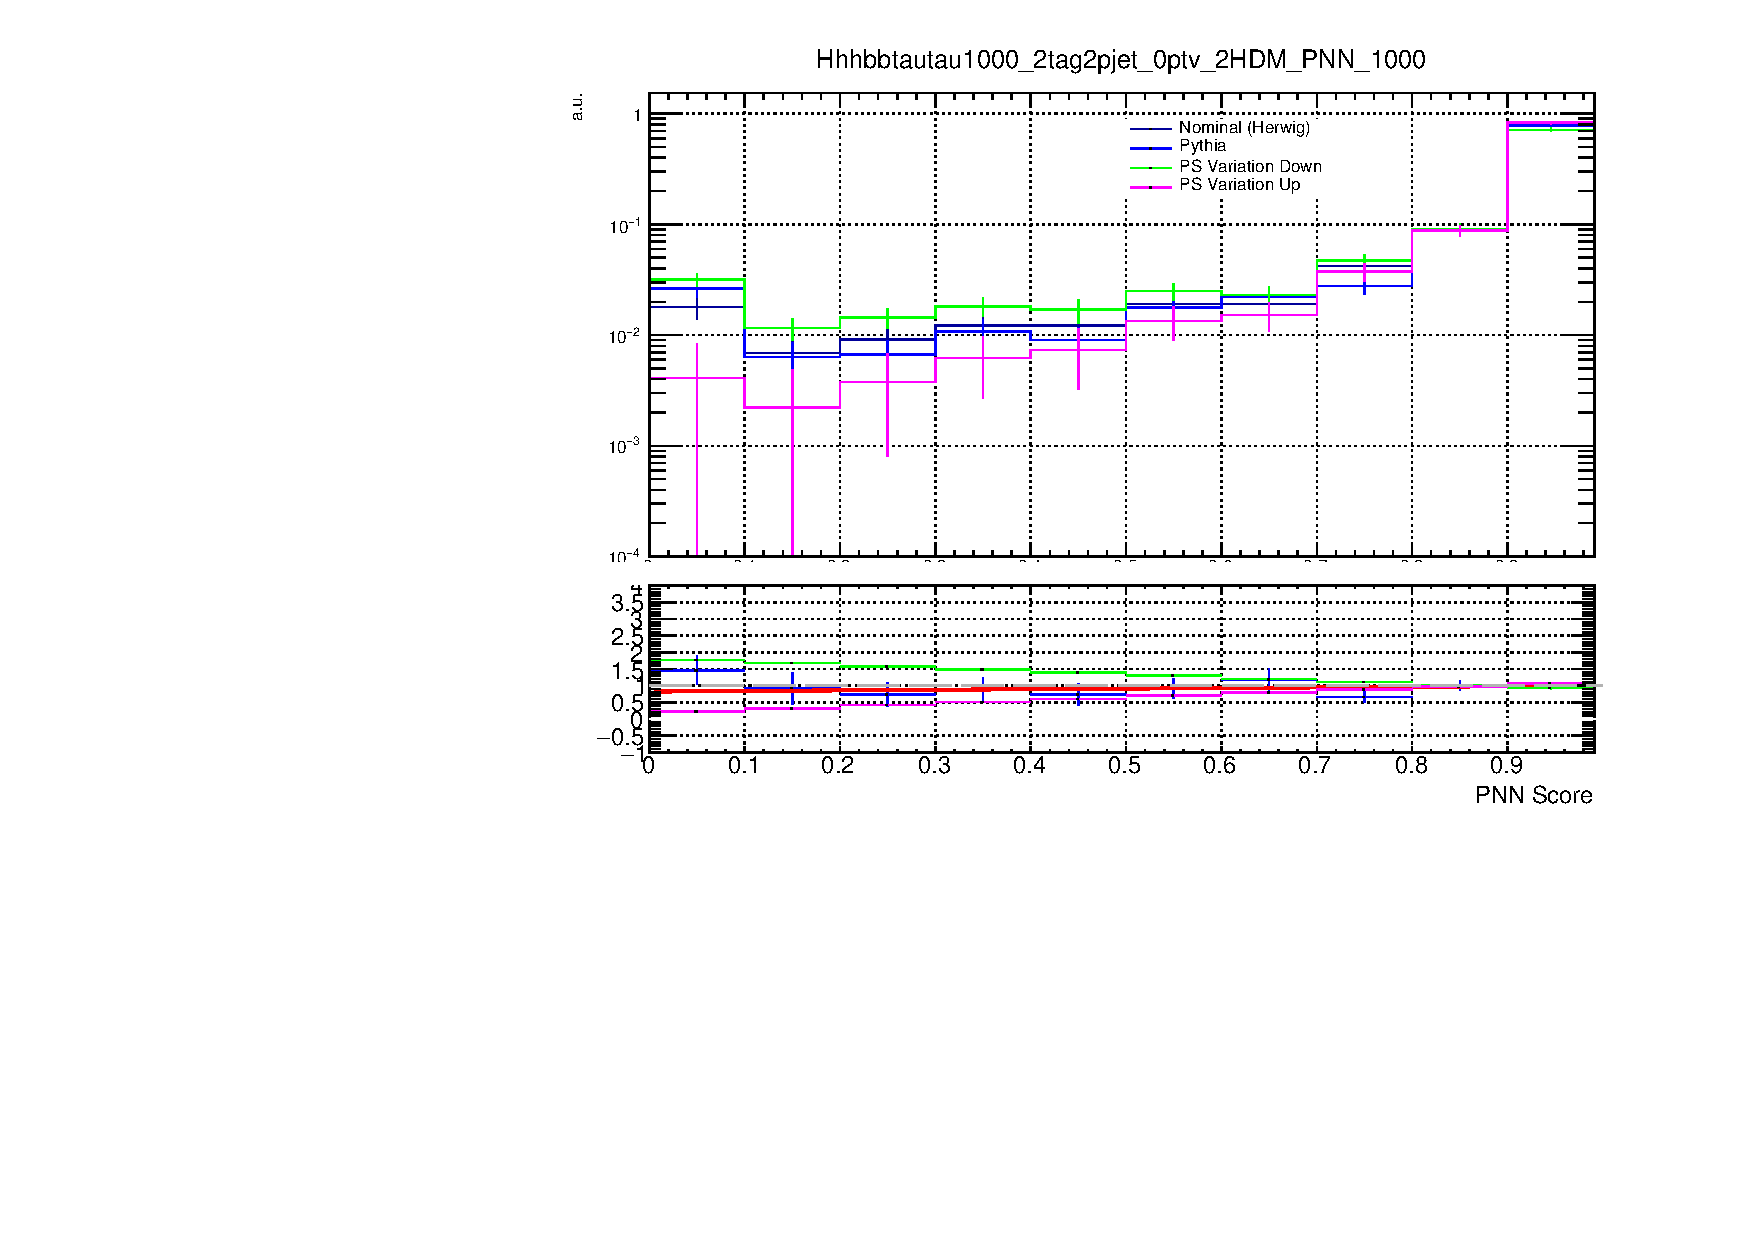
\includegraphics[width=.49\textwidth]{figures/systs/LepHad_Signal_SLT_1000_psSysts_PNN_Fit_Logy.pdf}
\caption{Comparison of the di-Higgs $bb\tau_{lep}\tau_{had}$ SLT signal PNN distributions obtained from the nominal (black) and alternative (blue) signal samples for the PS variations for the  $m_X= 500$ GeV (left) and the $m_X=1000$ GeV (right) mass points. A linear fit to the ratio of the two distributions is performed and shown in the lower panel of the figures (red line). The variations obtained from the linear function obtained from the $m_X= 500$ GeV fit are also shown in the figures (green and magenta).}
\label{fig:LepHadSLTSignalSysts}
\end{figure}

\begin{figure}
\centering
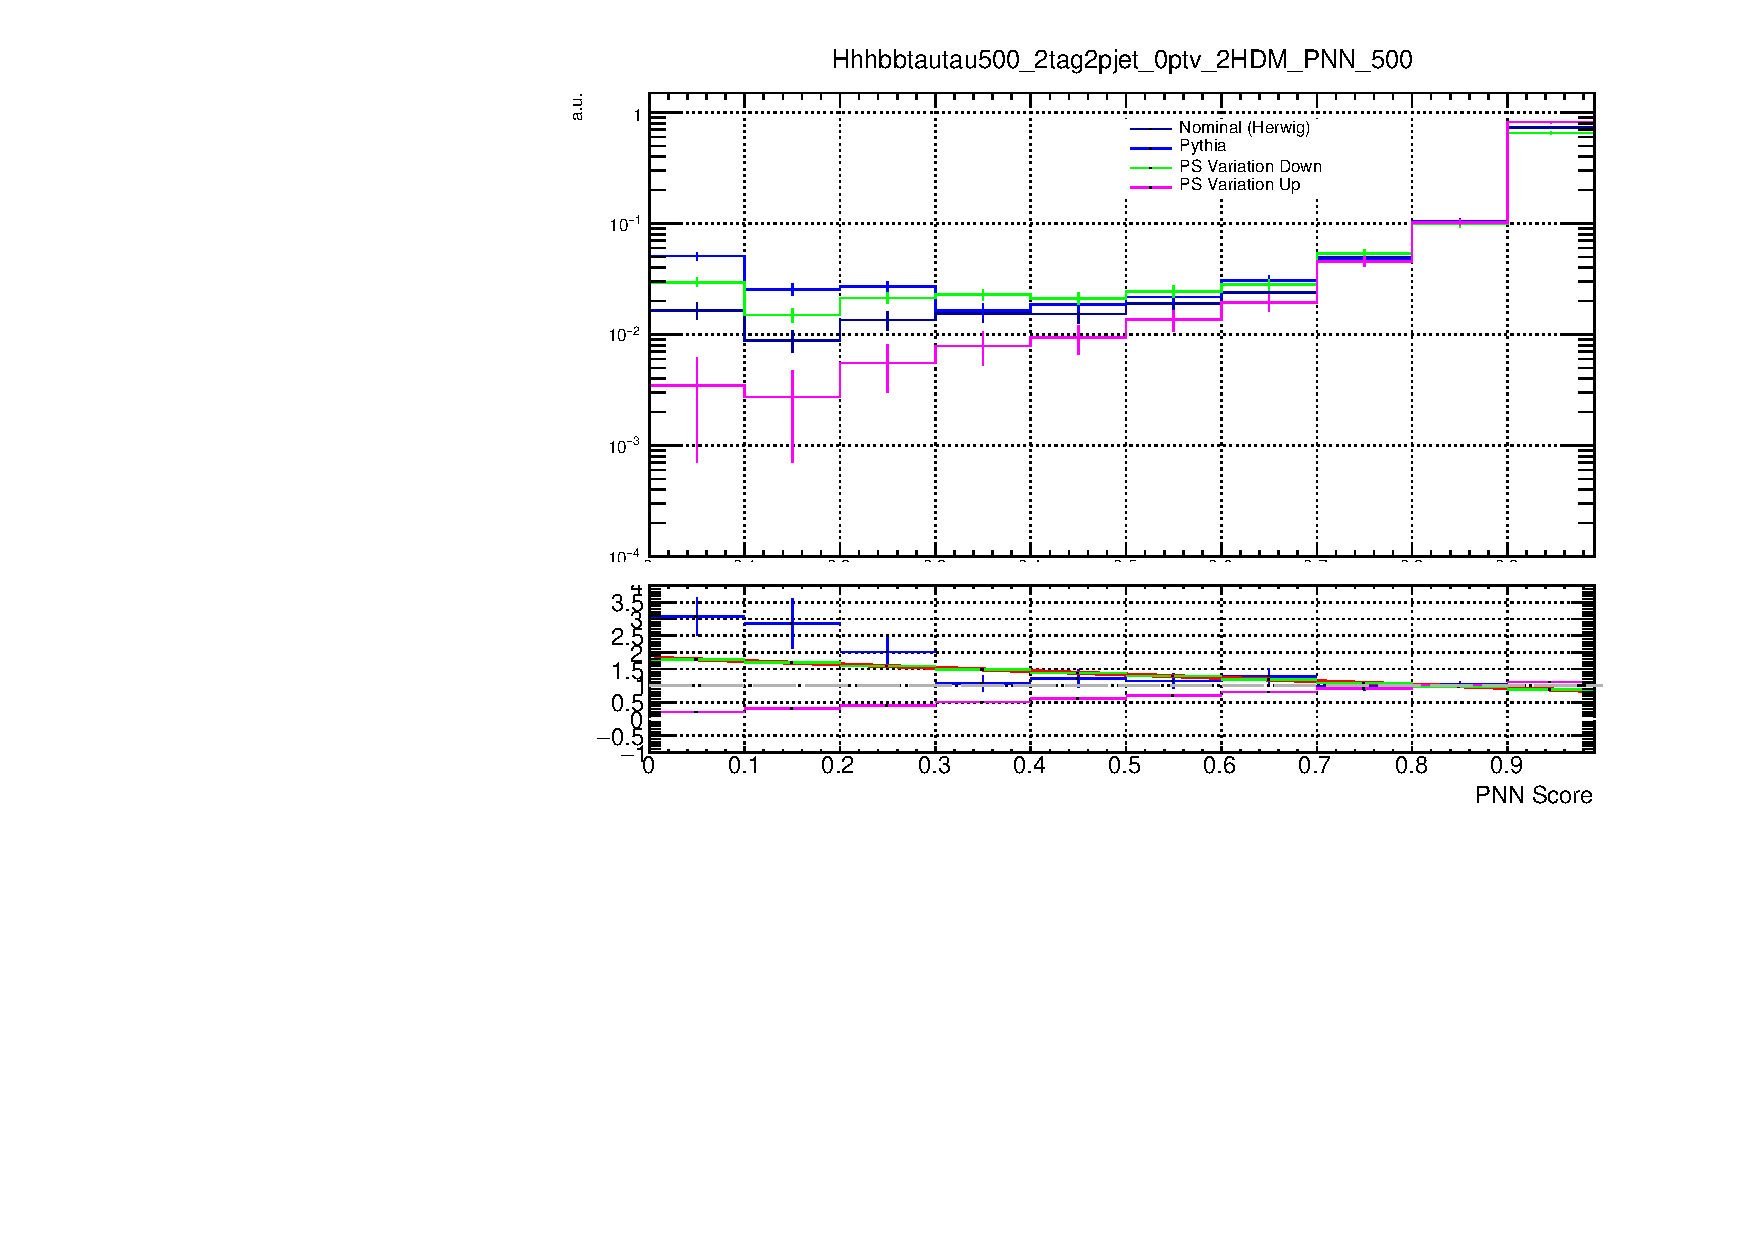
\includegraphics[width=.49\textwidth]{figures/systs/LepHad_Signal_LTT_500_psSysts_PNN_Fit_Logy.pdf}
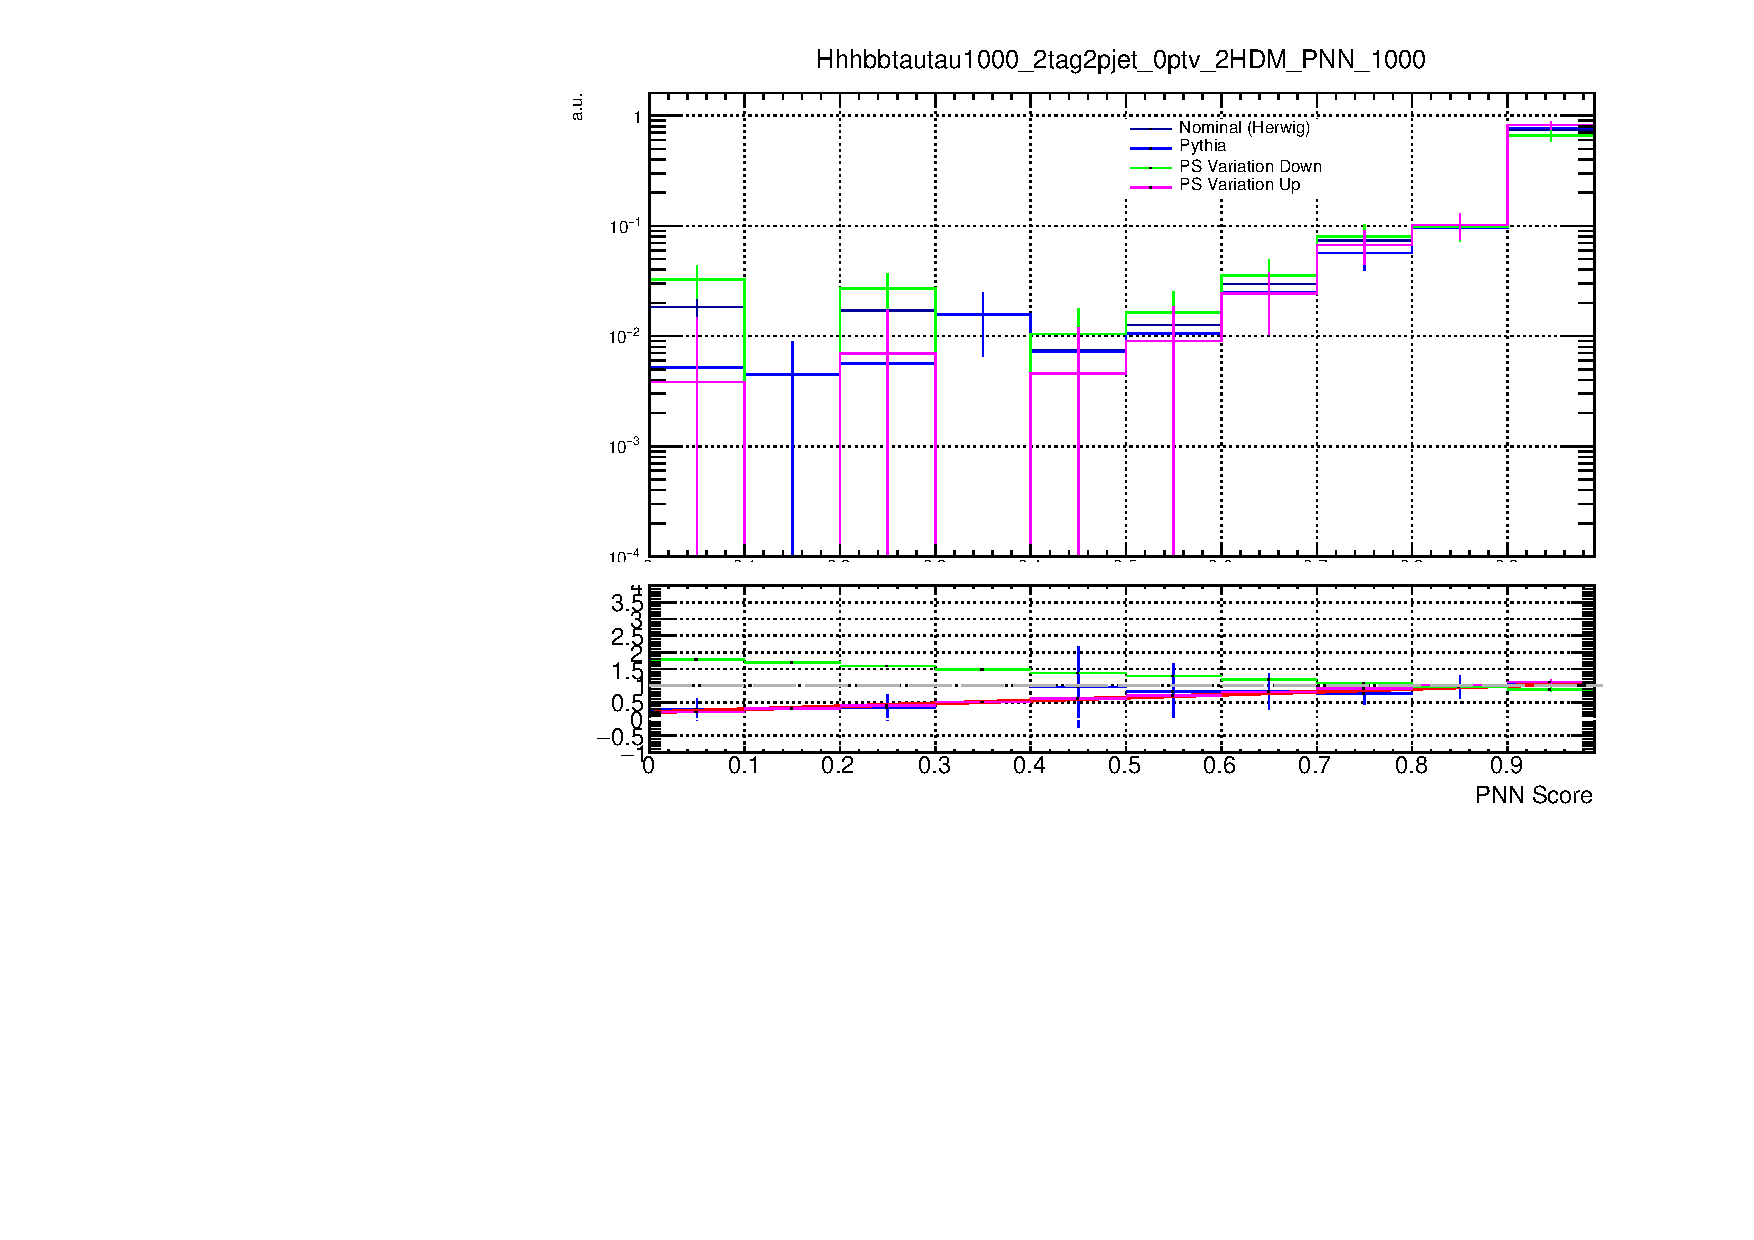
\includegraphics[width=.49\textwidth]{figures/systs/LepHad_Signal_LTT_1000_psSysts_PNN_Fit_Logy.pdf}
\caption{Comparison of the di-Higgs $bb\tau_{lep}\tau_{had}$ LTT signal PNN distributions obtained from the nominal (black) and alternative (blue) signal samples for the PS variations for the  $m_X= 500$ GeV (left) and the $m_X=1000$ GeV (right) mass points. A linear fit to the ratio of the two distributions is performed and shown in the lower panel of the figures (red line). The variations obtained from the linear function obtained from the $m_X= 500$ GeV fit are also shown in the figures (green and magenta).}
\label{fig:LepHadLTTSignalSysts}
\end{figure}

% PDFs and Scales below here

Scale, PDF and $\alpha_s$ uncertainties on signal are expected to be negligible compared to the parton shower uncertainties as it was found in the previous analysis and also in other di-Higgs channels (less than 1\%). They are checked using truth-level samples produced storing alternative weights for these settings. The on-the-fly MadGraphControl framework is used to generate LHE files including alrernative weights. Samples are produced for $m_X=500$ GeV and $m_X=1000$ GeV with 10000 events each. The generated truth-level samples are converted to TRUTH3 derivations and a truth-level analysis is implemented in order to mimic the selection of the analysis and select the same phase-space to evaluate these acceptance uncertainties.

For PDF and $\alpha_s$ variations, the NNPDF30\_ nlo\_s\_ 0118 uncertainty sets, consisting of 100 eigenvectors parameterising the uncertainties for all the PDFs and 1 parameter for the $\alpha_s$ variations, are used and are compared to the nominal NNPDF30\_ nlo\_s\_ 0118 to evaluate the size of the variations (as recommended by the Physics Modelling Group even if the nominal PDF used in the nominal sample is the NNPDF23\_ lo\_ as\_ 0130\_ qed set). These variations are combined following the recommendations~\cite{Butterworth:2015oua}, consisting in evaluating the PDF uncertainty $\delta_{PDF}$ by calculating the square root of the sum in quadrature of the 30 variations, evaluating the $\alpha_s$ uncertainty by taking the half difference between the same PDF set with two different $\alpha_s$ values, and then adding in quadrature the two contributions of $\delta_{PDF}$ and $\alpha_s$ uncertainties to obtain the total uncertainty. 

As alternative weights are available also for the alternative PDF sets MMHT2014nlo68clas118 and the CT14nlo these are also checked. Alternative weights are available also for the PDF4LHC\_ NLO\_ 30 uncertainty sets which consist of 30 eigenvectors for all the PDFs and 1 parameter for the $\alpha_s$ variations and these are also checked as a cross-check. 

Scale uncertainties are evaluated using the 7-point scale variations of the renormalisation ($\mu_R$) and the factorisation scale ($\mu_F$) which are combined by taking an envelope of all of the variations (as recommended by the Physics Modelling group). 

All acceptance uncertainties on the signal normalisation obtained in the different signal regions are shown in Table~\ref{sec:systs:tab:systematics_HHSignal_AcceptanceNumbers}.  

The PDF+$\alpha_s$ uncertainties obtained from the NNPDF30\_ nlo\_s\_ 0118 uncertainty set are found to be negligible compared to the Parton Shower uncertainties and the uncertainties obtained from PDF4LHC\_ NLO\_ 30 uncertainty set and from the two alternative PDF sets are well within the NNPDF30\_ nlo\_s\_ 0118 variations. The effect of PDF+$\alpha_s$ uncertainties on the shapes of the PNN input variables is also checked and found to be negligible as shown in Appendix~\ref{subsec:appendix_systs_signalsysts}. Thus, the PDF+$\alpha_s$ uncertainties on signal are neglected in the analysis. 

The scale uncertainties are also found to be negligible compared to the Parton Shower uncertainties and their effect on the shapes of the PNN input variables is also is also checked and found to be negligible as shown in Appendix~\ref{subsec:appendix_systs_signalsysts}. Thus, the scale uncertainties on signal are neglected in the analysis. 

As the resonant samples are generated with AF2 for masses up to 1 TeV (from \SI{1.1}{\TeV}
full simulation is used), the difference between the AF2 samples and
the full simulation samples is checked.  

In the \lephad channel, the
check is done using the 400 GeV mass point sample of 2017 and 2018
(mc16d, mc16e) MC.  The difference is less than 1\% in the SLT channel
and 2.9\% in the LTT channel, and there is no obvious shape
difference between the two types of simulation, as shown in
Figure~\ref{fig:Lephad_resonant_AF2_VS_FS}. 
As discussed in the following paragraph, it was found that the larger difference in acceptance times efficiency in 
LTT is originating from the \tauhad 
triggers for which no dedicated recommendations for AF2 exist.
Therefore a 3\% acceptance uncertainty is assigned to LTT of all signal
samples simulated with AF2 (up to 1TeV mass point).

\begin{figure}
  \centering
  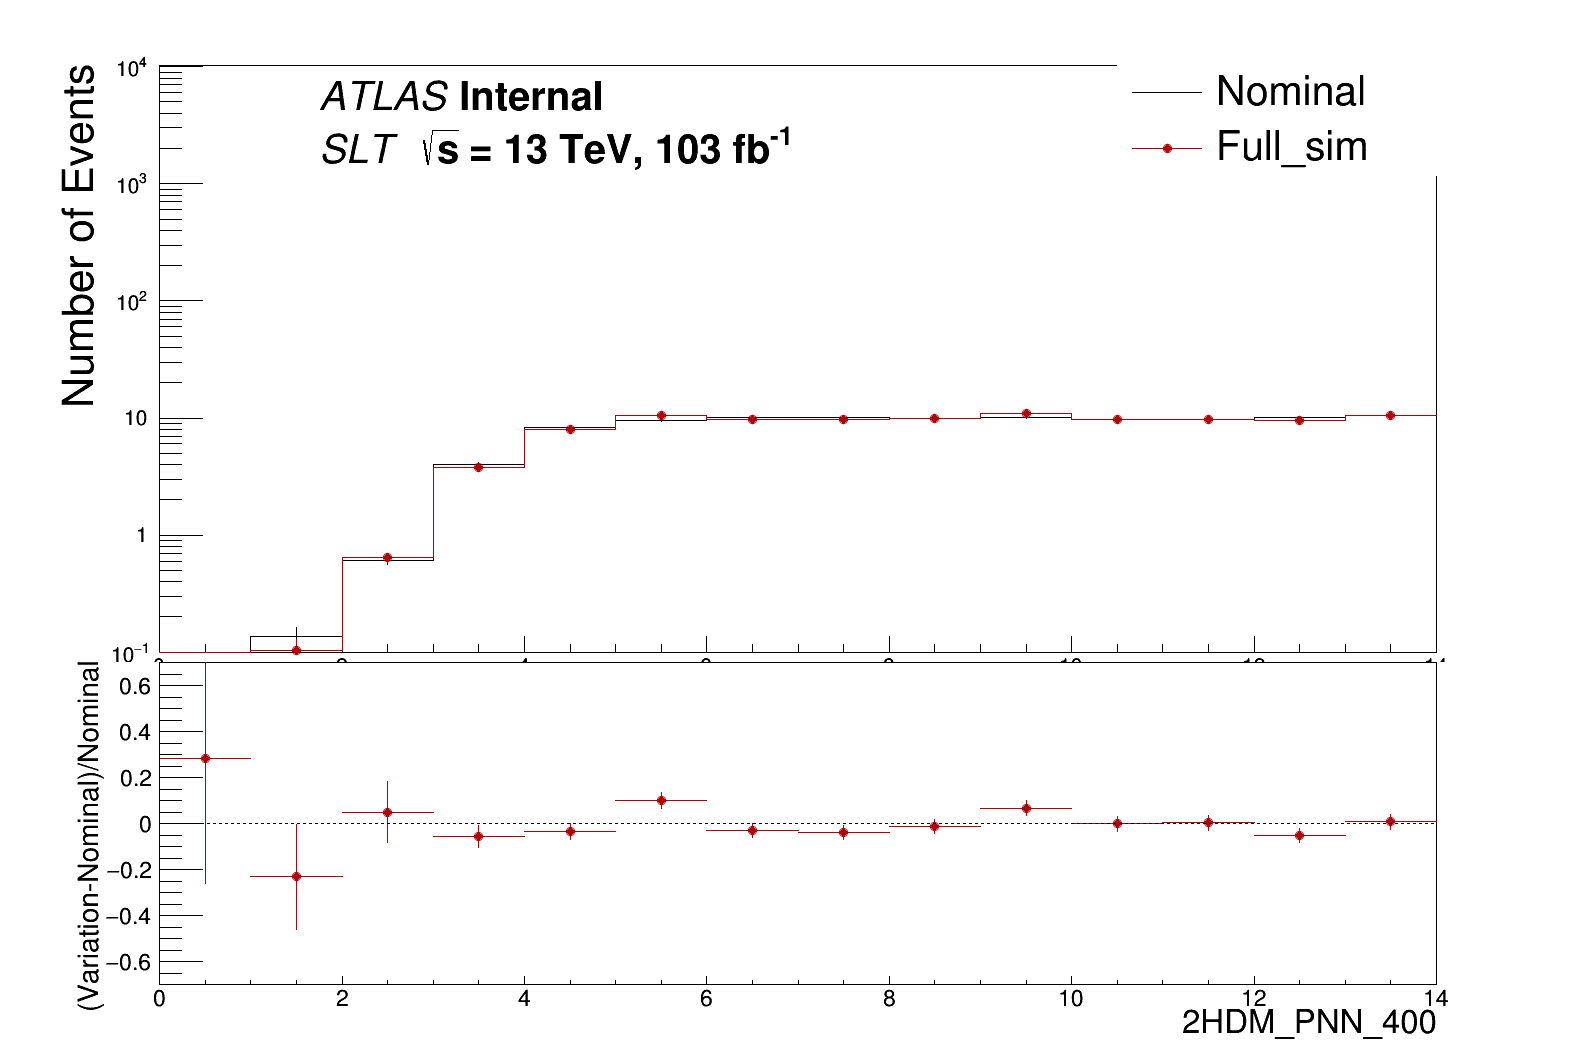
\includegraphics[width=.49\textwidth]{figures/lephad_modelling_systs/SLT/signal_AF2_check/limit_binning_2HDM_PNN_400_Norm.png}
  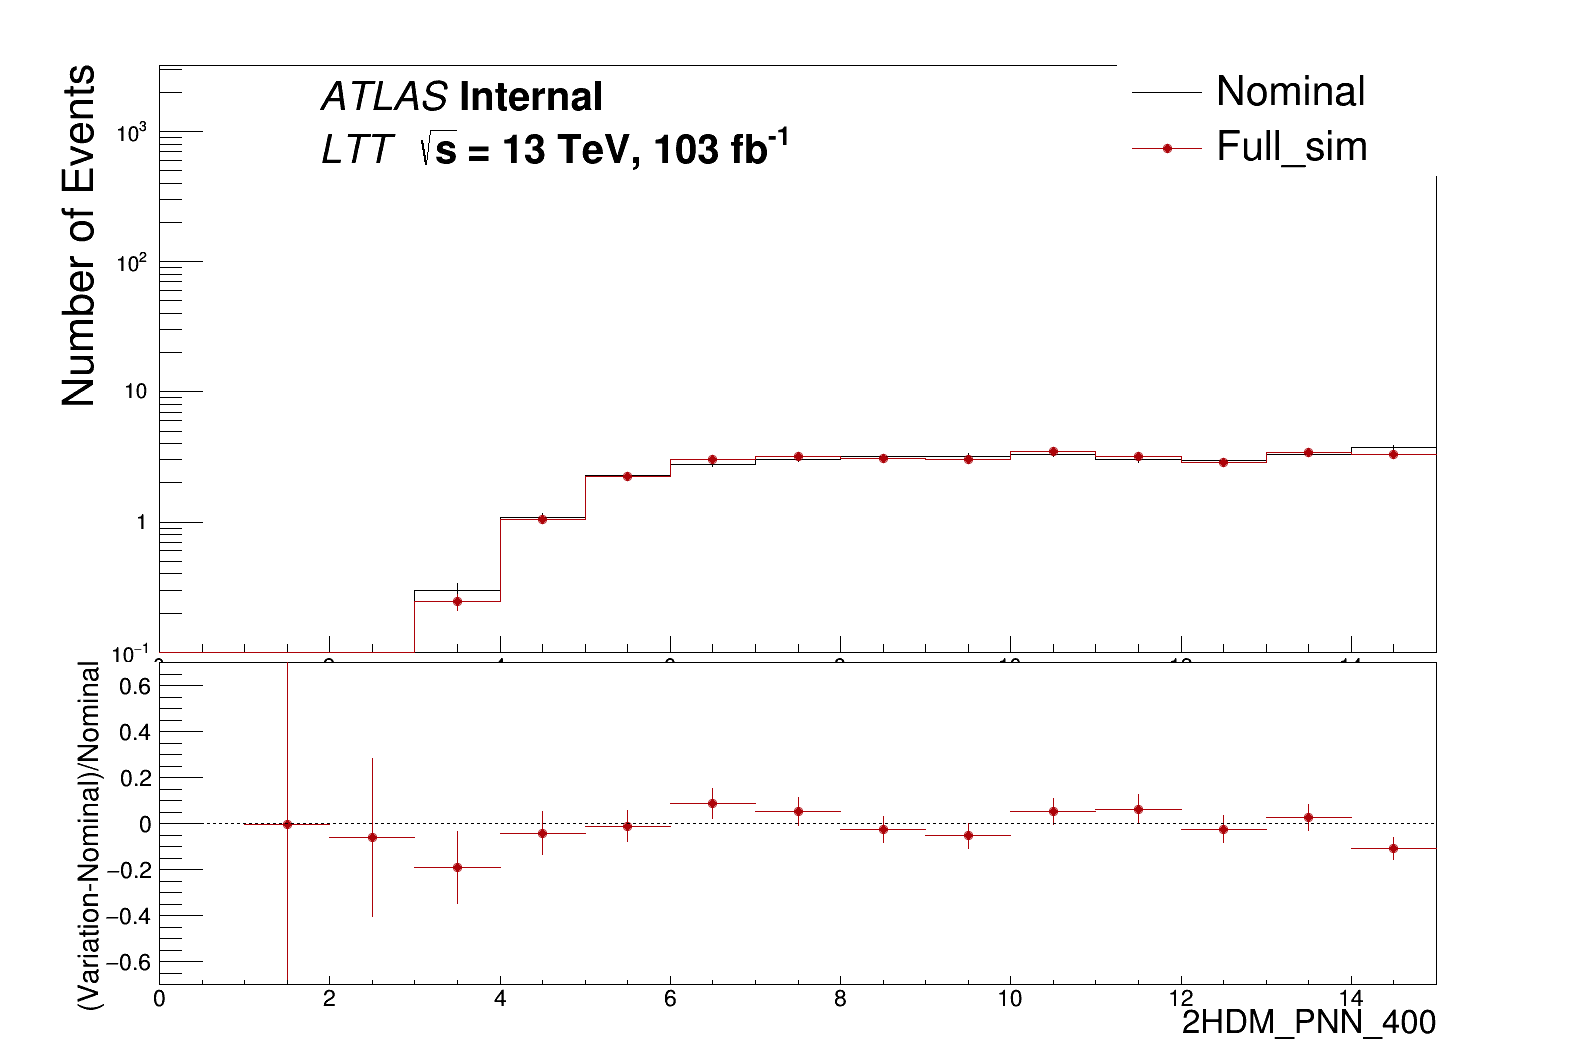
\includegraphics[width=.49\textwidth]{figures/lephad_modelling_systs/LTT/signal_AF2_check/limit_binning_2HDM_PNN_400_Norm.png}
  \caption{Comparison of the di-Higgs \lephad signal PNN distributions obtained from the nominal (AF2)
    and alternative (full simulation) signal samples for the  $m_X= 400$ GeV for the
    SLT (left) and the LTT (right) channel. The binning is the same as the final fit binning.
  }
  \label{fig:Lephad_resonant_AF2_VS_FS}
\end{figure}

In the \hadhad-channel the acceptance of the resonant signal is
compared between full- and fast-simulation using the \SI{400}{\GeV}
$\text{X} \to \text{HH}$ simulated sample using MC16A
only\footnote{The primary AODs for the full-simulation MC16D and MC16E
  samples were unfortunately deleted due to the obsolesence procedure
  and thus were not available for this study.}. A statistically
significant deviation of more than three standard deviations is
observed in the overall acceptance times efficiency of the \hadhad SR selection. The
fast-simulation tends to overestimate the signal yield by 6.5~\% in
the \hadhad SR. Comparing the cutflows between fast- and
full-simulation (c.f.\ \Cref{tab:cutflow_fullsim_fastsim_hadhad}), it
was determined that this discrepancy is originating from the \tauhad
triggers for which no dedicated recommendations for AF2 exist. The
distribution of the final discriminant (PNN400) was compared for both
samples which showed no discernable impact on the shape of the
distribution. Additionally, the impact was compared between the STT
and DTT trigger-channels showing equal impact in both. Therefore, a
6.5~\% normalization uncertainty is assigned to all signal samples
simulated using AF2 (i.e.\ up to the 1 TeV mass
point). 

\begin{table}
\centering
\small
\begin{tabular}{|c|c|c|c|c|}
\hline
Process X, GeV& HadHad & LepHad SLT  & LepHad LTT & Description\\
\hline
$m_{X}= 400$ & 0.065 &  <0.01 & 0.029 & AF2\\
$m_{X}= 500$ & 0.093 &  0.06 & 0.05 & Parton Shower\\
$m_{X}= 500$ & 0.001 &  0.0033 & 0.023 & PDF+$\alpha_s$ from NNPDF30\_ nlo\_s\_ 0118\\
$m_{X}= 500$ & 0.00013 &   0.00031 &  0.00051 & Alt. PDF from MMHT2014nlo68clas118\\ %UPDATE HADHAD
$m_{X}= 500$ & 0.00029 &  0.000063 &  0.00046 & Alt. PDF from CT14nlo\\ 
$m_{X}= 500$ & 0.00055 &  0.00078 &  0.0020 & PDF+$\alpha_s$ from PDF4LHC\\ 
$m_{X}= 500$ & 0.00015 &  0.00048 &  0.0012 & Scales \\
$m_{X}= 1000$ & 0.062 &  0.03 &  0.07 & Parton shower\\
$m_{X}= 1000$ & 0.00077 &  0.0094 &  0.029 & PDF+$\alpha_s$ from NNPDF30\_ nlo\_s\_ 0118\\
$m_{X}= 1000$ & 0.00007 &  0.00034 &   0.0009 & Alt. PDF from MMHT2014nlo68clas118\\ %UPDATE HADHAD
$m_{X}= 1000$ & 0.00008 &   0.00029 &  0.0024 & Alt. PDF from CT14nlo\\ 
$m_{X}= 1000$ & 0.00051 &   0.0013 &  0.0069 & PDF+$\alpha_s$ from PDF4LHC\\ 
$m_{X}= 1000$ & 0.00015 &   0.00067 &  0.0019  & Scales \\
\hline
\end{tabular}
\caption{List and relative size of the ggF HH resonant signal acceptance uncertainties in the individual signal regions.}
\label{sec:systs:tab:systematics_HHSignal_AcceptanceNumbers}
\end{table}


%PDF+alphas HadHad
%n the di-Higgs $bb\tau_{had}\tau_{had}$ channel the overall PDF+$\alpha_s$ acceptance uncertainty on the normalisation is found to be 0.10\% for $m_X= 500$ GeV and 0.077\% for  $m_X=1000$ GeV using the NNPDF30\_ nlo\_s\_ 0118 uncertainty sets. 
%As alternative weights are available also for the alternative PDF sets MMHT2014nlo68clas118 and the CT14nlo these are also checked. The largest variation comes from the CT14nlo PDF set and it is of 0.029\% for $m_X= 500$ GeV and 0.008\% for $m_X= 1000$ GeV, so well within the NNPDF30\_ nlo\_s\_ 0118 variations and thus neglected.  
%Alternative weights are available also for the PDF4LHC\_ NLO\_ 30 uncertainty sets which consist of 30 eigenvectors for all the PDFs and 1 parameter for the $\alpha_s$ variations and these are also checked as a cross-check. The PDF+$\alpha_s$ acceptance uncertainty on the normalisation is found to be 0.0055\% for $m_X= 500$ GeV and 0.051\% for  $m_X=1000$ GeV using the PDF4LHC\_ NLO\_ 30 uncertainty sets (smaller than the uncertainties from the NNPDF30\_ nlo\_s\_ 0118 uncertainty sets).
%The effect of PDF+$\alpha_s$ uncertainties on the shapes of the PNN input variables is also checked and found to be negligible as shown in Appendix~\ref{subsec:appendix_systs_signalsysts}.
%Thus, the PDF+$\alpha_s$ uncertainties on signal are neglected in the analysis. 

%Scale HadHad
%In the di-Higgs $bb\tau_{had}\tau_{had}$ channel the scale acceptance uncertainty on the normalisation is found to be 0.015\% for both $m_X= 500$ GeV and  $m_X=1000$ GeV. The effect of the scale uncertainties on the shapes of the PNN input variables is also checked and found to be negligible as shown in Appendix~\ref{subsec:appendix_systs_signalsysts}.
%Thus, the scale uncertainties on signal are neglected in the analysis.

\subsubsection{Non-resonant signal}

\paragraph{ggF non-resonant}

Acceptance uncertainties on the non-resonant production of di-Higgs via ggF are derived using the recommendations from PMG.

The parton shower uncertainties are estimated by comparing the nominal samples showered with Pythia8 to alternative samples showered with Herwig7. The alternative samples used for the parton shower uncertainties are reported in Table~\ref{sec:systs:tab:systematics_NonRessignalsamples}.


\begin{table}
\centering
\begin{tabular}{|c|c|}
\hline
DSID & Name\\
\hline
600023 & PhH7EG\_PDF4LHC15\_HHbbtautauHadHad\_cHHH01d0\\
600024 & PhH7EG\_PDF4LHC15\_HHbbtautauHadHad\_cHHH10d0\\
600029 & PhH7EG\_PDF4LHC15\_HHbbtautauLepHad\_cHHH01d0\\
600030 & PhH7EG\_PDF4LHC15\_HHbbtautauLepHad\_cHHH10d0\\
\hline
\end{tabular}
\caption{List of alternative di-Higgs non-resonant signal samples for PS uncertainties.
}
\label{sec:systs:tab:systematics_NonRessignalsamples}
\end{table}


In the \hadhad channel the overall parton shower acceptance uncertainty on the normalisation is found to be 4.3\% and 5.1\% for the SM non-resonant signal and for the $\kappa_\lambda=10$ non-resonant signal, respectively.  In the \lephad channel it is found to be for the SM signal 7.6\% in SLT and 7.5\% in LTT.

Uncertainties from PDF, $\alpha_s$ and scales are evaluated using alternative weights available in the nominal samples.

PDF and $\alpha_s$ uncertainties are evaluated using the alternative weights for the PDF4LHC\_ NLO\_ 30 uncertainty sets which consist of 30 eigenvectors for all the PDFs and 1 parameter for the $\alpha_s$ variations. These variations are combined following the recommendations~\cite{Butterworth:2015oua}, consisting in evaluating the PDF uncertainty $\delta_{PDF}$ by calculating the square root of the sum in quadrature of the 30 variations, evaluating the $\alpha_s$ uncertainty by taking the half difference between the same PDF set with two different $\alpha_s$ values, and then adding in quadrature the two contributions of $\delta_{PDF}$ and $\alpha_s$ uncertainties to obtain the total uncertainty. 

In the \hadhad channel PDF+$\alpha_s$ uncertainties are found to be 0.1\% and 0.7\% on the non-resonant SM signal and the non-resonant $\kappa_\lambda$ signal respectively and are thus neglected in the analysis as they are below 1\%. In the \lephad channel they are found to be for the SM signal 0.6\% in SLT and 0.7\% in LTT and are also neglected in the analysis.

Scale uncertainties are evaluated using the 7-point scale variations of the renormalisation ($\mu_R$) and the factorisation scale ($\mu_F$) which are combined by taking an envelope of all of the variations (as recommended by the Physics Modelling group). 

In the \hadhad channel the scale uncertainties are found to be 1.4\% on both the non-resonant SM signal and the non-resonant $\kappa_\lambda$ signal respectively and are included in the analysis.  In the \lephad channel they are found to be for the SM signal 1.2\% in SLT and 1\% in LTT.

After taking out the normalisation effects, shape effects were checked on the MVA score distributions and found to be negligible as reported in Appendix~\ref{subsec:appendix_systs_signalsysts} and therefore are not considered in the analysis.



\begin{table}
\centering
\small
\begin{tabular}{|c|c|c|c|c|}
\hline
Process & HadHad & LepHad SLT & LepHad LTT & Description\\
\hline
SM  & 0.043 &  0.076 & 0.075 & Parton Shower\\
SM & 0.0010 &  0.0061 &  0.0072 & PDF+$\alpha_s$ from PDF4LHC\\ 
SM & 0.014 &  0.012 &  0.010 & Scales \\
$\kappa_\lambda=10$ & 0.051 &  ? & ? & Parton Shower\\
$\kappa_\lambda=10$ & 0.007 &  ? &  ? & PDF+$\alpha_s$ from PDF4LHC\\ 
$\kappa_\lambda=10$ & 0.014 &  ? &  ? & Scales \\
\hline
\end{tabular}
\caption{List and relative size of ggF HH non-resonant signal acceptance uncertainties in the individual signal regions.}
\label{sec:systs:tab:systematics_HHNonResSignal_AcceptanceNumbers}
\end{table}

Cross section uncertainties are also included, with values from \href{https://twiki.cern.ch/twiki/bin/view/LHCPhysics/LHCHWGHH?redirectedfrom=LHCPhysics.LHCHXSWGHH#Latest_recommendations_for_gluon}{\underline{LHCHHWG}} recommendations, shown in Table~\ref{sec:systs:tab:systematics_HHNonResSignal_XSecNumbers}.

\begin{table}
\centering
\small
\begin{tabular}{|c|c|}
\hline
Source & Uncertainty\\
\hline
%Scale & -0.05, +0.022\\
%PDF & 0.021\\
%$\alpha_s$ & 0.021\\
%Mtop approx.  & 0.026\\
Combined Scale+MTop & -0.23, +0.06\\
Combined PDF+$alpha_s$ & -0.03, +0.03\\
\hline
\end{tabular}
\caption{List and relative size of ggF HH non-resonant SM signal cross section uncertainties.}
\label{sec:systs:tab:systematics_HHNonResSignal_XSecNumbers}
\end{table}


\paragraph{VBF non-resonant}

Acceptance uncertainties on the non-resonant production of di-Higgs
via VBF are derived using the recommendations from PMG. 

The acceptance uncertainties from missing higher orders are derived by
varying the factorization $\mu_\text{F}$ and renormalization scale
$\mu_\text{R}$ independently and coherently resulting in 7 settings
for the scales (including the nominal). 

The effect of these variations
on the normalization of the signal in the \hadhad-channel is
negligible. A small (less than 2 \%) shape-impact on the final
discriminant in the \hadhad-channel is observed
in~\Cref{fig:vbf_uncertainties_scale_pdf}. This shape is directly
propagated using the internal weights to the fit. 
The signal acceptance uncertainty due to scale variations is derived as 0.86\% (0.63\%) for the \lephad SLT (LTT) channel.
Corresponding distributions can be found in~\Cref{fig:lephad_vbf_scale_pdf}.


The PDF+\alphas uncertainties are derived using the error set of the
NNPDF30NLO PDF used for the generation of the signal
sample. Additionally, the value of \alphas is varied from 0.118 to
0.119 and 0.117 to evaluate the impact of the choice of \alphas. These
two sources of uncertainties are combined by adding them in
quadrature. 

Both in the \hadhad and \lephad channels, the PDF+\alphas uncertainty shows
no shape impact on the final discriminants
(c.f.~\Cref{fig:vbf_uncertainties_scale_pdf} for the \hadhad and ~\Cref{fig:lephad_vbf_scale_pdf} for the \lephad channels, respectively). The overall norm
uncertainty is well below 1\% therefore a conservative uncertainty of
1\% (max fluctuation observed) is assigned to the non-resonant production of di-Higgs via VBF in
the \hadhad-channel. In the \lephad channel, this uncertainty is calculated as 0.15\% (0.23\%) for the SLT (LTT) channel,
and therefore found negligible.

\begin{figure}[htbp]
  \centering

  \subfloat[]{\includegraphics[width=0.5\textwidth]{figures/systs/hadhad_vbf/scale}}%
  \subfloat[]{\includegraphics[width=0.5\textwidth]{figures/systs/hadhad_vbf/pdf}}

  \caption{Impact of the 7-point scale variations on the final
    discriminant (SMBDT) in the SR of the \hadhad-channel (a) and the
    PDF+\alphas uncertainties (b). The shape-impact of the
    factorization scale variation is propagated using the internal
    weights to the final discriminant.}
  \label{fig:vbf_uncertainties_scale_pdf}
\end{figure}

Finally, the nominal VBF signal sample showered with Pythia8 is
compared to an alternative sample using Herwig7 for the parton
shower. The alternative PS shows no significant
shape impact on the final discriminants, therefore a 3\% uncertainty
on the normalisation is assigned in the \hadhad channel, whereas a 6.3\% (2.1\%) uncertainty 
is assigned in the SLT (LTT) \lephad channel. The comparison of parton shower
algorithms is shown in~\Cref{fig:vbf_uncertainties_ps} and ~\Cref{fig:lephad_vbf_ps}, 
for the \hadhad and \lephad channels, respectively.

\begin{figure}[htbp]
  \centering

  \subfloat[]{\includegraphics[width=0.5\textwidth]{figures/systs/lephad_vbf/VBFNonRes_Scale_SM_NN_SLT.pdf}}
  \subfloat[]{\includegraphics[width=0.5\textwidth]{figures/systs/lephad_vbf/VBFNonRes_Scale_SM_NN_LTT.pdf}}\\
  \subfloat[]{\includegraphics[width=0.5\textwidth]{figures/systs/lephad_vbf/VBFNonRes_PDF_SM_NN_SLT.pdf}}	
  \subfloat[]{\includegraphics[width=0.5\textwidth]{figures/systs/lephad_vbf/VBFNonRes_PDF_SM_NN_LTT.pdf}}
  \caption{Impact of the 7-point scale variations on the final
    discriminant (SMNN) in the SR of the \lephad SLT channel (a) in the LTT channel (b), 
    and the PDF+\alphas uncertainties in the SLT channel (c), in the LTT channel (d).}
  \label{fig:lephad_vbf_scale_pdf}
\end{figure}


\begin{figure}[htbp]
  \centering

  \includegraphics[width=0.5\textwidth]{figures/systs/hadhad_vbf/ps}

  \caption{Comparison of the alternative parton shower (Herwig7, red)
    with the nominal VBF signal sample (Pythia8, black) in the SR of
    the \hadhad-channel. To compare the shape-impact of this source of
    uncertainty, both histograms are normalised to the same integral
    before comparison. The uncertainty assigned due to PS algorithm is
    rounded up to 3 \% so that it also covers the deviations seen in
    the most significant SMBDT bins (note the difference in these bins
    before removing the normalisation from both histograms is
    $\approx \SI{3}{\percent}$) since this is where the analysis is
    most sensitive to the VBF HH contribution.}
\label{fig:vbf_uncertainties_ps}
\end{figure}

\begin{figure}[htbp]
  \centering

  \subfloat[]{\includegraphics[width=0.5\textwidth]{figures/systs/lephad_vbf/VBFNonRes_PS_SM_NN_SLT.pdf}}
  \subfloat[]{\includegraphics[width=0.5\textwidth]{figures/systs/lephad_vbf/VBFNonRes_PS_SM_NN_LTT.pdf}}

  \caption{Comparison of the alternative parton shower (Herwig7, red)
    with the nominal VBF signal sample (Pythia8, black) in the SR of
    the \lephad SLT channel (a), in the LTT channel (b). The uncertainty assigned due to PS algorithm is
    6.3\% (2.1\%) for the SLT (LTT) channel, which covers the deviations seen in
    the most significant SMNN bins.}
\label{fig:lephad_vbf_ps}
\end{figure}



\begin{table}
\centering
\small
\begin{tabular}{|c|c|c|c|c|}
\hline
Process & HadHad & LepHad SLT & LepHad LTT & Description\\
\hline
SM  & 3\,\% & 6.3\,\% & 2.1\,\% & Parton Shower\\
SM & 1\,\% &  0.15\,\% &  0.23\,\% & PDF+$\alpha_s$ from NNPDF30NLO errorset\\
SM & $\approx 0\,\%$ &  0.86\,\% &  0.63\,\% & Scales \\
\hline
\end{tabular}
\caption{List and relative size of VBF HH non-resonant signal acceptance uncertainties in the individual signal regions.}
\label{sec:systs:tab:systematics_HHNonResSignalVBF_AcceptanceNumbers}
\end{table}

Cross section uncertainties are also included, with values from \href{https://twiki.cern.ch/twiki/bin/view/LHCPhysics/LHCHWGHH?redirectedfrom=LHCPhysics.LHCHXSWGHH#Latest_recommendations_for_gluon}{\underline{LHCHHWG}} recommendations, shown in Table~\ref{sec:systs:tab:systematics_HHNonResSignalVBF_XSecNumbers}.

\begin{table}
\centering
\small
\begin{tabular}{|c|c|}
\hline
Source & Uncertainty\\
\hline
Scale & -0.0004, +0.0003\\
PDF + $\alpha_s$ & 0.021\\
\hline
\end{tabular}
\caption{List and relative size of VBF HH non-resonant SM signal cross section uncertainties.}
\label{sec:systs:tab:systematics_HHNonResSignalVBF_XSecNumbers}
\end{table}







% \subsection{Uncertainties on data-driven backgrounds}
% \label{sec:systematics_datadriven}

% \subsubsection{Uncertainties on fake-$\tau$ backgrounds in the $\tau_{lep}\tau_{had}$ channel}
\label{subsec:uncertainties_lephadfakes}

The following sources of uncertainty are considered for the data-driven background estimation of the $\tau$ fakes in the $\tau_{lep}\tau_{had}$ channel.

\begin{itemize}
\item The statistical uncertainty on the $t\bar{t}$ fake factor (considered conservatively as a single variation)
\item The statistical uncertainty on the QCD fake factor (considered conservatively as a single variation)
\item The statistical uncertainty on the fraction of QCD (considered conservatively as a single variation)
\item The uncertainty on the estimation of non-$t\bar{t}$ backgrounds, taken to be 30\% to well cover potential modelling uncertainties)
\item The uncertainty on the modelling of the $t\bar{t}$ background, taken from the comparison between before and after applying $t\bar{t}$ reweighting. 
         The FF comparison with \ttbar-reweighting vs. no-\ttbar-reweighting is shown in Fig. \ref{fig:FFRW} for a demonstration of this uncertainty.  
\item  Given the small impact of rQCD on the fake estimate and the necessity of using MC to determine it, we have introduced a conservative systematic uncertainty for rQCD to range from 0 to 1 in the fit.
\end{itemize}

\begin{figure}[!h]
\centering
\includegraphics[width=.45\textwidth]{figures/systs/datadriven_lephadfakes/SLT/FFRWUnc_1prong_SLT.pdf}
\includegraphics[width=.45\textwidth]{figures/systs/datadriven_lephadfakes/SLT/FFRWUnc_3prong_SLT.pdf} \\
\includegraphics[width=.45\textwidth]{figures/systs/datadriven_lephadfakes/LTT/FFRWUnc_1prong_LTT.pdf}
\includegraphics[width=.45\textwidth]{figures/systs/datadriven_lephadfakes/LTT/FFRWUnc_3prong_LTT.pdf} \\
\caption{Fake-factors for 1-prong (left) and 3-prong (right) \tauhad candidates for \ttbar process with and without applying \ttbar reweighting, shown for both the \lephad SLT (top) and the \lephad LTT (bottom) categories.}
\label{fig:FFRW}
\end{figure}

An additional uncertainty on the extrapolation of the $t\bar{t}$ fake factors from the high $M_{bb}$ region to the low $M_{bb}$ region was also considered, using simulation to evaluate the level of non-closure.  No systematic difference was observed, so this will not be included as an uncertainty.


\subsubsection{Uncertainties on multi-jet with fake-$\tau$ in the $\tau_{had}\tau_{had}$ channel}
\label{subsec:uncertainties_hadhamultijetfakes}

The following sources of uncertainties are considere for the data-driven multi-jet estimation in the $\tau_{had}\tau_{had}$ channel, described in Section~\ref{subsec:HadHadmultijet}:

\begin{itemize}
\item Statistical uncertainties on the FFs (compare~\Cref{fig:hadhad_fake_factors});
\item Statistical uncertainties on the TFs (compare~\Cref{fig:hadhad_transfer_factors});
\item Difference between SS and OS regions;
\item Background subtraction.
\end{itemize}

The size of the STT FFs uncertainty is about 10\% per fake factor bin. The
largest variation resulting from varying a single fake factor results in a
0.2\% normalisation uncertainty on the total multi-jet fake background. This is due to
the small fraction of STT events selected by the analysis.

Similarly, the size of the 1-prong DTT FF uncertainties is less than 5\% per FF
bin. The largest variation from a single FF bin results in a 0.6\% normalisation
uncertainty. The size of the 3-prong DTT FFs uncertainties is less than 10\% per
FF bin and the largest impact results in a 0.4\% normalisation uncertainty.

The analysis is insensitive to the variations in the individual FFs bins as the
fake template statistical uncertainty is larger than the measurement uncertainty
of the fake factor measurement. Thus, the number of variations are reduced
combining the variations of all fake factor bins by adding them in quadrature.
The statistical uncertainties on the FFs results in this way in a flat
uncertainty of 1.4\% on the normalisation.

The effect of the statistical uncertainties of the TFs on the multi-jet
normalisation is shown in Table~\ref{sec:systs:tab:systematics_multijet_TFs}.
Independent uncertainties are added for 1- and 3-prong anti-\tauhad where the
anti-\tauhad is the leading and subleading \tauhad candidate. Shape
effects are propagated to the fit. This uncertainty targets the extrapolation of
the fake factors from the 1-tag measurement region to the 2-tag application
region.

\begin{table}
\centering
\small
\begin{tabular}{|c|c|}
\hline
Source & Impact on normalisation\\
\hline
TF (1-prong, Lead. $\tau_{had}$) & 3.3\%\\
TF (1-prong, Subl. $\tau_{had}$) & 3.3\%\\
TF (3-prong, Lead. $\tau_{had}$) & 2.0\%\\
TF (3-prong, Subl. $\tau_{had}$) & 1.9\%\\
\hline
Total & 5.5\%\\
\hline
\end{tabular}
\caption{Effect of TFs statistical uncertainties, parametrised in \tauhad prong
  and whether the anti-\tauhad is the leading or subleading \tauhad-candidate,
  on multi-jet normalisation in the di-Higgs $bb\tau_{had}\tau_{had}$ channel. }
\label{sec:systs:tab:systematics_multijet_TFs}
\end{table}

Differences between the SS regions where the FFs are calculated and the OS
region where they are applied are estimated by comparing the nominal 1 -btag FFs
to FFs derived in the 1 b-tag OS region where additional cuts are applied to
reduce the large contamination of non-fake backgrounds in the OS ID-region (fake
purity before the cuts is about 50\%, after the cuts is about 76\%):
\begin{itemize}
\item $m_{\tau\tau}^{MMC}>110$ GeV (to reduce Z+jets);
\item $E_{T}^{miss}/\sigma_{E_T^{miss}}<3$ (to reduce $t\bar{t}$).
\end{itemize}
The FFs are found to be similar in the OS and SS regions, as shown in
Figures~\ref{fig:systs_HadHad_multijet_OSSSDTT1P}-~\ref{fig:systs_HadHad_multijet_OSSSSTT}.

\begin{figure}[h]
  \centering

  \includegraphics[width=.85\textwidth]{figures/systs/hadhad_multijet/OSSS_DTT1P}
  \caption{FFs in SS (up) and OS (down) regions for DTT 1-prong.}

  \label{fig:systs_HadHad_multijet_OSSSDTT1P}
\end{figure}

\begin{figure}[h]
  \centering

  \includegraphics[width=.85\textwidth]{figures/systs/hadhad_multijet/OSSS_DTT3P}
  \caption{FFs in SS (up) and OS (down) regions for DTT 3-prongs.}

  \label{fig:systs_HadHad_multijet_OSSSDTT3P}
\end{figure}

\begin{figure}[h]
  \centering

  \includegraphics[width=.85\textwidth]{figures/systs/hadhad_multijet/OSSS_STT}
  \caption{FFs in SS (up) and OS (down) regions for STT.}

  \label{fig:systs_HadHad_multijet_OSSSSTT}
\end{figure}

The ratio of the OS to SS FFs is applied as uncertainty and it is resulting in a
2.2\% uncertainty on the multi-jet normalisation. The shape impact of this
uncertainty is propagated to the fit.

For the subtraction of non-multi-jet backgrounds in the regions used for the
data-driven multi-jet estimation, there is a relatively small subtraction in the
1 b-tag SS CRs where the FFs are derived but a large subtraction of about 50\%
(from \ttbar) in the 2 b-tags OS Anti-ID region where the FFs are applied to
obtain the multi-jet template, as shown in
Appendix~\ref{subsec:appendix_bkg_multijetj_HadHad}. The uncertainty of the
subtraction on the fake factors is neglected since the subtraction uncertainty
will be dominated by the large relative subtraction in the 2 b-tag OS Anti-ID
region.

The uncertainty due to the subtraction of non-multi-jet backgrounds in
the 2-tag OS Anti-ID region is split into the origin of the dominant
backgrounds that are being subtracted: true \tauhad \ttbar, fake
\tauhad \ttbar, and other (predominantely V+jets / single-top).

The subtraction uncertainty of true \tauhad \ttbar is estimated by
comparing the nominal prediction of \ttbar (true \tauhad) with the
uncertainty prescriptions for the \ttbar-process by PMG in the 2-tag
OS Anti-ID region. The breakdown of uncertainties is depicted
in~\Cref{tab:systematics_multijet_hh_ttbar_subtraction}. The fake
estimate variations are provided by varying the subtraction of true
\tauhad \ttbar by the total uncertainty
($\substack{+16.8 \% \\ -18.6 \%}$) in the 2-tag OS Anti-ID region
when estimating the multi-jet fake background. The impact on the
normalization of the fake template after true \tauhad \ttbar
subtraction is $\pm 2.41 \%$.

\begin{table}[htbp]
  \centering
  \begin{tabular}{lr}
    \toprule
    Source & Uncertainty \\
    \midrule
    ME & $\pm 6.0 \%$ \\[0.3em]
    PS & $\pm 11.0 \%$ \\[0.3em]
    $\mu_\text{R}$ & $\substack{+9.9 \% \\ -9.4 \%}$ \\[0.3em]
    $\mu_\text{F}$ & $\substack{+2.8 \% \\ -2.2 \%}$ \\[0.3em]
    ISR & $\substack{+0.53 \% \\ -0.68 \%}$ \\[0.3em]
    FSR & $\substack{+5.4 \% \\ -10.0 \%}$ \\
    \midrule
    Total & $\substack{+16.8 \% \\ -18.6 \%}$ \\
    \bottomrule
  \end{tabular}
  \caption{Uncertainty on true \tauhad \ttbar in the 2-tag OS Anti-ID region.}
  \label{tab:systematics_multijet_hh_ttbar_subtraction}
\end{table}

The subtraction uncertainty of fake \tauhad \ttbar is estimated using
the dedicated scale factor measurement introduced
in~\Cref{sssec:ttbar_fake_sf_antiid}. The variance of the scale factor
measurement is dominated by the leading eigenvariations due to the
large correlations of the scale factors measured in the Anti-ID
region. Therefore, only the leading eigenvariation for every offline
\tauhad identification and trigger setup is propagated to the fake
estimate. Moreover, due to the limited set of experimental
uncertainties used for the scale factor measurement in the Anti-ID
region, the full difference of the scale factors to 1 is taken as an
additional uncertainty and propagated to the fake estimate. A
breakdown of the normalization impact is shown
in~\Cref{tab:systematics_multijet_hh_fake_ttbar_subtraction}. The
shape impact of the individual NPs is propagated to the fit.

\begin{table}[htbp]
  \centering
  \begin{tabular}{lr}
    \toprule
    Nuisance Parameter & Impact on multi-jet fake yield \\
    \midrule
    \texttt{TTBAR\_FAKESF\_ANTITAU\_OFFL\_EIGEN0} & $\pm 0.09 \%$ \\
    \texttt{TTBAR\_FAKESF\_ANTITAU\_TAU25\_EIGEN0} & $\pm 3.97 \%$ \\
    \texttt{TTBAR\_FAKESF\_ANTITAU\_TAU25EF\_EIGEN0} & $\pm 2.05 \%$ \\
    \texttt{TTBAR\_FAKESF\_ANTITAU\_TAU25RNN\_EIGEN0} & $\pm 4.71 \%$ \\
    \texttt{TTBAR\_FAKESF\_ANTITAU\_DIFF} & $\pm 2.00 \%$ \\
    \midrule
    Total & $\pm 6.80 \%$ \\
    \bottomrule
  \end{tabular}
  \caption{Normalization impact of fake \tauhad subtraction uncertainties on the fake estimate.}
  \label{tab:systematics_multijet_hh_fake_ttbar_subtraction}
\end{table}

Due to the small relative subtraction of other backgrounds, which are
predominantely composed of V+jets and single-top events, a
conservative estimate of the subtraction uncertainty is defined by
varying the subtraction of these backgrounds up and down by $50
\%$. This has an impact of $\pm 5.22 \%$ on the final multi-jet fake
estimate. The shape uncertainty of the subtraction is propagated to
the fit.

The total uncertainty on the normalisation of the multi-jet background is 10.7\%.

Plots showing the shape effect of these systematics on the MVA distributions are shown in Appendix~\ref{subsec:appendix_systs_multijetsysts_hadhad}.


\subsubsection{Uncertainties on $t\bar{t}$ with fake-$\tau$ in the $\tau_{had}\tau_{had}$ channel}
\label{subsec:uncertainties_hadhadttbarfakes}

The uncertainties on the \ttbar estimation with one or more fake
\tauhad using the scale factor method are closely tied to the
measurement of the scale factors. Therefore, systematic uncertainties
relating to the measurement are discussed
in~\Cref{sec:ttbarfake_hadhad_sf_method}.


